% vim: tw=80

\chapter{Theory Predictions for the Triple-Differential Dijet Cross Section}

Point like parton-parton scattering in high energy collisions can produce
jets with large transverse momenta. Events containing two such jets  in the
final state (dijet events) allow for rigorous tests of perturbative Quantum
Chromodynamics (pQCD) predictions and can subsequently be used to better
constrain the proton PDFs and extract Standard Model parameters like the strong
coupling constant~\as.

Since quite a while, next-to-leading-order (NLO) pQCD predictions are available
for jet and multijet observables. These accurately describe shape and
normalization of jet cross sections, though still suffer from larger scale
uncertainties limiting the precision of Standard Model parameters extracted from
measurements.

For almost ten years, theorists have been working on improving the jet cross
section predictions and providing next-to-next-to-leading-order (NNLO) corrections for
dijet calculations. When these corrections are publicly available, they will
push the precision of pQCD jet cross section predictions to a new level.

With the finalization of this huge project steadily approaching, we provide a
measurement which is specifically designed to benefit from these improvements.
The aim of this measurement is the determination of the proton PDFs with high
precision by using dijet events with large transverse momenta.

\section{Cross Section Definition}

The partons involved in the scattering process are assumed to be massless and
collinear to the beam protons. Most information about the initial-state partons
is gained by differentially measuring the rapidities of the two outgoing jets
and the energy of the jets. At leading order, the jet rapidities are directly
related to accessed momentum fractions in the proton via

\begin{equation*}
    x_1 = \frac{x_\mathrm{T}}{2} \left( e^{y_1} + e^{y_2} \right)
    \qquad\text{and}\qquad x_2 = \frac{x_\mathrm{T}}{2} \left( e^{-y_1} +
    e^{-y_2} \right)
\end{equation*}
with $x_{\mathrm{T}} = \sfrac{\pt}{E}$ and the rapidities of the two outgoing
partons $y_1$ and $y_2$.

However by explicitly binning the measurement in the leading and second jet, a
dependence on the ordering of the jets is introduced. While the ordering of the
jets is irrelevant at leading order since both jets are perfectly balanced and
have the same transverse momentum, it becomes relevant at NLO. The order of the
jets can be changed by a soft emission causing a different dijet ordering.
Simply put, the second jet can become the leading jet and vice versa.  Thus it
is not guaranteed that all divergences are cancelled and the observable is as a
consequence infrared unsafe.  This can be overcome by filling all histograms
twice with interchanged leading and second jet. However this produces
correlations between phasespace regions far off and unneccesary complicates the
measurement, especially the unfolding procedure.

Therefore a different definition of the cross section is chosen in this
analysis. Instead of using the rapidities and the transverse momenta of each
jet, variables which are symmetric between permutations of the leading two jets
are used. Since these observables are linear combinations of the jet rapidities,
no information is lost.

The longitudinal boost of the parton-parton center-of-mass (CM) frame with
respect to the proton-proton CM frame, \yboost, is calculated from the
rapidities $y_1$ and $y_2$ of the two jets emerging from the partons. 

\begin{equation*}
    \yboost = \frac{1}{2} |y_1 + y_2|
\end{equation*}

The quantities $\pm\ystar$ are the jet rapidities of the two jets in the
parton-parton CM frame. Since they are symmetric \ystar is defines as half the
absolute rapidity separation between the two jets.

\begin{equation*}
    \ystar = \frac{1}{2} |y_1 - y_2|
\end{equation*}
\ystar is related to the polar scattering angle $\theta$ with respect to the
beamline by 

\begin{equation*}
    \ystar = \frac{1}{2} \left( \frac{1 + |\cos \theta|}{1- | \cos \theta|}
    \right)
\end{equation*}

The triple-differential cross sections are measured as a function of the average dijet
transverse momentum $\ptavg = \frac{p_{\mathrm{T},1} + p_{\mathrm{T},2}}{2}$ and
are binned in the variables \ystar and \yboost. $p_{\mathrm{T},1}$ and
$p_{\mathrm{T},2}$ depict the transverse momenta of the two leading jets. 

The binning in those two variables has the additional advantage, that the
measurement also separates between same side (SS) and opposite side (OS) dijet
events. Fig.~\ref{fig:ysyb_schema} contains a descriptive representation of the
dijet topologies in the various \ystar and \yboost bins. If the rapidity
separation and the boost of the dijet event is small, both jets must have a low
rapidity, see bottom left plot. If the dijet system is boosted but the two jets
have a small separation in rapity, they must be boosted in the forward region to
the same side, see bottom right plot. If instead the separation is large and the
boost of the dijet system is small, then the jets must be boosted to opposide
sides. Dijet events with both a large rapidity separation and a large boost of
the dijet system are suppressed in the accessible phase space.

\begin{figure}[htbp]
    \centering
    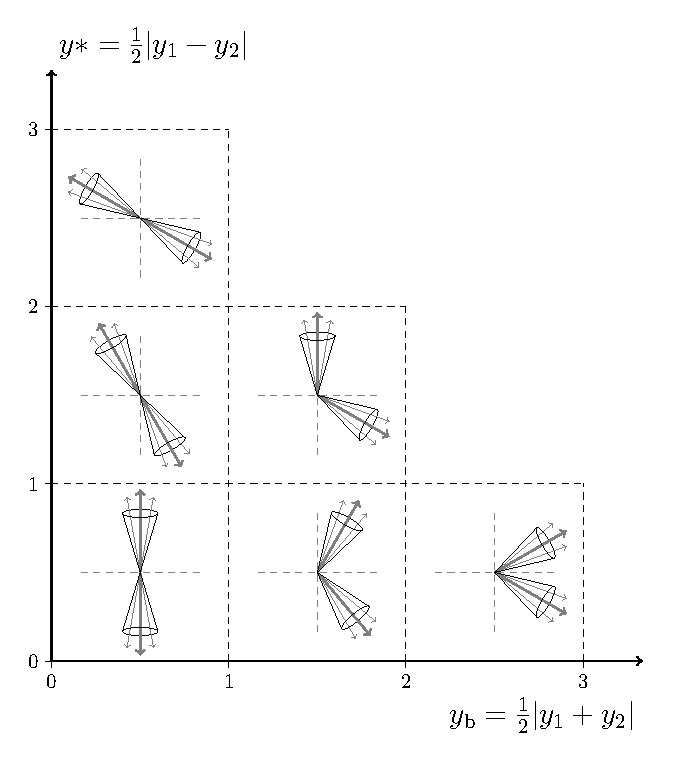
\includegraphics[width=0.9\textwidth]{figures/measurement/ybys.pdf}
    \caption{A descriptive representation of the dijet topologies in the various
    \ystar and \yboost bins. The binning separates in same side dijet
    events and opposite side dijet events which allows to draw conclusions about
    the initial state parton properties.}
    \label{fig:ysyb_schema}
\end{figure}

The differentiation in SS and OS dijet events is especially interesting since
both event topologies must access different fractional proton momenta while the
jets manifest themselves in the same (forward) detector region. Therefore
differences in the predictions can be attributed to the PDFs. This is clearly
visible in Fig.~\ref{fig:pdf_uncertainties} which shows the PDF uncertainties of
the cross section calculations. The measurement bin containing the events with
the large rapidity separation, see bottom right plot, has a significant larger
PDF uncertainty since there the high fractional proton momenta are accessed,
which are not well known.

\section{NLO Prediction}

The NLO cross section of the triple-differential dijet cross section is
calculated using fastNLO~\cite{Kluge:2006xs,Britzger:2012bs}. The fastNLO interpolation tables are
filled with the perturbative coefficients of the \NLOJETPP program~\cite{Nagy:2003tz}, see
Sec.~\ref{sec:nlojetpp}. The PDFs are accessed via the LHAPDF
library~\cite{lhapdf}. The \as-evolution is done using the provided routines
by the PDF sets. The advantage of the application of the fastNLO framework
instead of direct calculation using \NLOJETPP is the possibility to repeat the
calculations using different PDFs and scale choices as it is neccessary to
calculate the PDF and scale uncertainties.

\subsection{Scale Choice}

Within the perturbative cross section calculations, one has to choose a
factorization and renormalization scale. The influence of these scales vanishes
when the calculation is performed for all orders of the perturbative series.
However since we truncate the series at NLO, a scale dependence on our result is
introduced. Three possibilities of the scale choice are studied in this thesis.
The most natural scale choice which reflects the energy scale of the measurement
is to use the average \pt of the dijet system as the renormalization and
factorization scale as it is also used as the binning variable. 

\begin{equation*}
    \mu = \mur = \muf = \frac{p_{\mathrm{T},1} + p_{\mathrm{T},2}}{2}
\end{equation*}

While this scale choice yields reasonable results, the $k$-factor and scale
uncertainties indicate problems, which are discussed in detail
in the next sections. The second investigated scale choice is based on the
findings of a recent study by ATLAS~\cite{Aad:2011fc}. They claim that
fixed-order calculations which are binned in \ystar get unreliable for hig
\ystar values if the scale is only based on the energy. Based on recommendations
by theorists~\cite{Ellis:1992en}, a scale which also introduces a dependence on
the rapdity separation is proposed.

\begin{equation*}
    \mu = \mur = \muf = p_{\mathrm{T,max}} e^{0.3 \ystar} 
\end{equation*}

Additionally a variation oft this choice was studied in which the scale is not
dependent on the transverse momentum of the leading jet but on the average
transverse momentum of the leading two jets.

\begin{equation*}
    \mu = \mur = \muf = p_{\mathrm{T,avg}} e^{0.3 \ystar} 
\end{equation*}

Fig.~\ref{fig:xs_nlo_comp} shows the prediction of the NLO calculation using
the three mentioned scale choices. The cross section predicted by each of
calculations is similar with larger deviations for the scale choice using the
maximum transverse momentum instead of the average dijet transverse momentum.
The differences between the predictions are covered by the scale uncertainties
afflicted to the prediction.


\begin{figure}[htp]
    \centering
    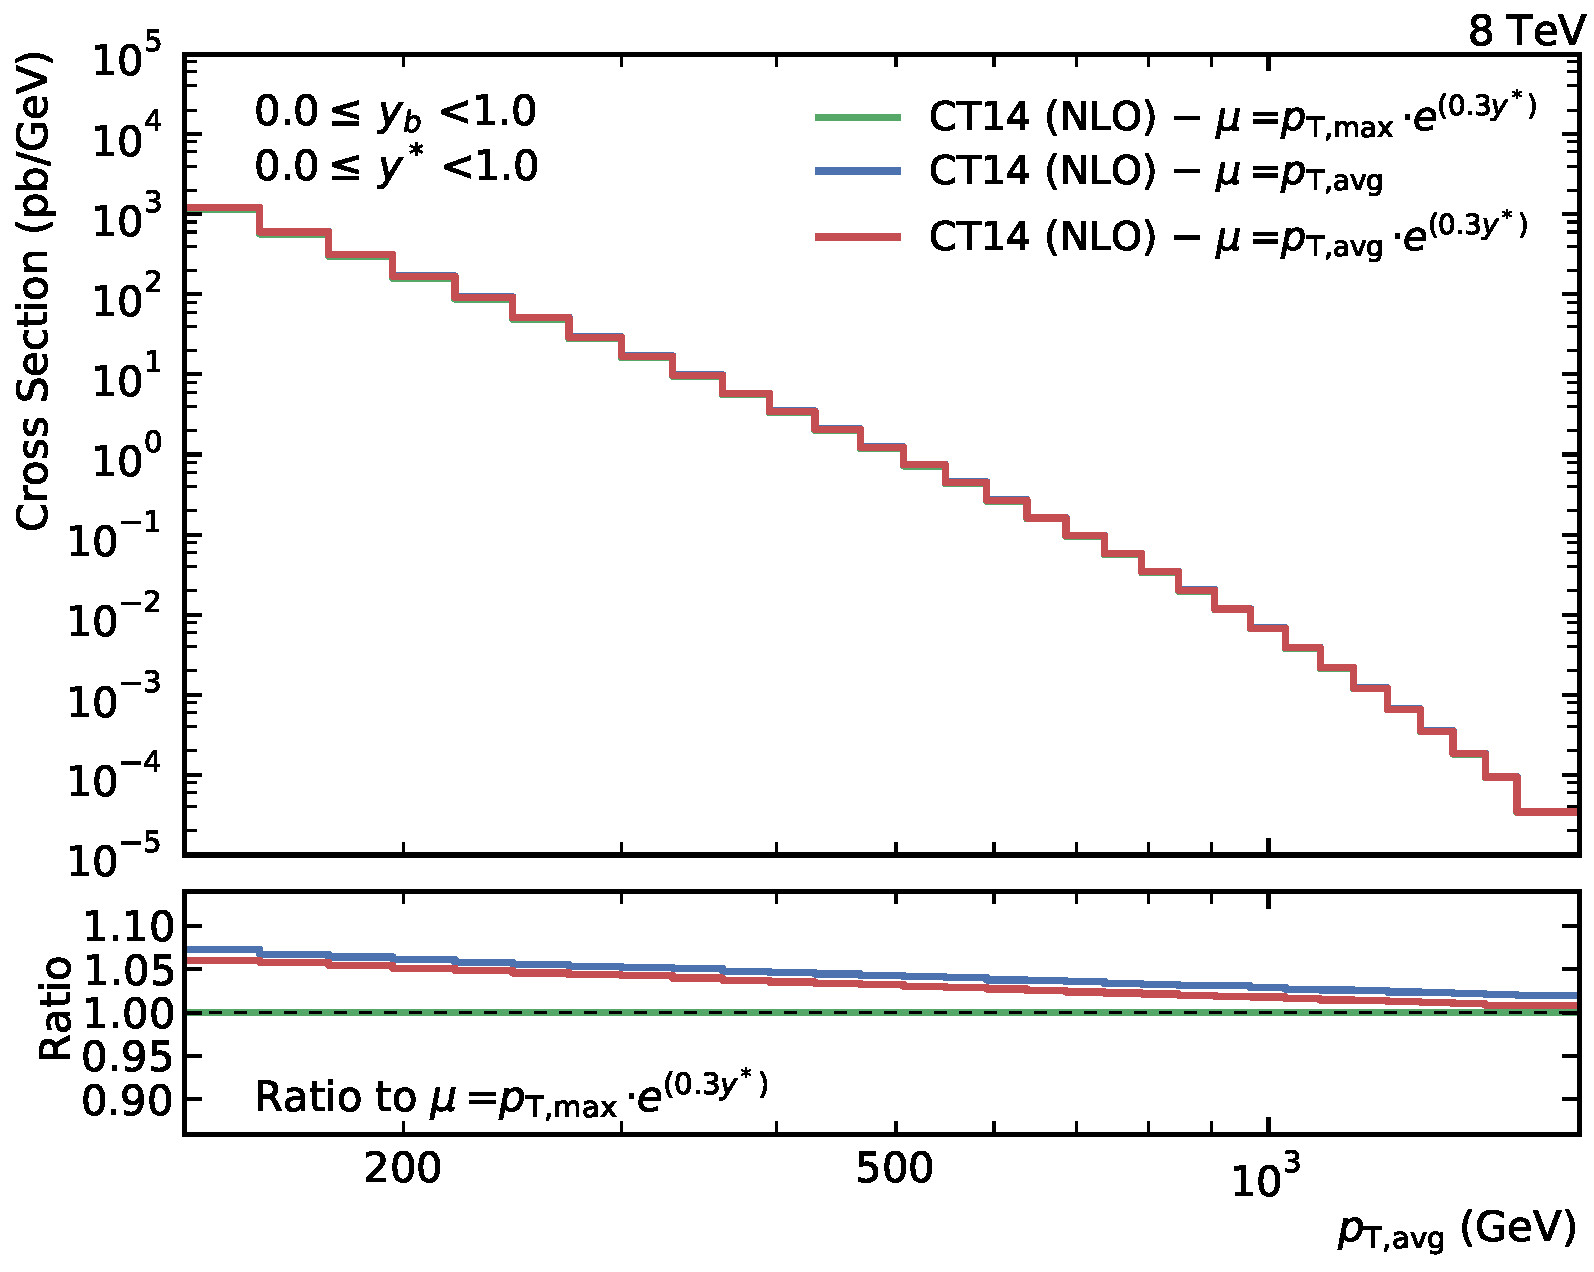
\includegraphics[width=0.45\textwidth]{figures/theory/nlo_xs_comp_yb0ys0.pdf}\hfill
    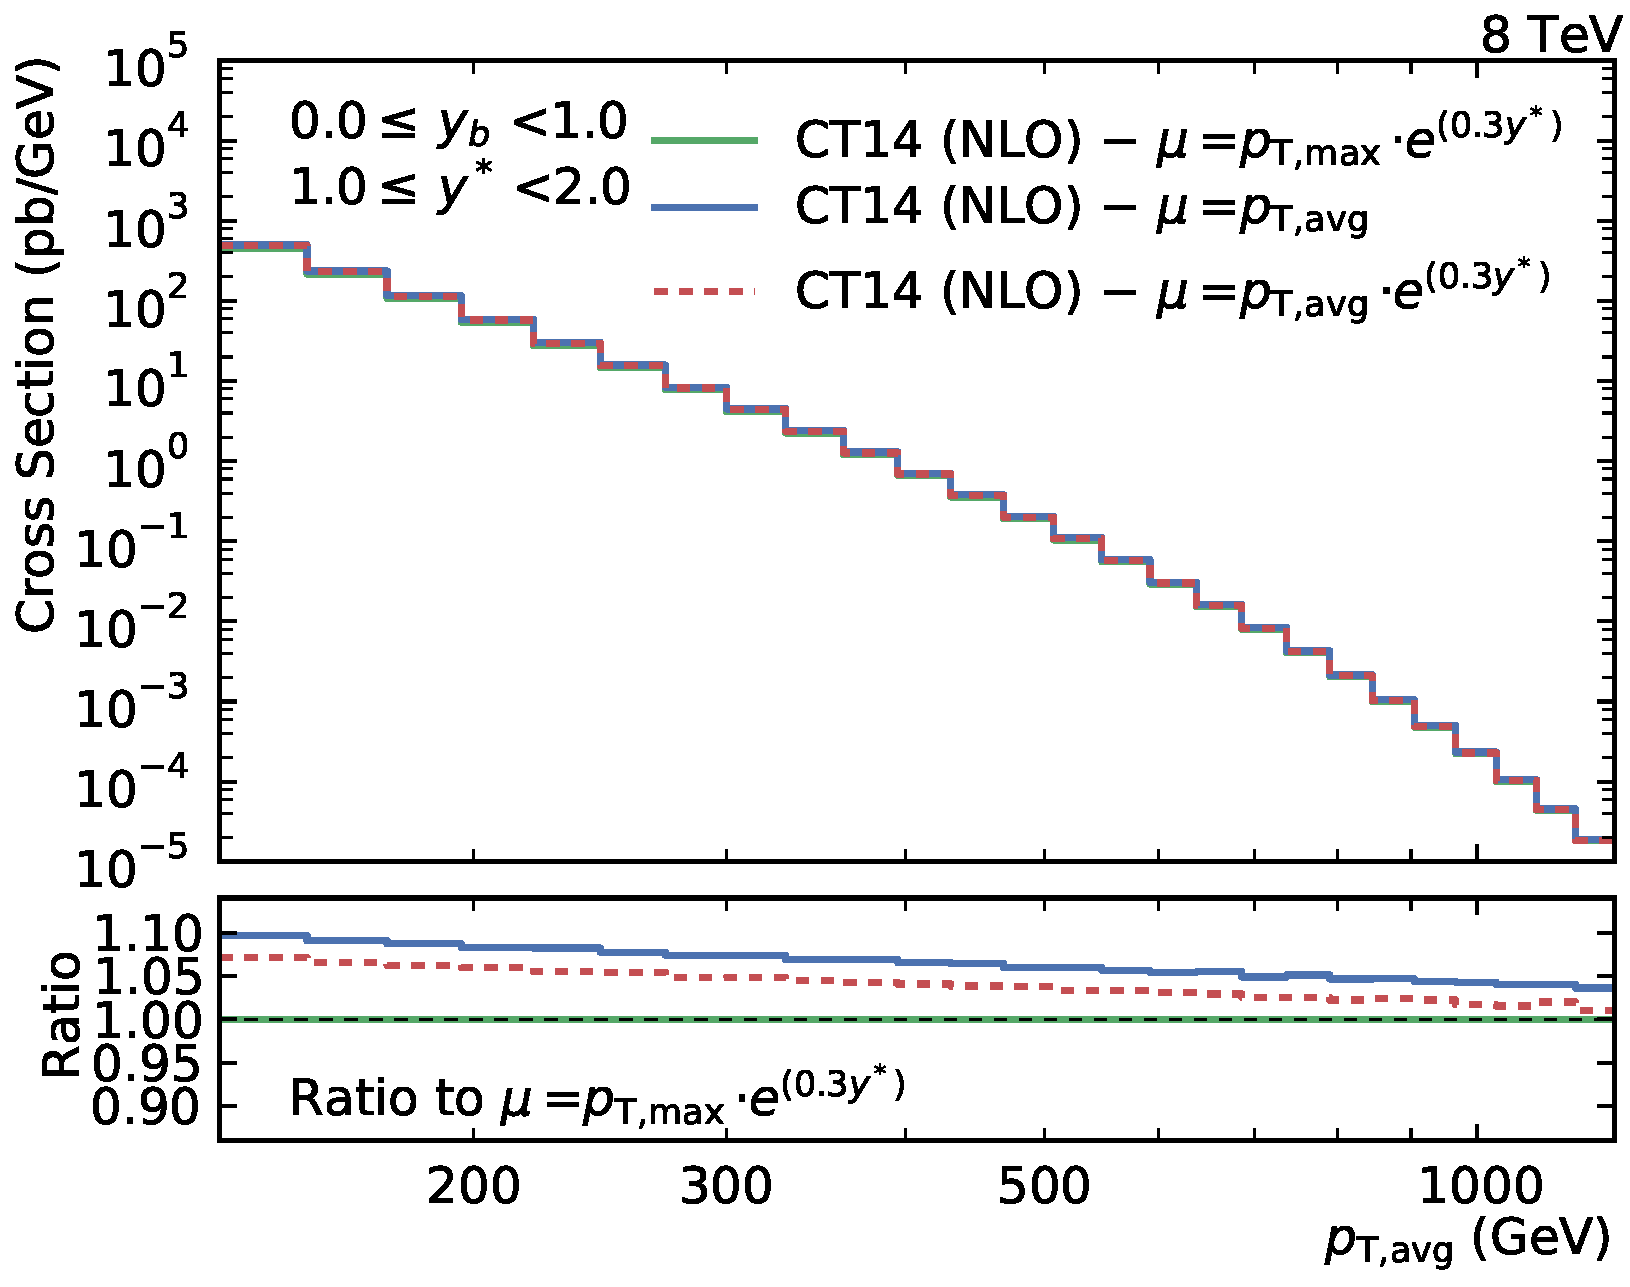
\includegraphics[width=0.45\textwidth]{figures/theory/nlo_xs_comp_yb0ys1.pdf}
    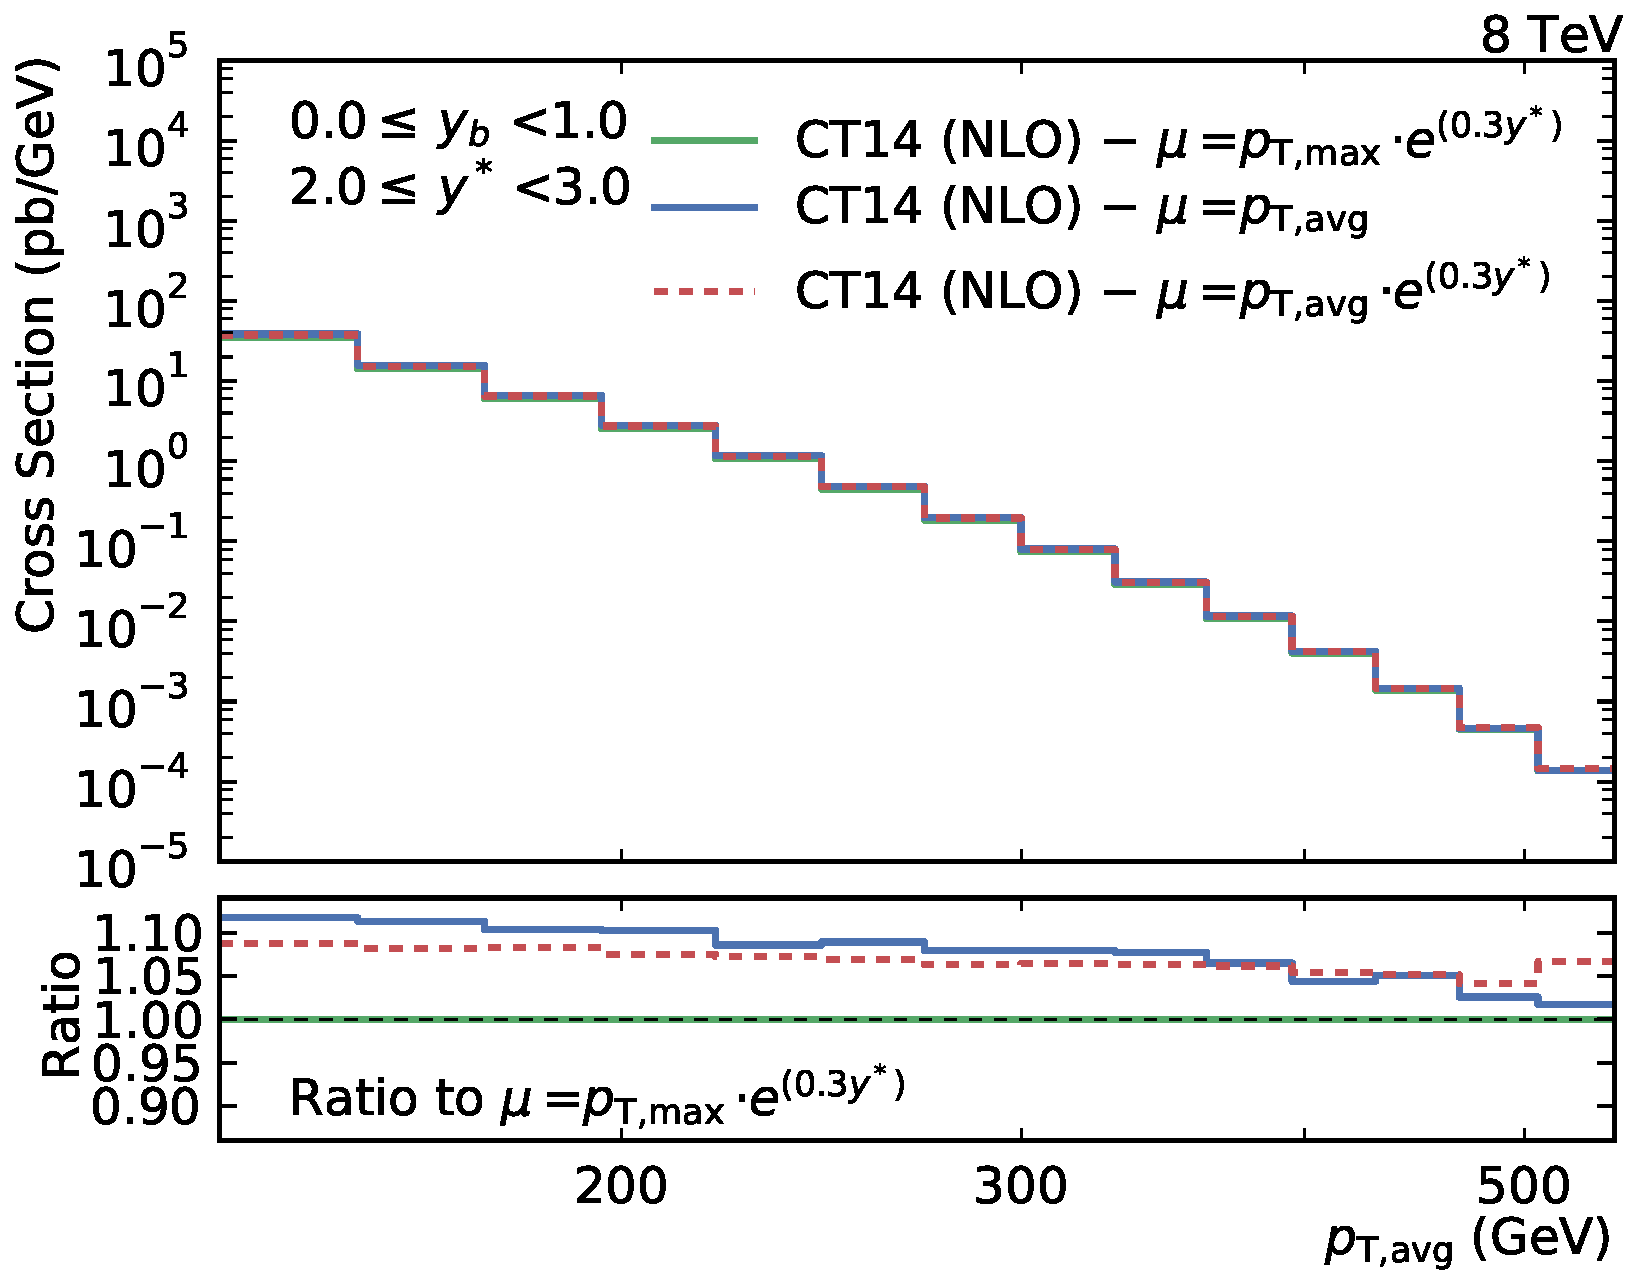
\includegraphics[width=0.45\textwidth]{figures/theory/nlo_xs_comp_yb0ys2.pdf}\hfill
    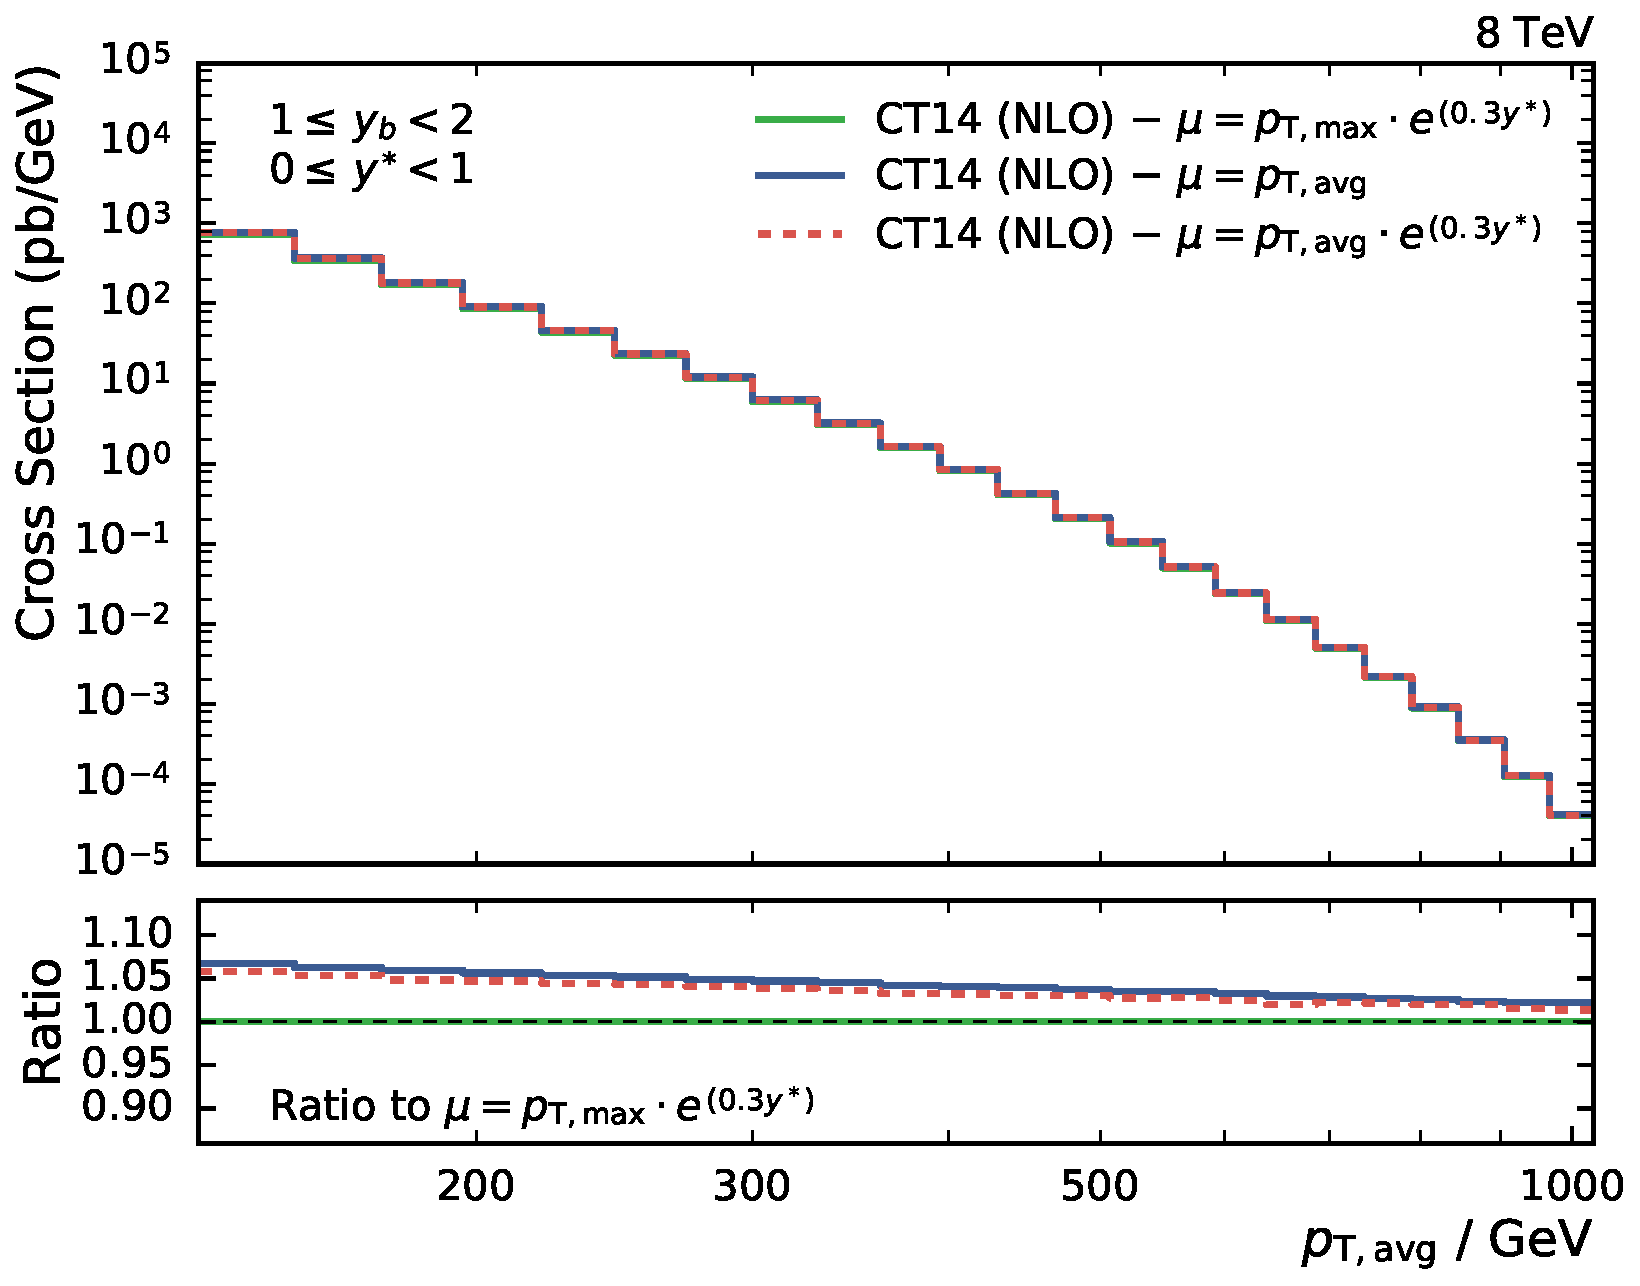
\includegraphics[width=0.45\textwidth]{figures/theory/nlo_xs_comp_yb1ys0.pdf}
    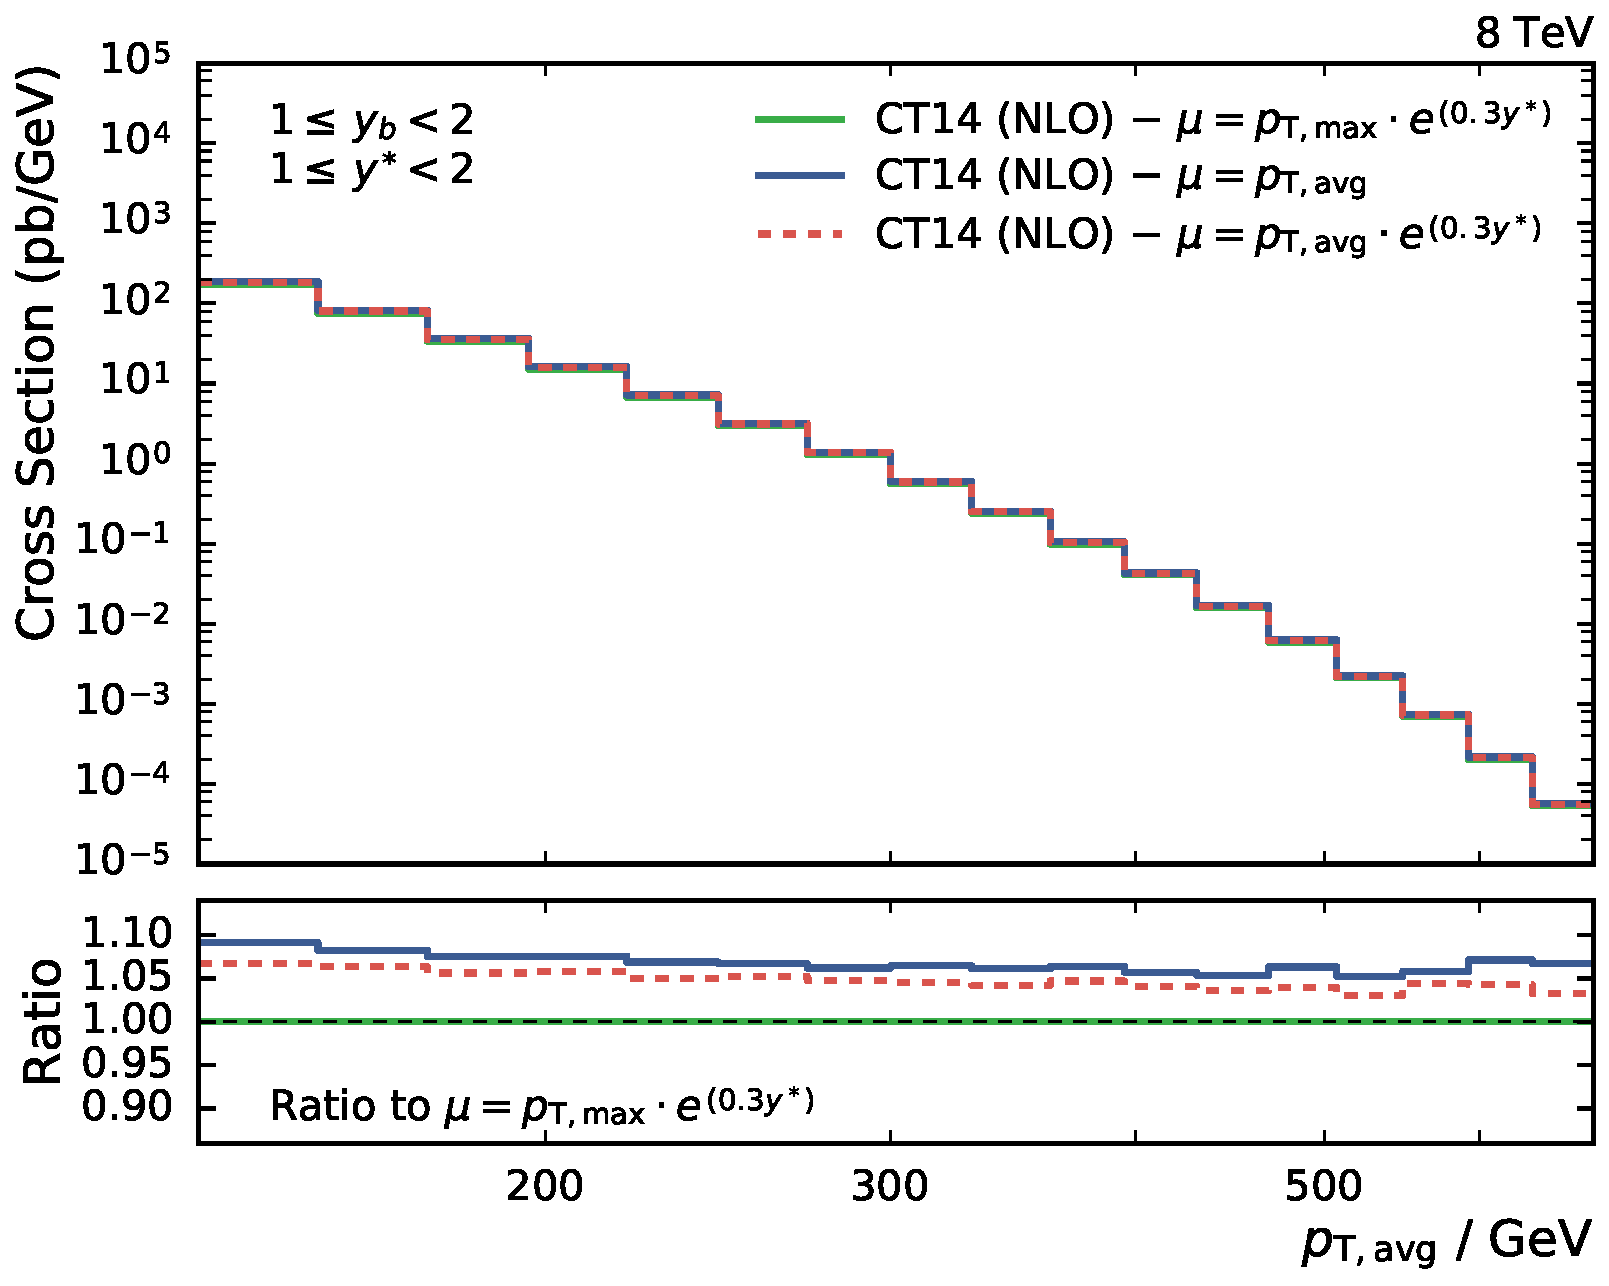
\includegraphics[width=0.45\textwidth]{figures/theory/nlo_xs_comp_yb1ys1.pdf}\hfill
    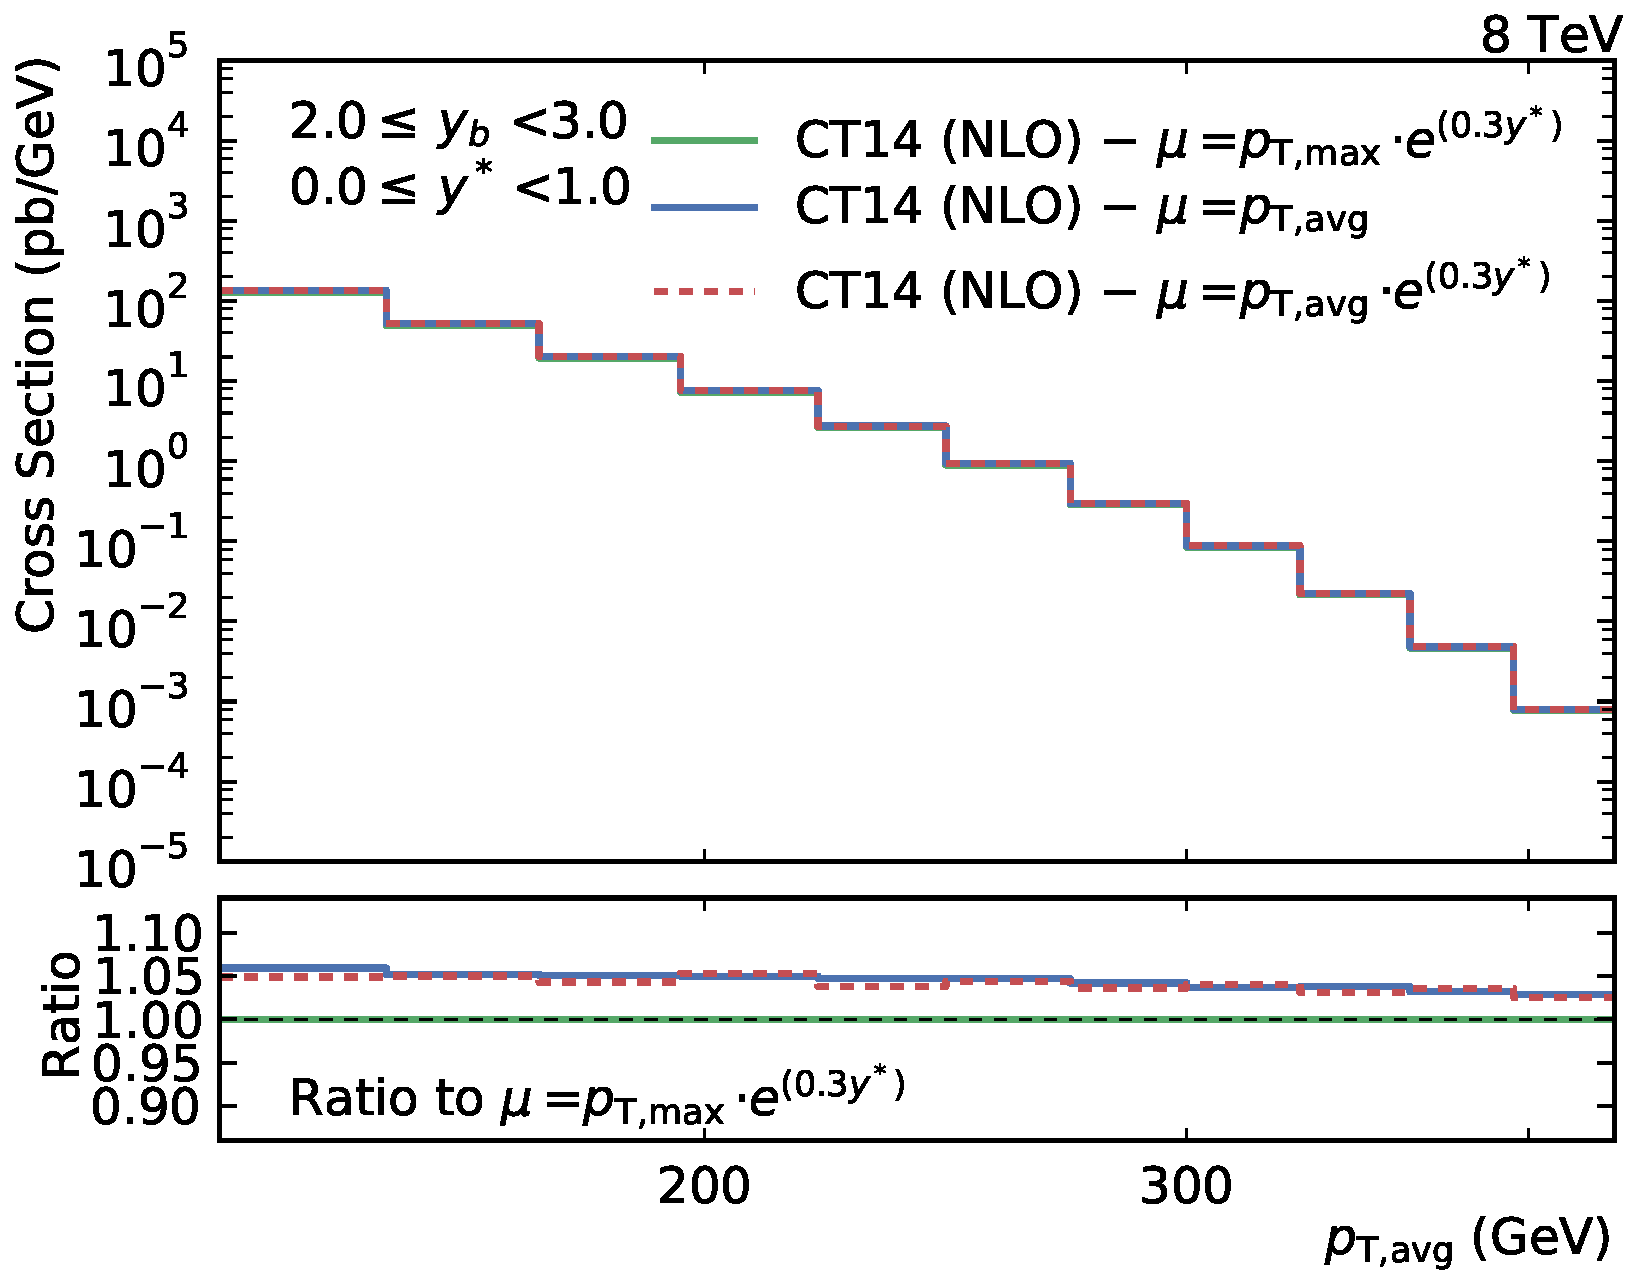
\includegraphics[width=0.45\textwidth]{figures/theory/nlo_xs_comp_yb2ys0.pdf}
    \caption{The NLO prediction \NLOJETPP for the dijet measurement. The
    predictions of three different scale choices are shown. In almost all cases
    the differences between the calculations are covered by the scale uncertainties.}
    \label{fig:xs_nlo_comp}
\end{figure}


\subsection{NLO $k$-factors}

To check the influence of the higher-order contributions to the perturbative QCD
prediction, one calculates the differences between the LO prediction and the NLO
prediction, expressed as the ratio $k_\mathrm{NLO}$.

\begin{equation*}
    k_{\mathrm{NLO}} = \frac{\sigma_{\mathrm{NLO}}}{\sigma_{\mathrm{LO}}}
\end{equation*}

The size of the NLO correction gives an estimation about the influence of these
higher-order corrections. If they are very small, the LO result already
describes the observable cross section precisely. It is also possible that the
$k$-factors fall below unity, in which the NLO corrections are negative and the
total cross section decreases when adding the correction.
Fig.~\ref{fig:kfactor_comp} shows the $k$-factors of obtained by the prediction
using the different scale choices. The $k$-factors are similar in the central
region, but get quite different in regions with larger rapidity separations.
Especially the $k$-factors in the \ystar bin from 2.0 to 3.0 shows a $k$-factor
smaller one for the \ptavg scale choice while it is larger than one for the
scale choices including the \ystar dependence.


\begin{figure}[htp]
    \centering
    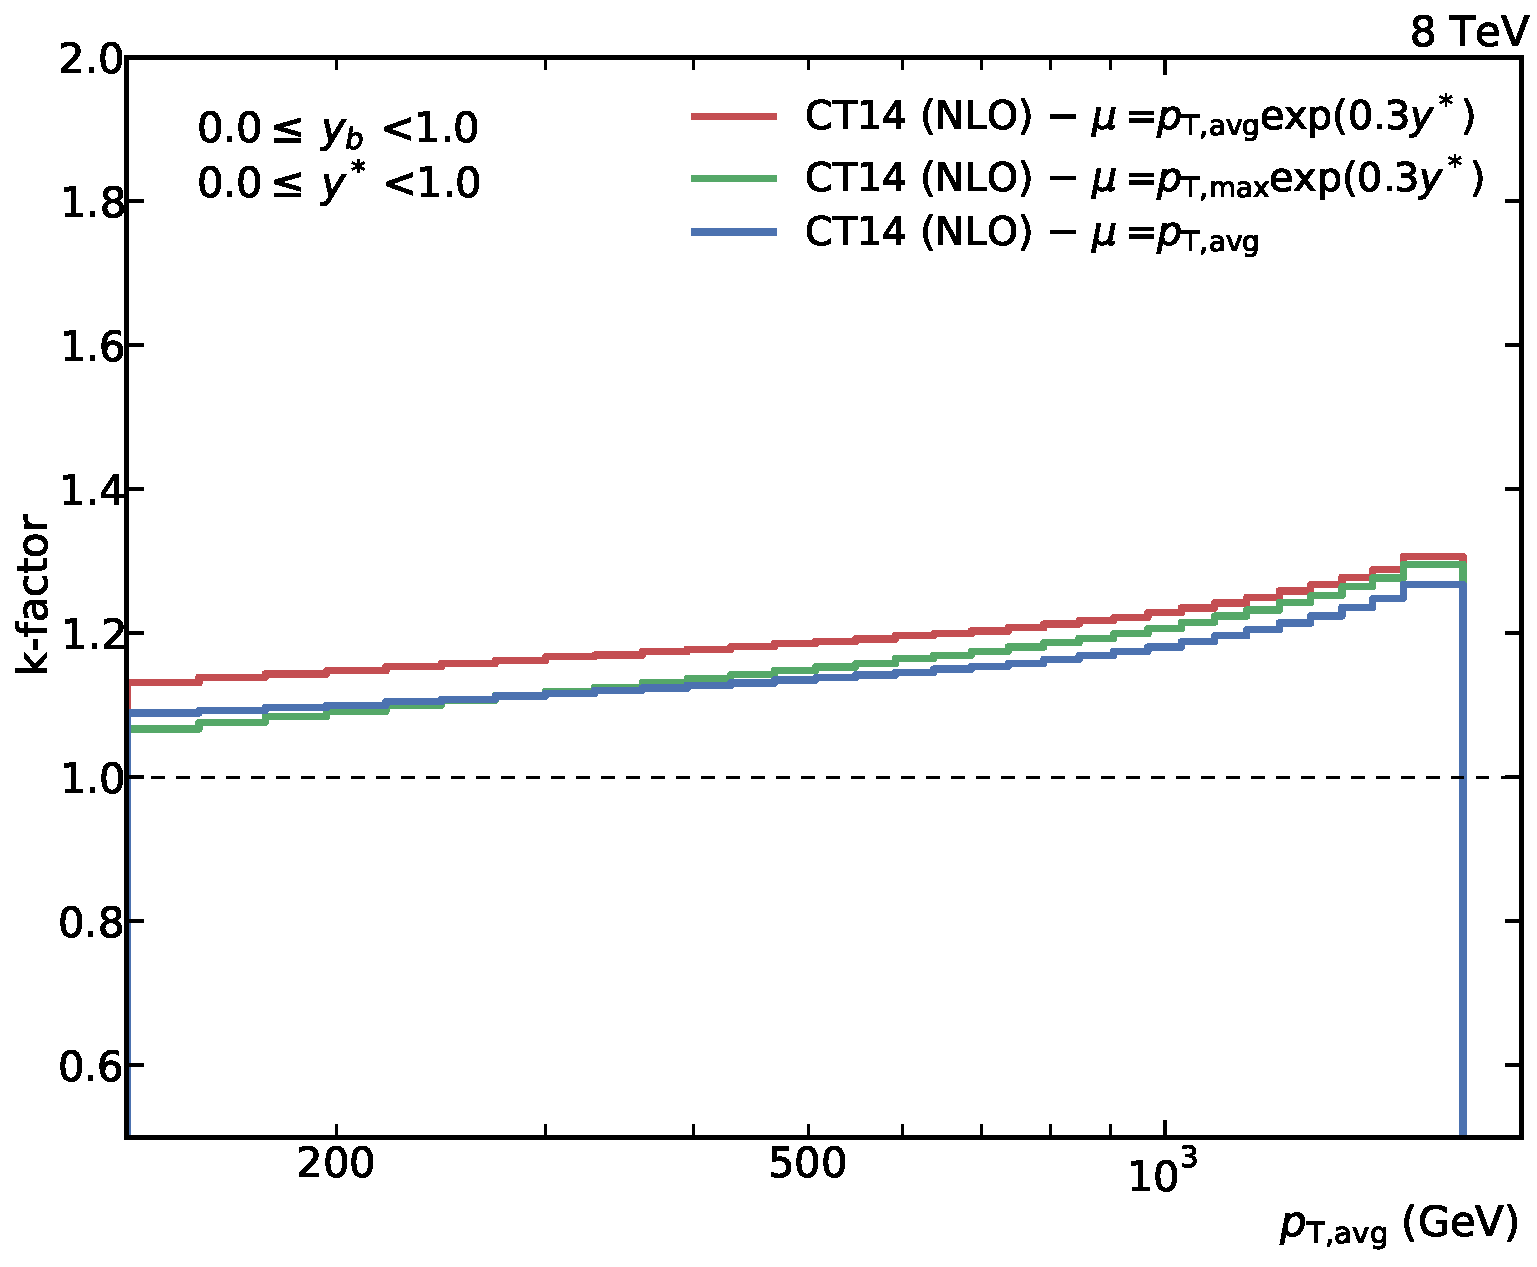
\includegraphics[width=0.45\textwidth]{figures/theory/kfactor_comp_yb0ys0.pdf}\hfill
    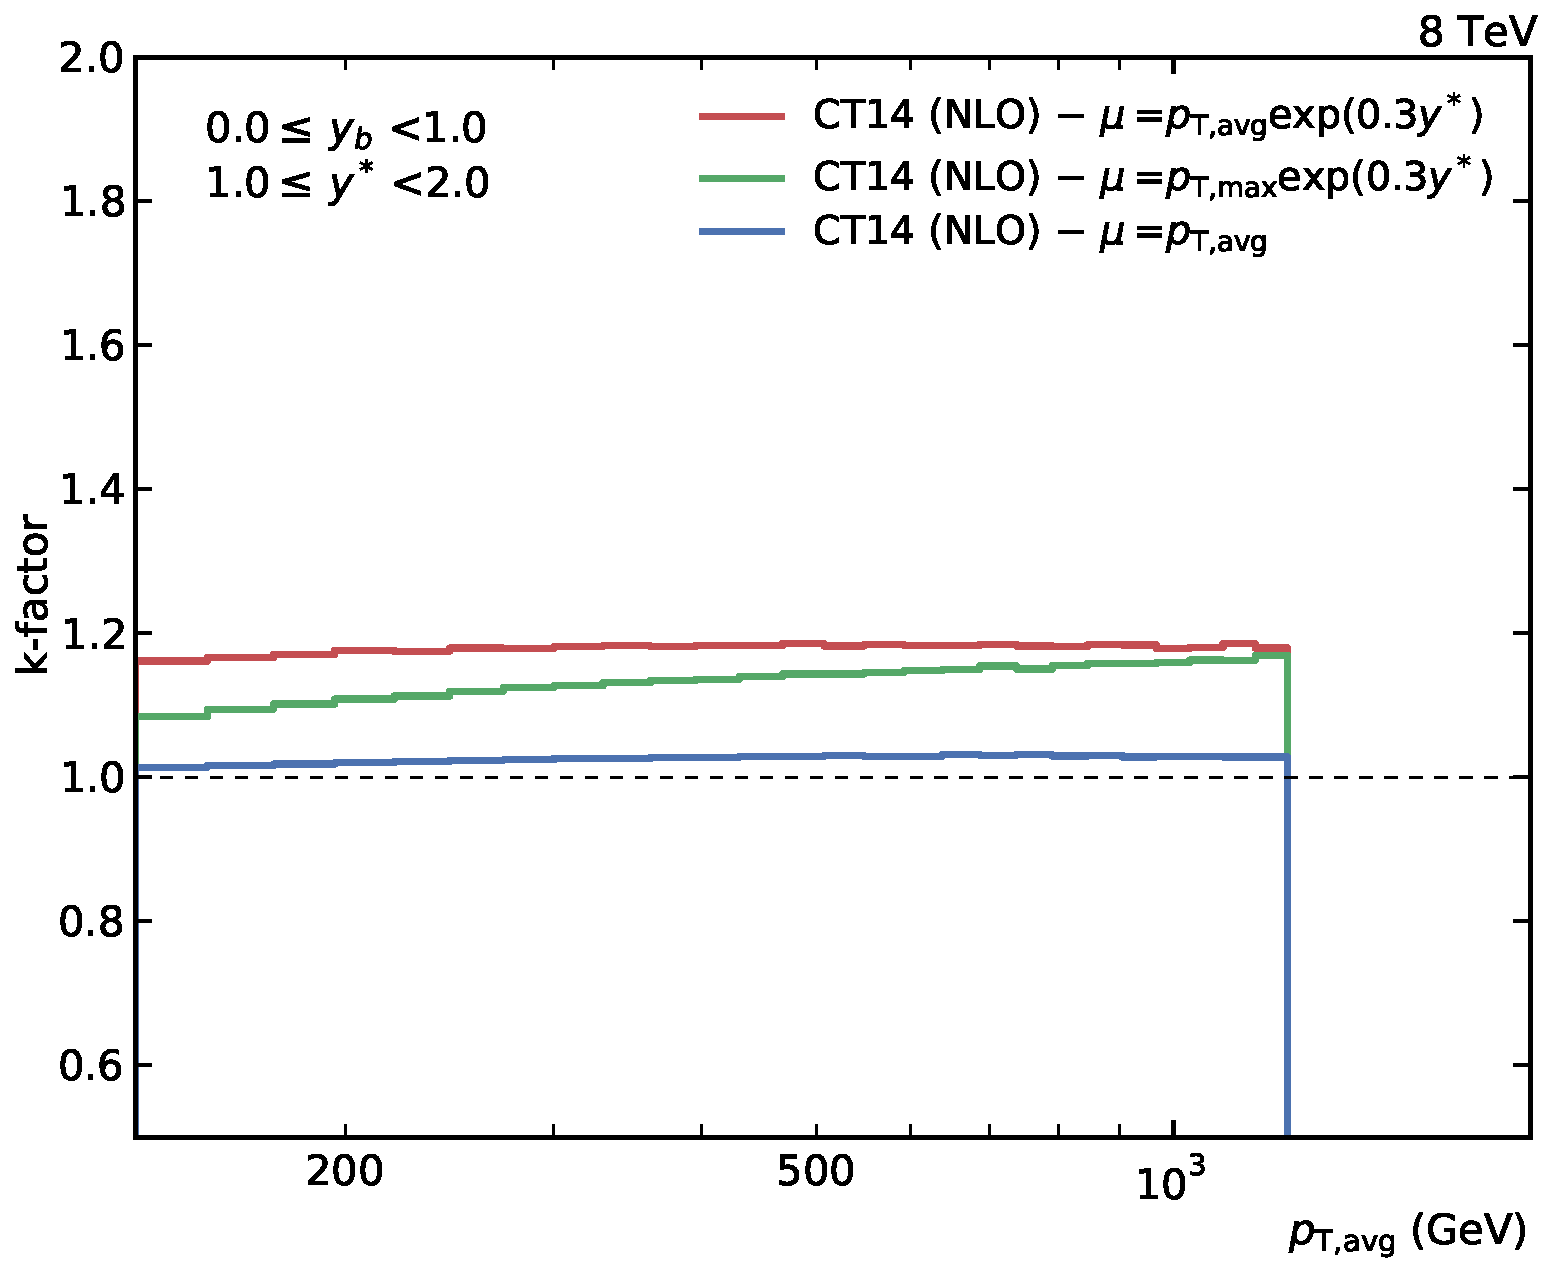
\includegraphics[width=0.45\textwidth]{figures/theory/kfactor_comp_yb0ys1.pdf}
    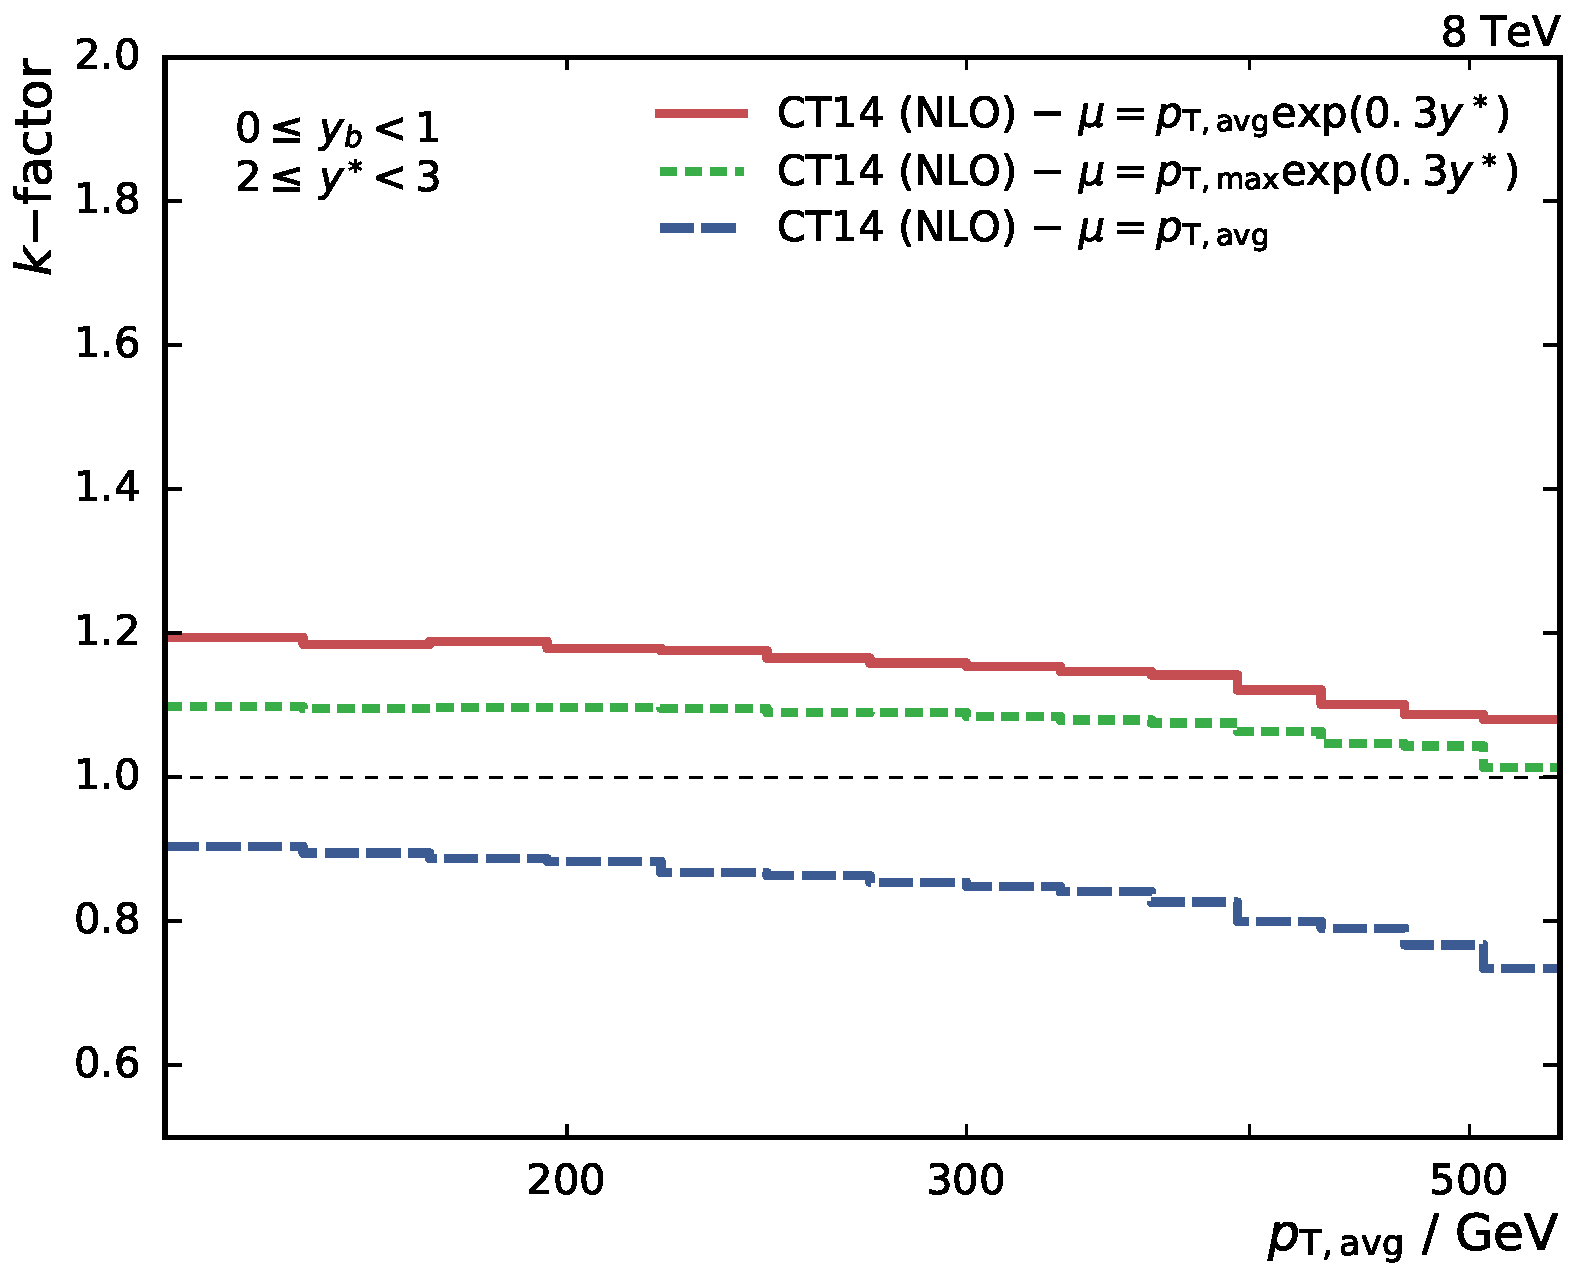
\includegraphics[width=0.45\textwidth]{figures/theory/kfactor_comp_yb0ys2.pdf}\hfill
    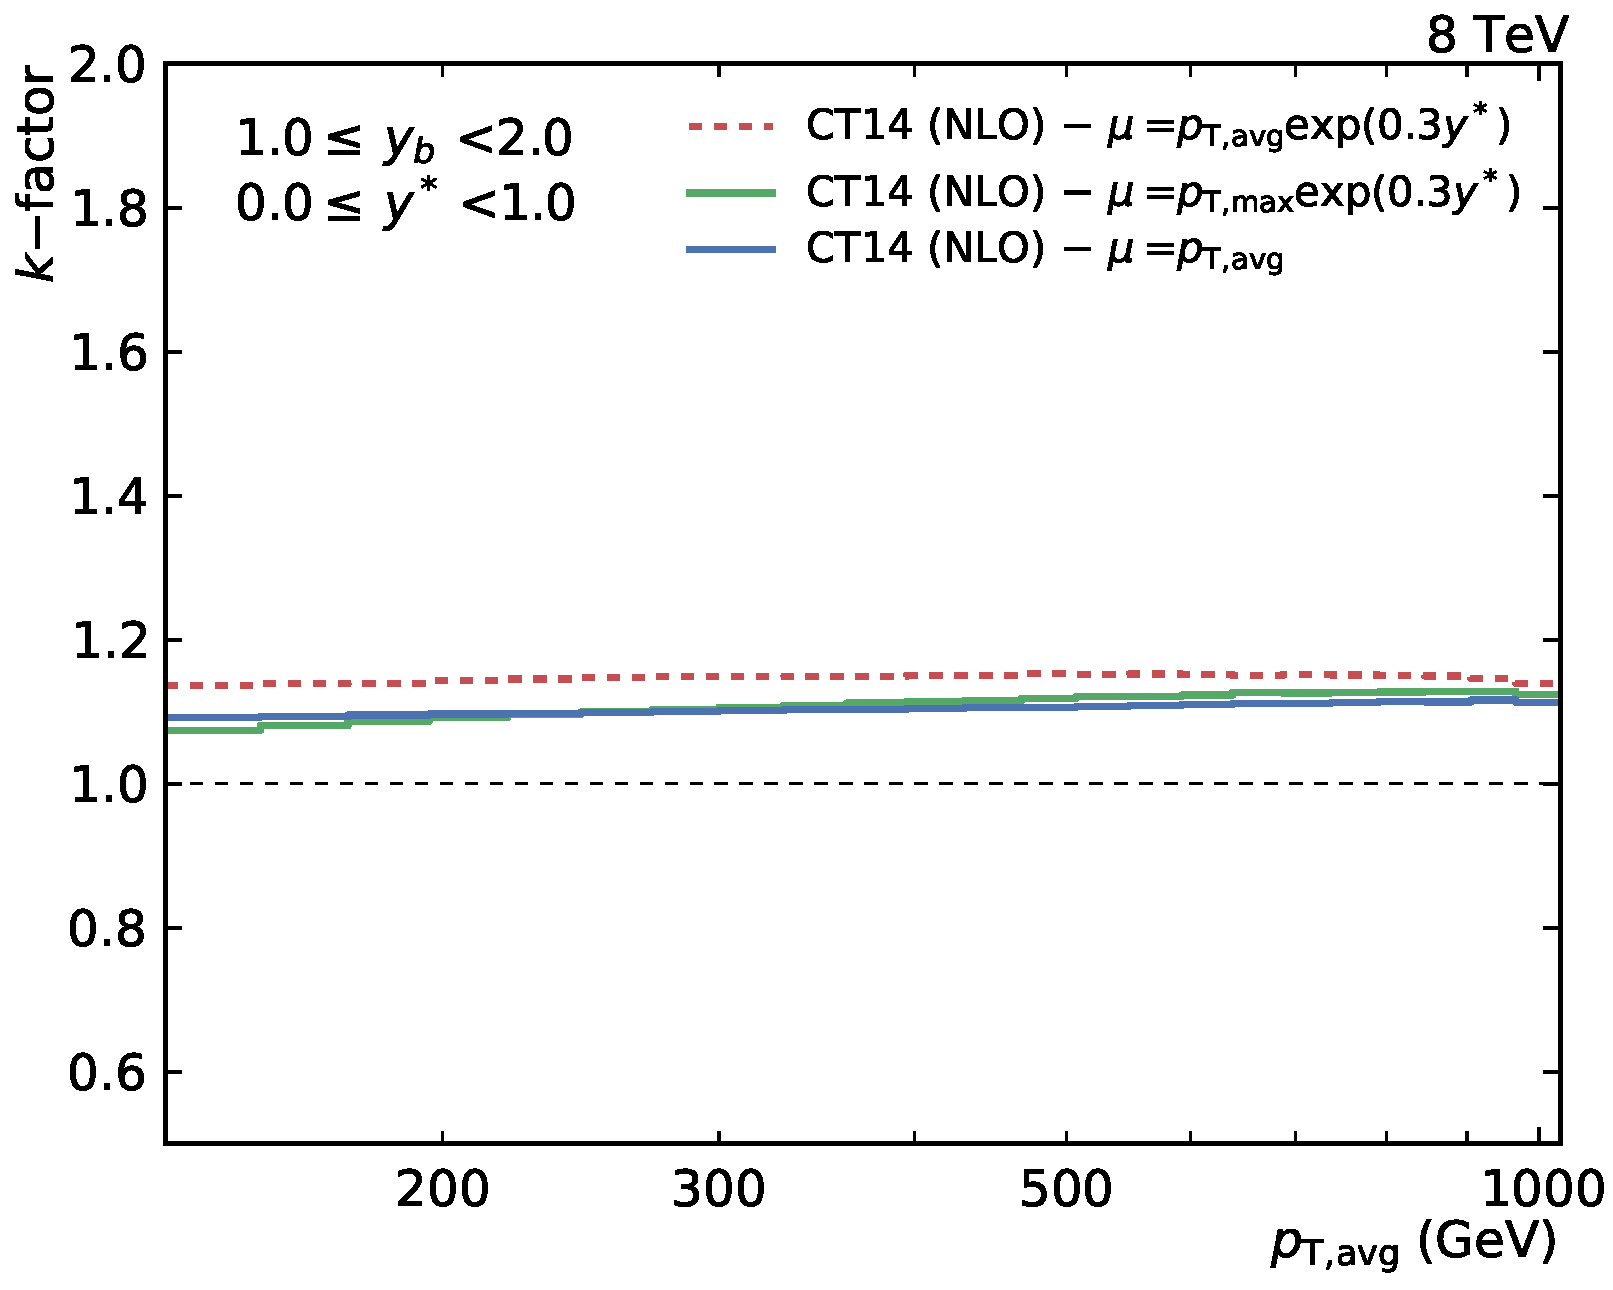
\includegraphics[width=0.45\textwidth]{figures/theory/kfactor_comp_yb1ys0.pdf}
    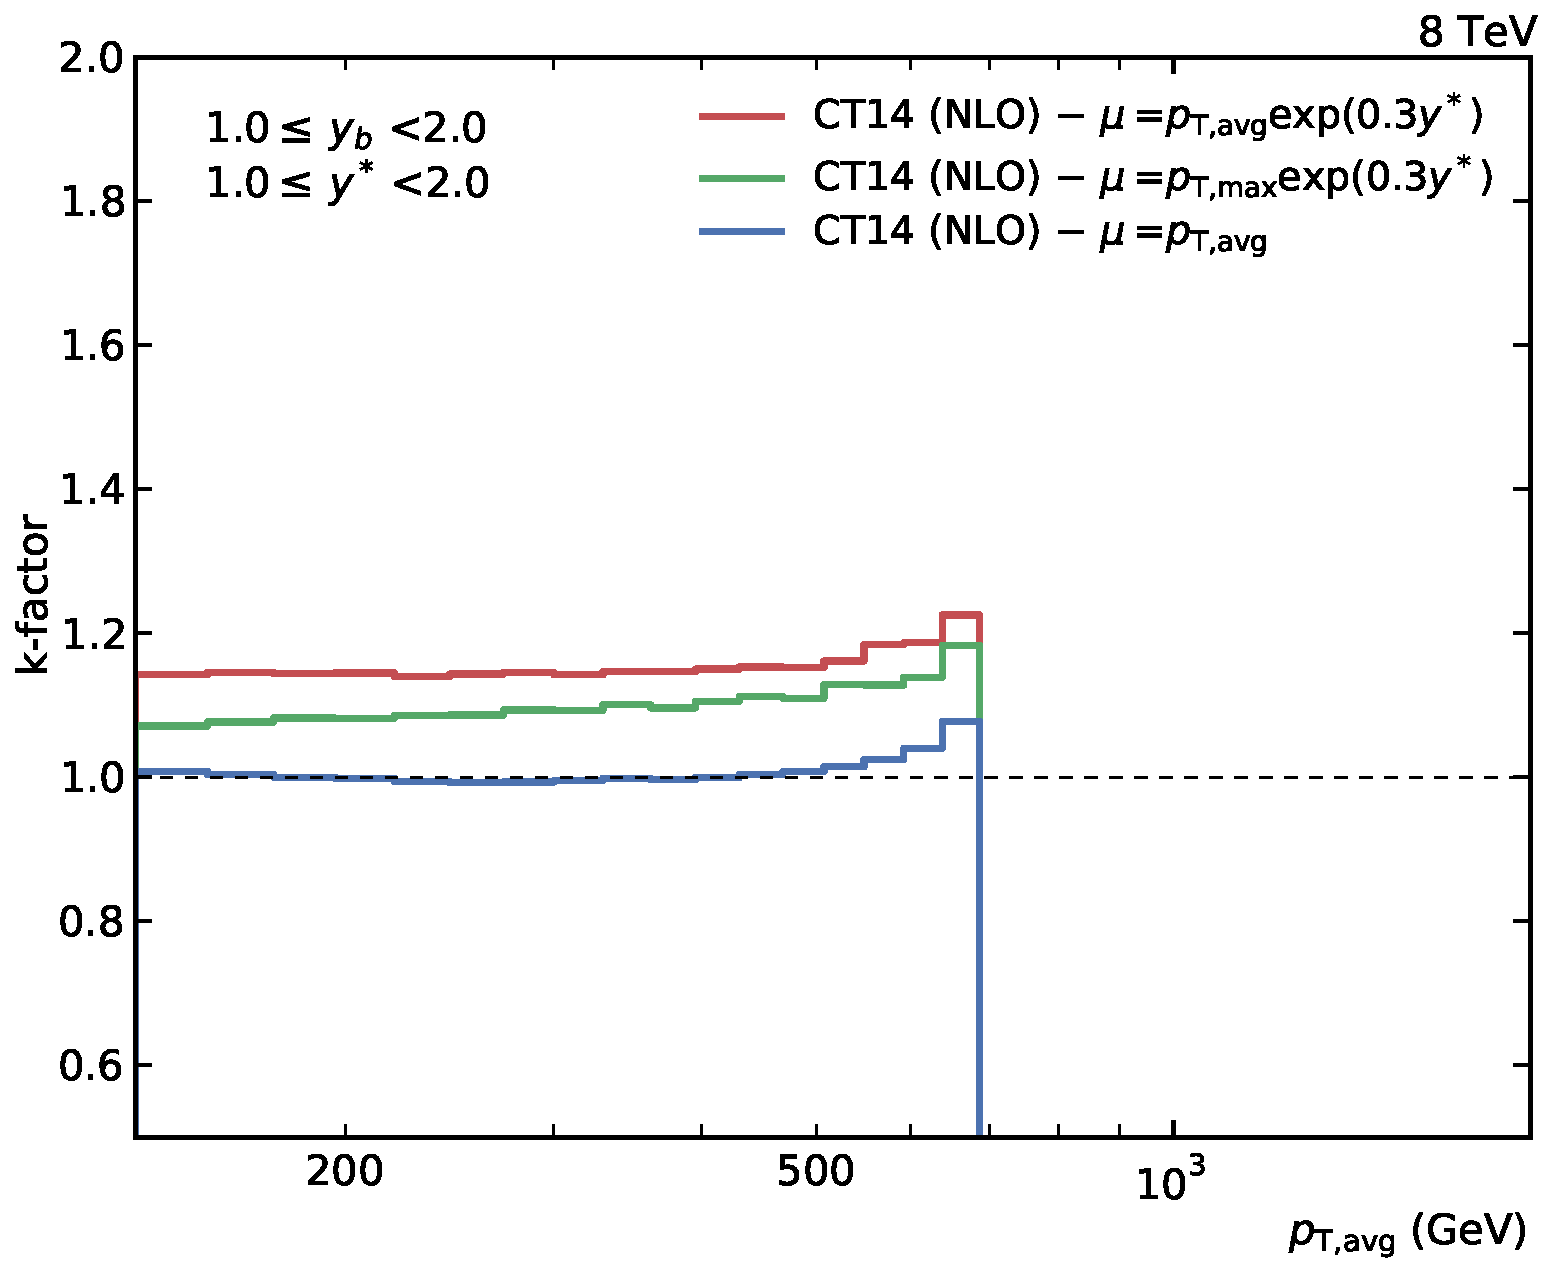
\includegraphics[width=0.45\textwidth]{figures/theory/kfactor_comp_yb1ys1.pdf}\hfill
    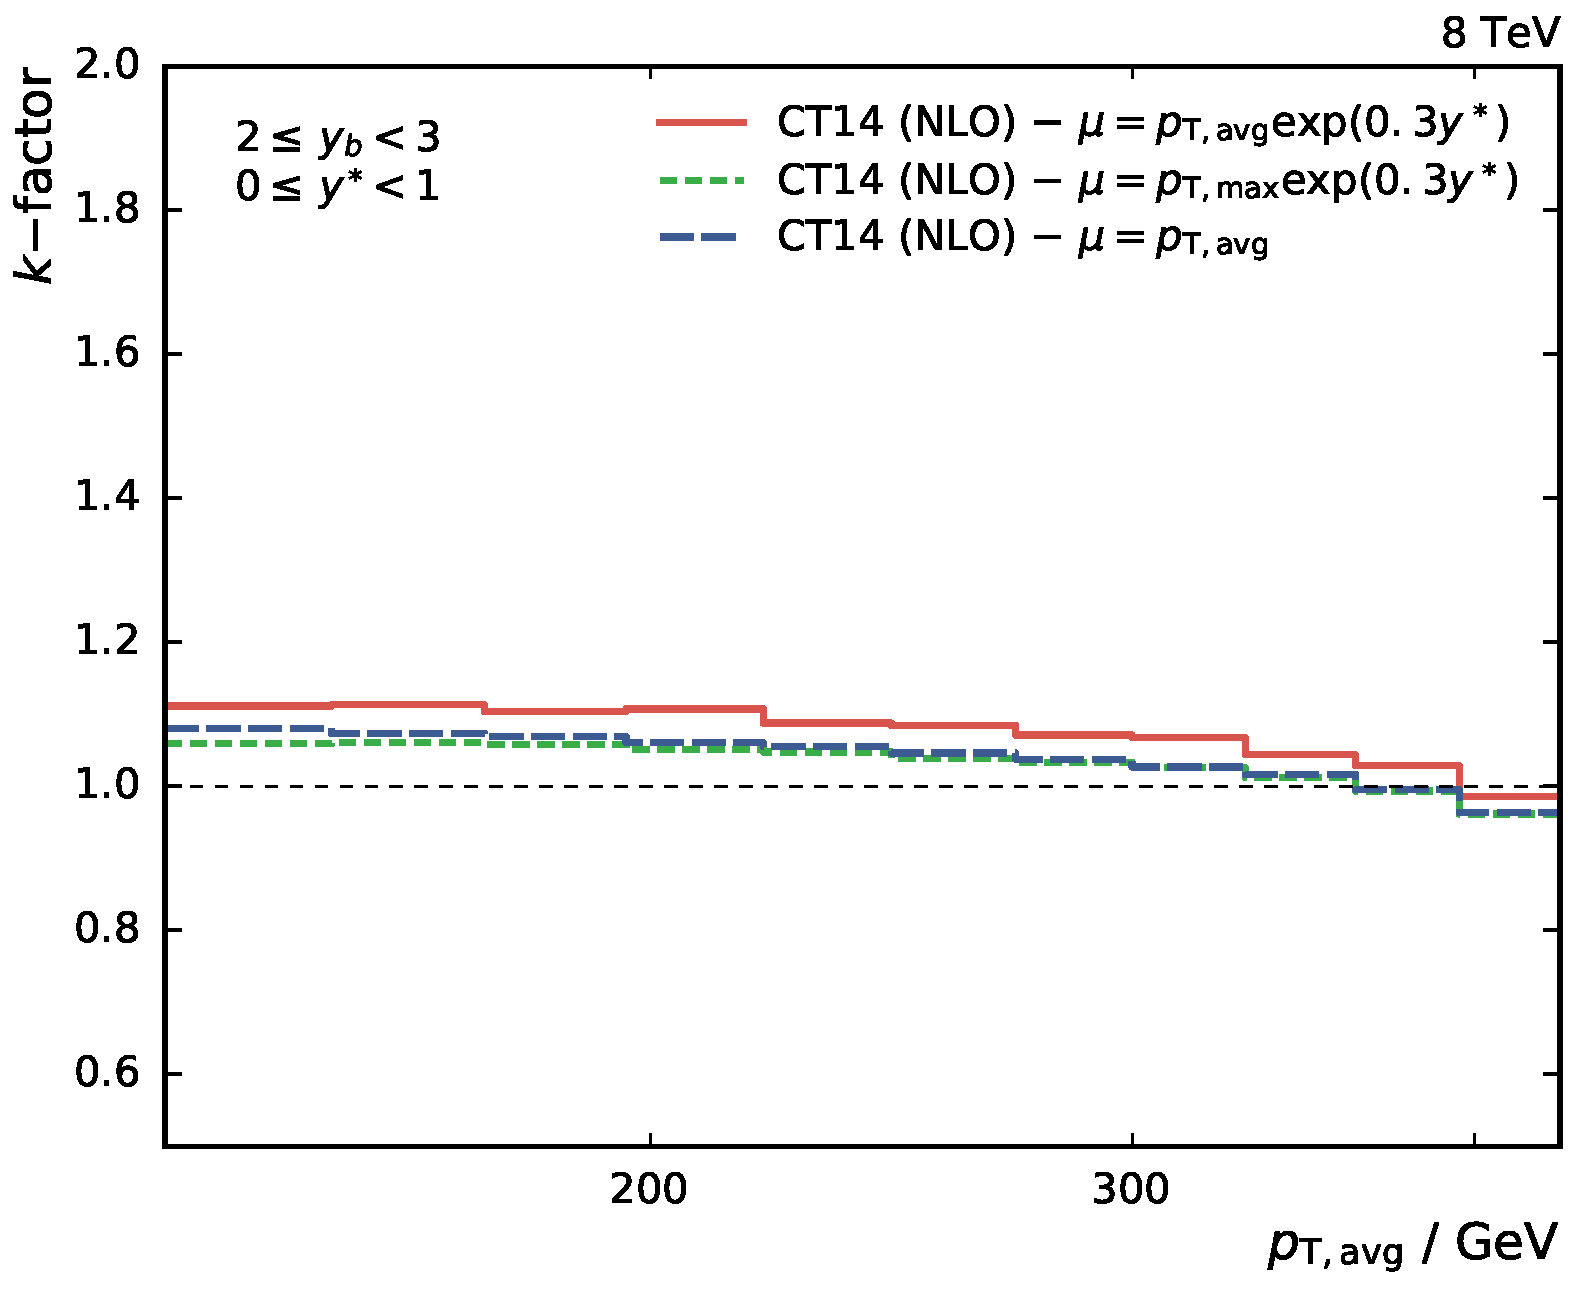
\includegraphics[width=0.45\textwidth]{figures/theory/kfactor_comp_yb2ys0.pdf}
    \caption{The $k$-factor between the LO calculation and the NLO calculation
    shows the influence of the higher-order correction terms. The $k$-factors
for the calculation with \ptavg as scale choice fall below unity in case of high
\ystar values indicating that the NLO correction is negative.}
    \label{fig:kfactor_comp}
\end{figure}


\section{Non-Perturbative Corrections}

\NLOJETPP gives a NLO cross section at parton level. These fixed-order
perturbative calculations do not consider effects from hadronization or multiple
parton interaction (MPI) as they can not be described in a perturbative
calculation. To be able to
compare fixed-order cross sections with the unfolded measurement, which yields a
cross section at particle level, so-called non-perturbative (NP) corrections are
calculated and applied to the parton level prediction. These corrections must be
calculated using a MC event generator which is able to simulate MPI and
hadronization. The correction is obtained by calculating the ratio between the
nominal cross section using all simulation steps and a cross section calculation
without hadronization and MPI enabled, see Eq.~\ref{eq:np_definition}. The
correction is then applied as a bin-by-bin correction factor to the NLO cross
section.

\begin{equation}
    C^{\mathrm{NP}} = \frac{N^{\mathrm{PS+HAD+MPI}}}{N^{\mathrm{PS}}}
    \label{eq:np_definition}
\end{equation}

The non-perturbative corrections have been calculated using two Monte Carlo
event generators using the newest available tune within CMS. Herwig++ is used
with the tune UE-EE-5C and Pythia 8 with the tune CUETP8M1. The ratio is fitted
using a power-law function, see Eq.~\ref{fcn:np_fit}.

\begin{equation}
  f(\ptavg) = a \cdot \ptavg^b + c
  \label{fcn:np_fit}
\end{equation}

Since the correction factors obtained from Herwig++ and Pythia8 are quite
different in the low-\pt region, an uncertainty was assigned to the correction
factor. The average of both corrections is used as the final correction factors
and the envelope of the Pythia8 and the Herwig++ predictions are used as the
uncertainty.

Fig.~\ref{fig:np_factors} shows the resulting correction factors and the
corresponding uncertainty.  The corrections are of the size of 10 \% to 15 \% at
100 \si{GeV} and get smaller at higher values of \ptavg. While the correction
decreases for higher transverse momenta, it does not approach unity especially
in the bins containing jets with high rapidities. 

\begin{figure}[htp]
    \centering
    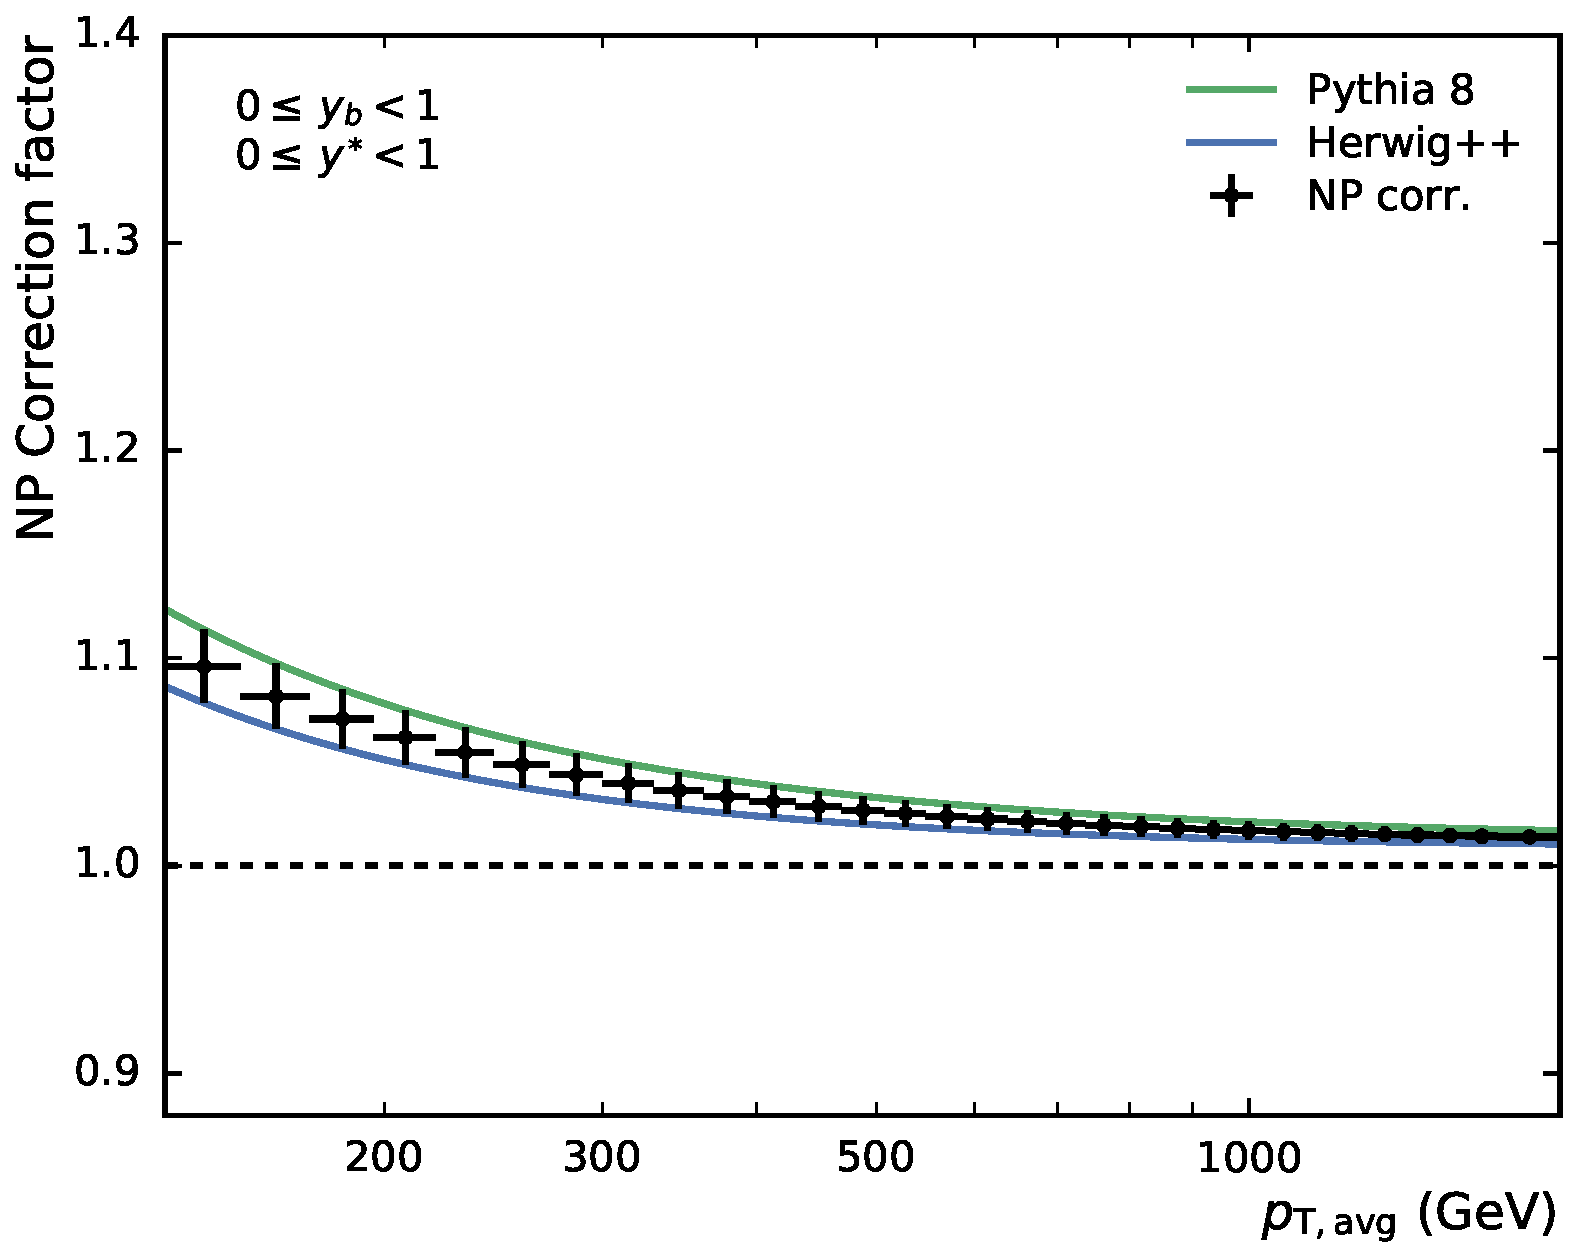
\includegraphics[width=0.45\textwidth]{figures/theory/np_factors_calc_yb0ys0.pdf}\hfill
    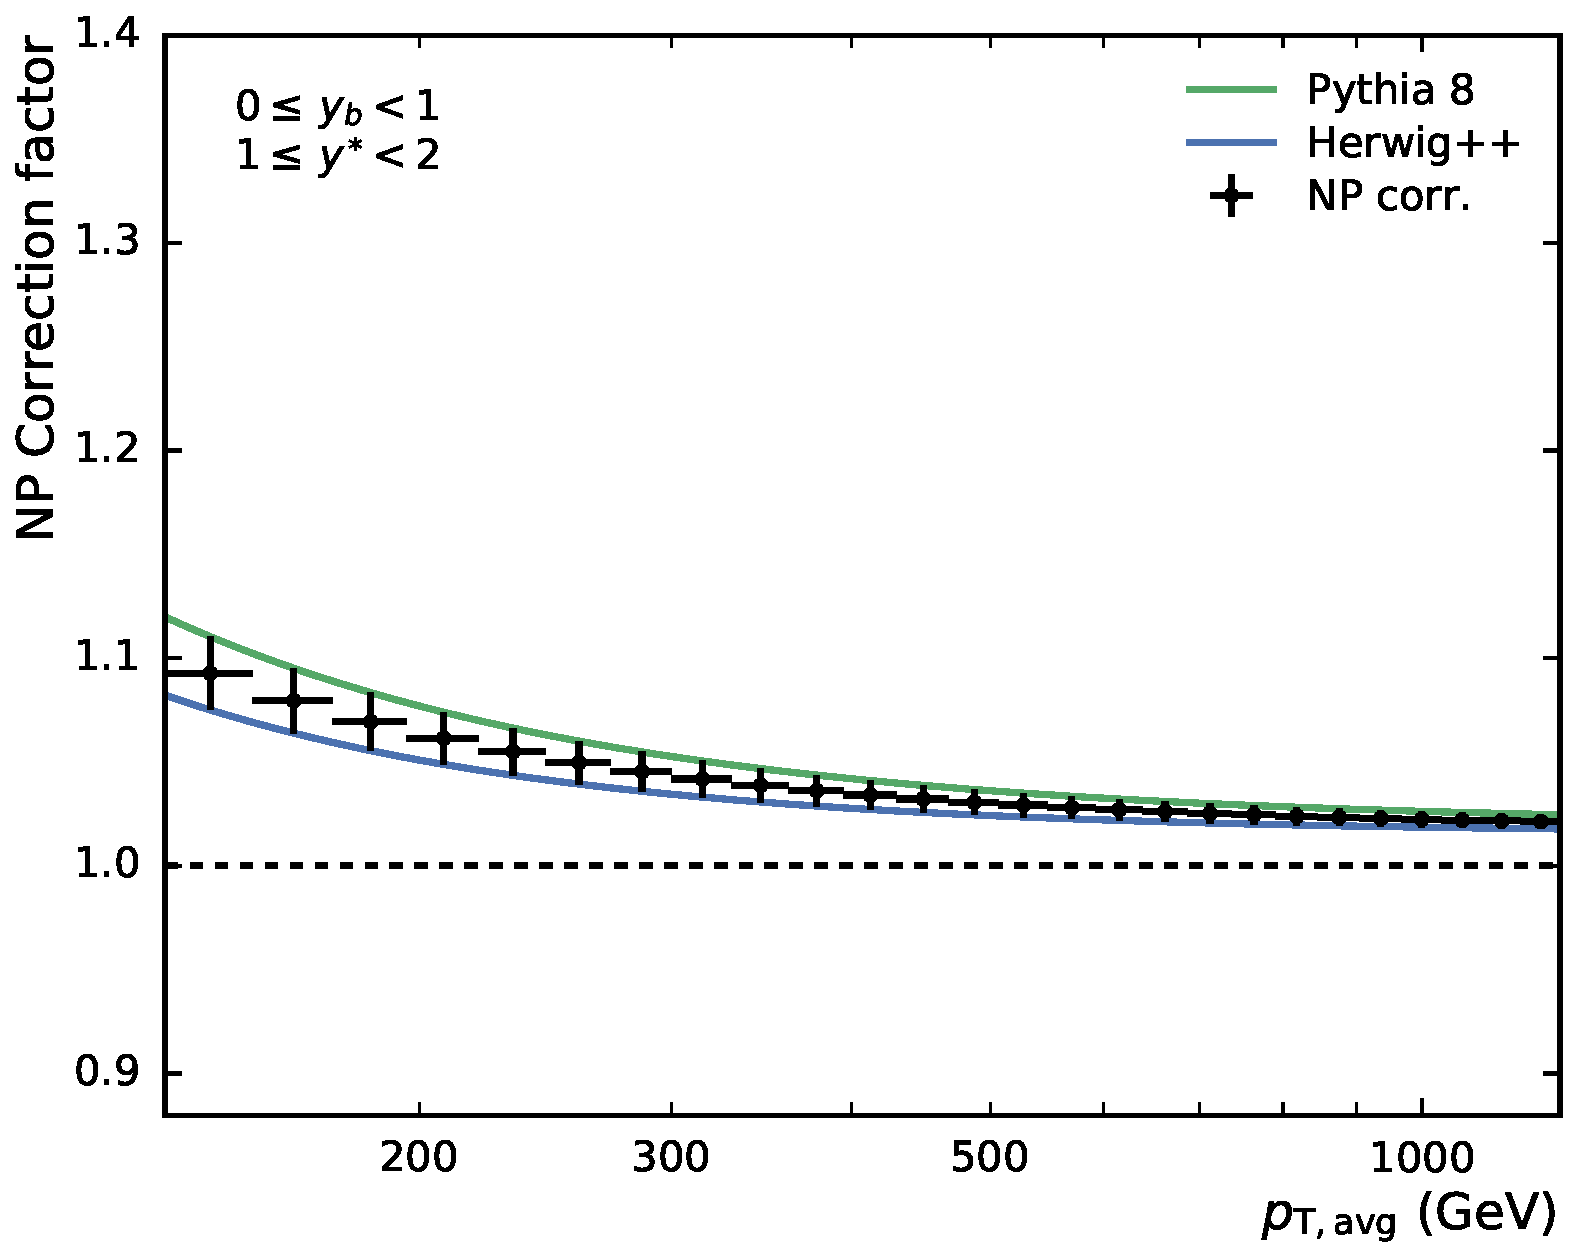
\includegraphics[width=0.45\textwidth]{figures/theory/np_factors_calc_yb0ys1.pdf}
    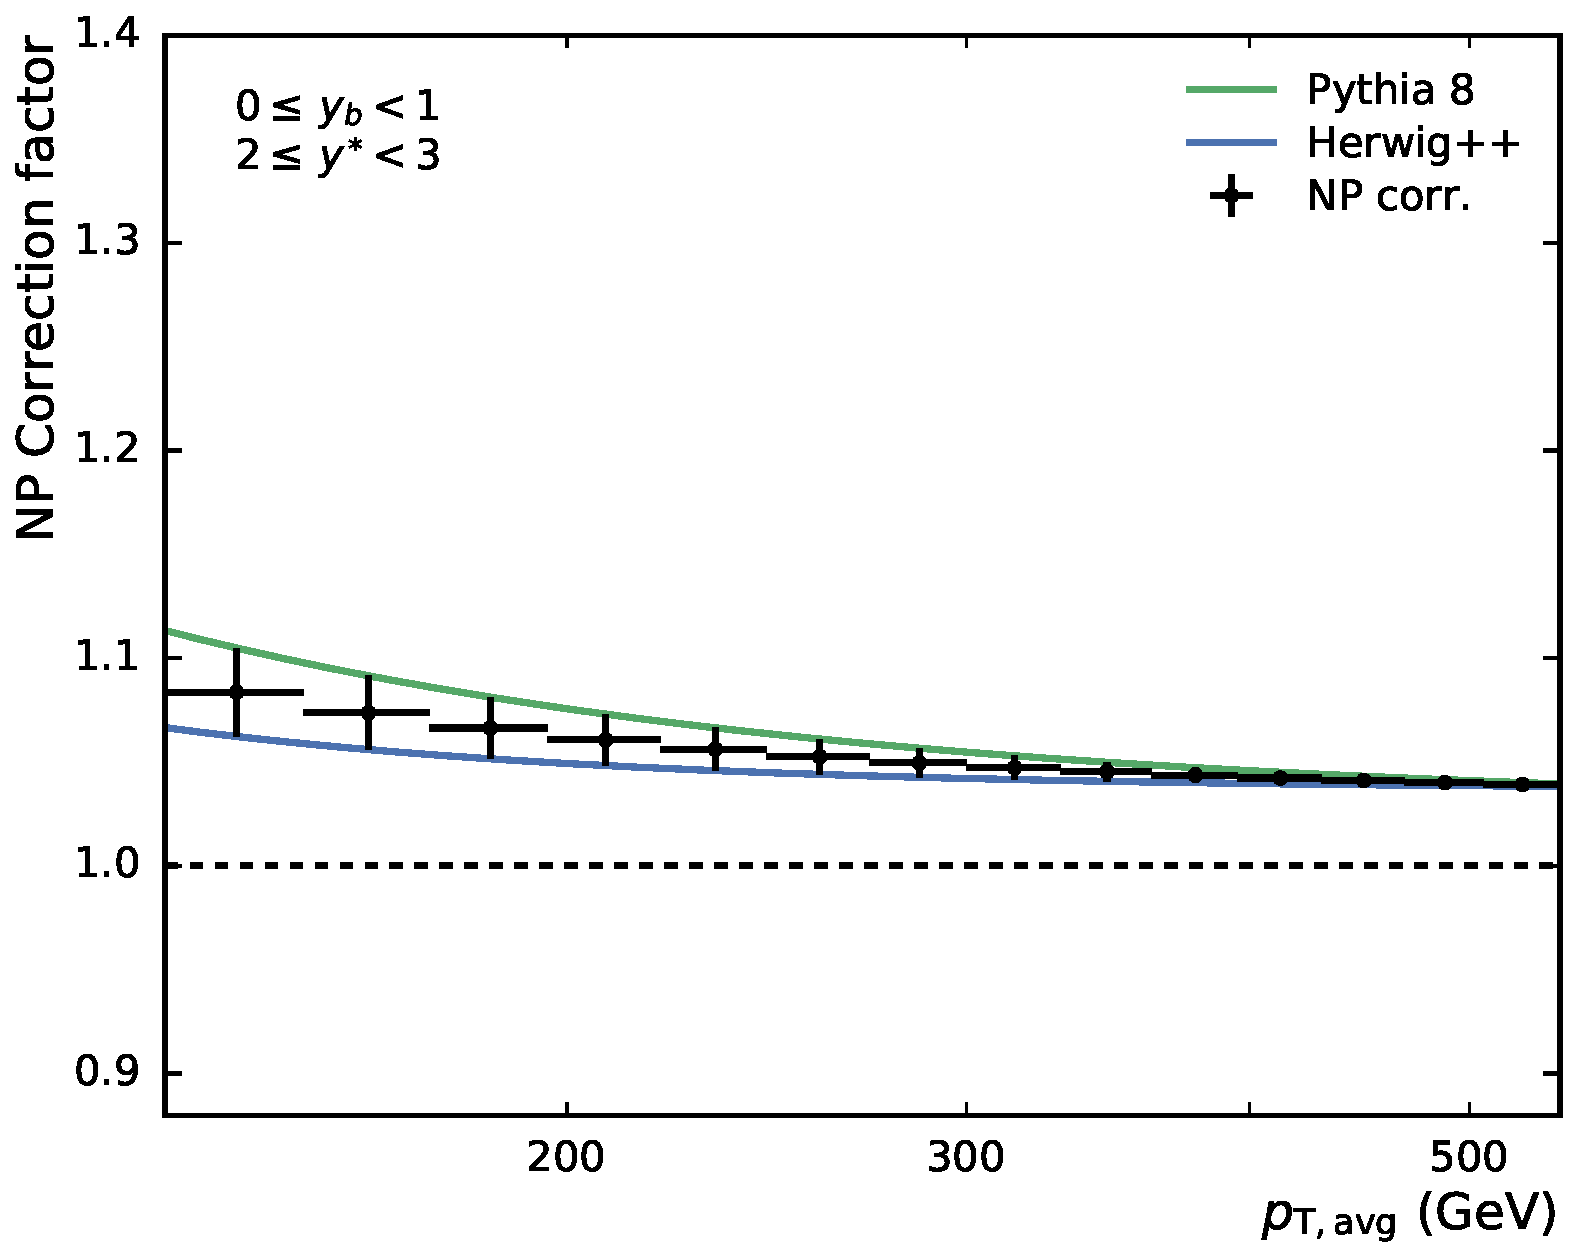
\includegraphics[width=0.45\textwidth]{figures/theory/np_factors_calc_yb0ys2.pdf}\hfill
    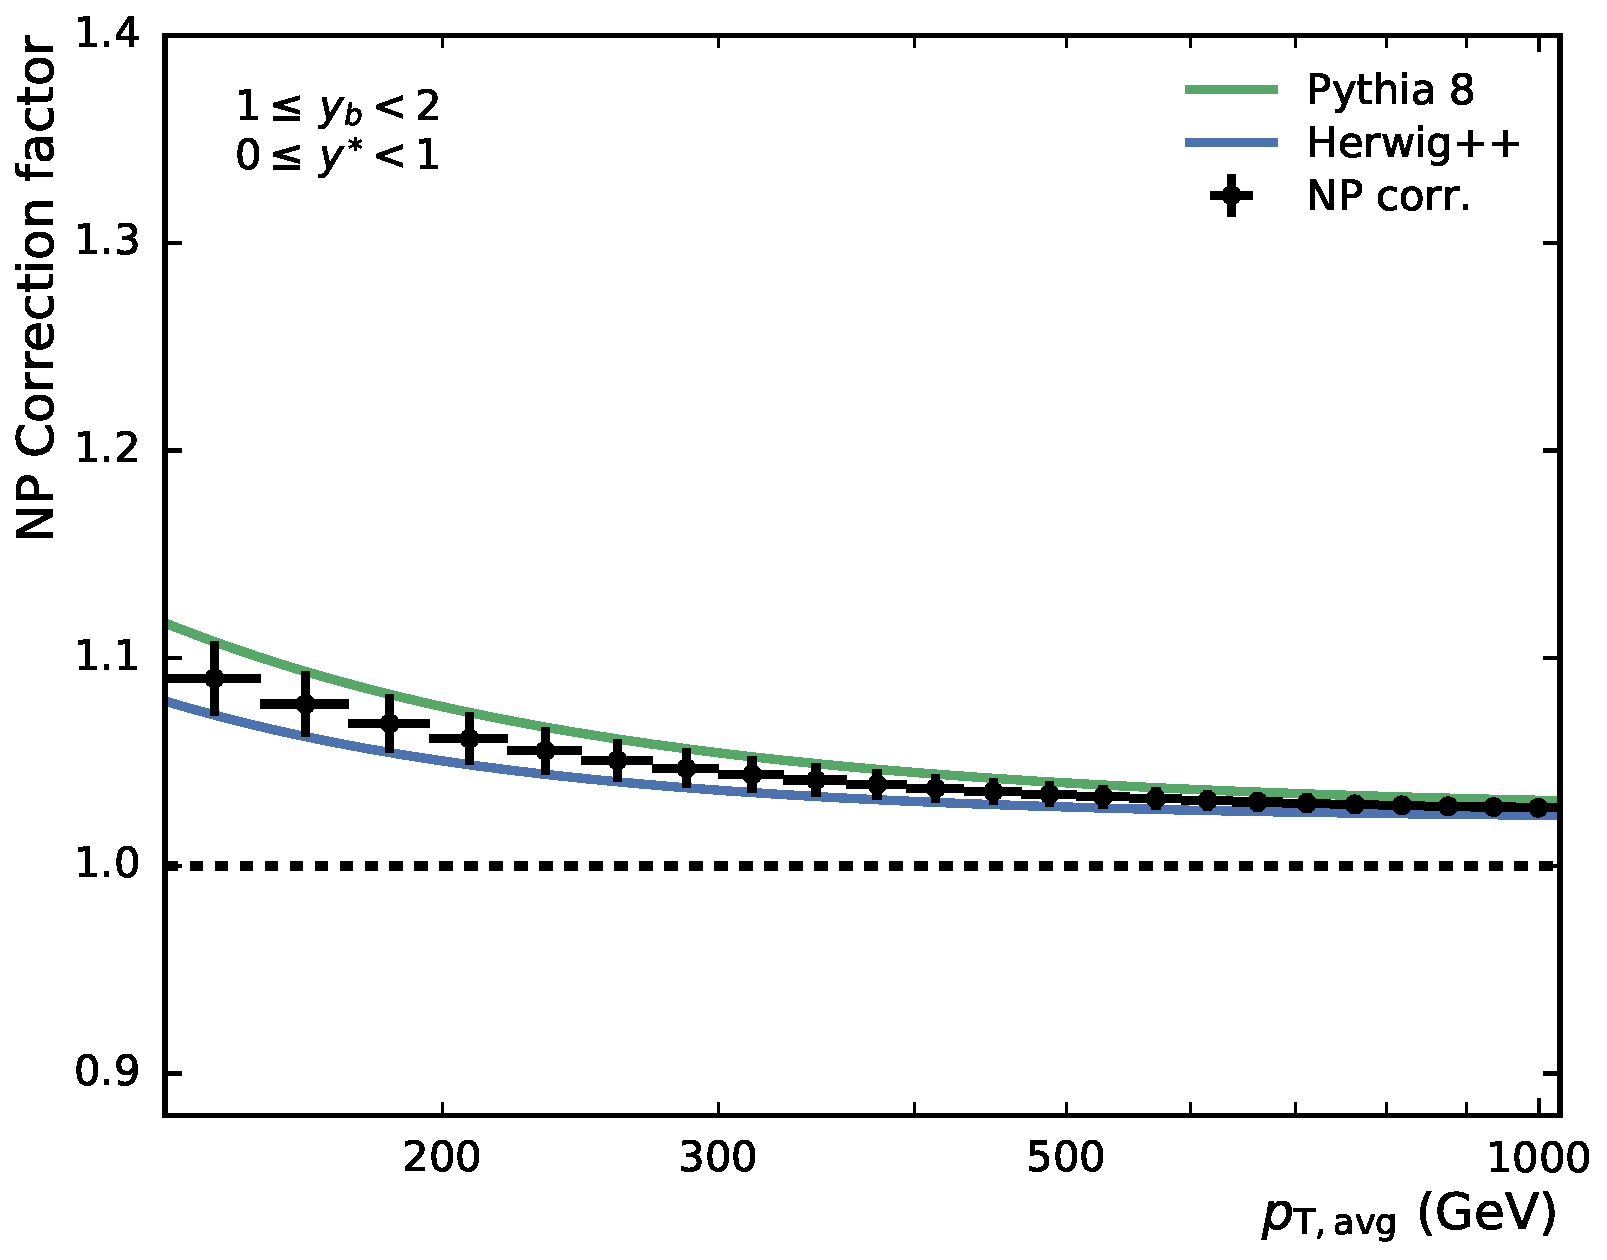
\includegraphics[width=0.45\textwidth]{figures/theory/np_factors_calc_yb1ys0.pdf}
    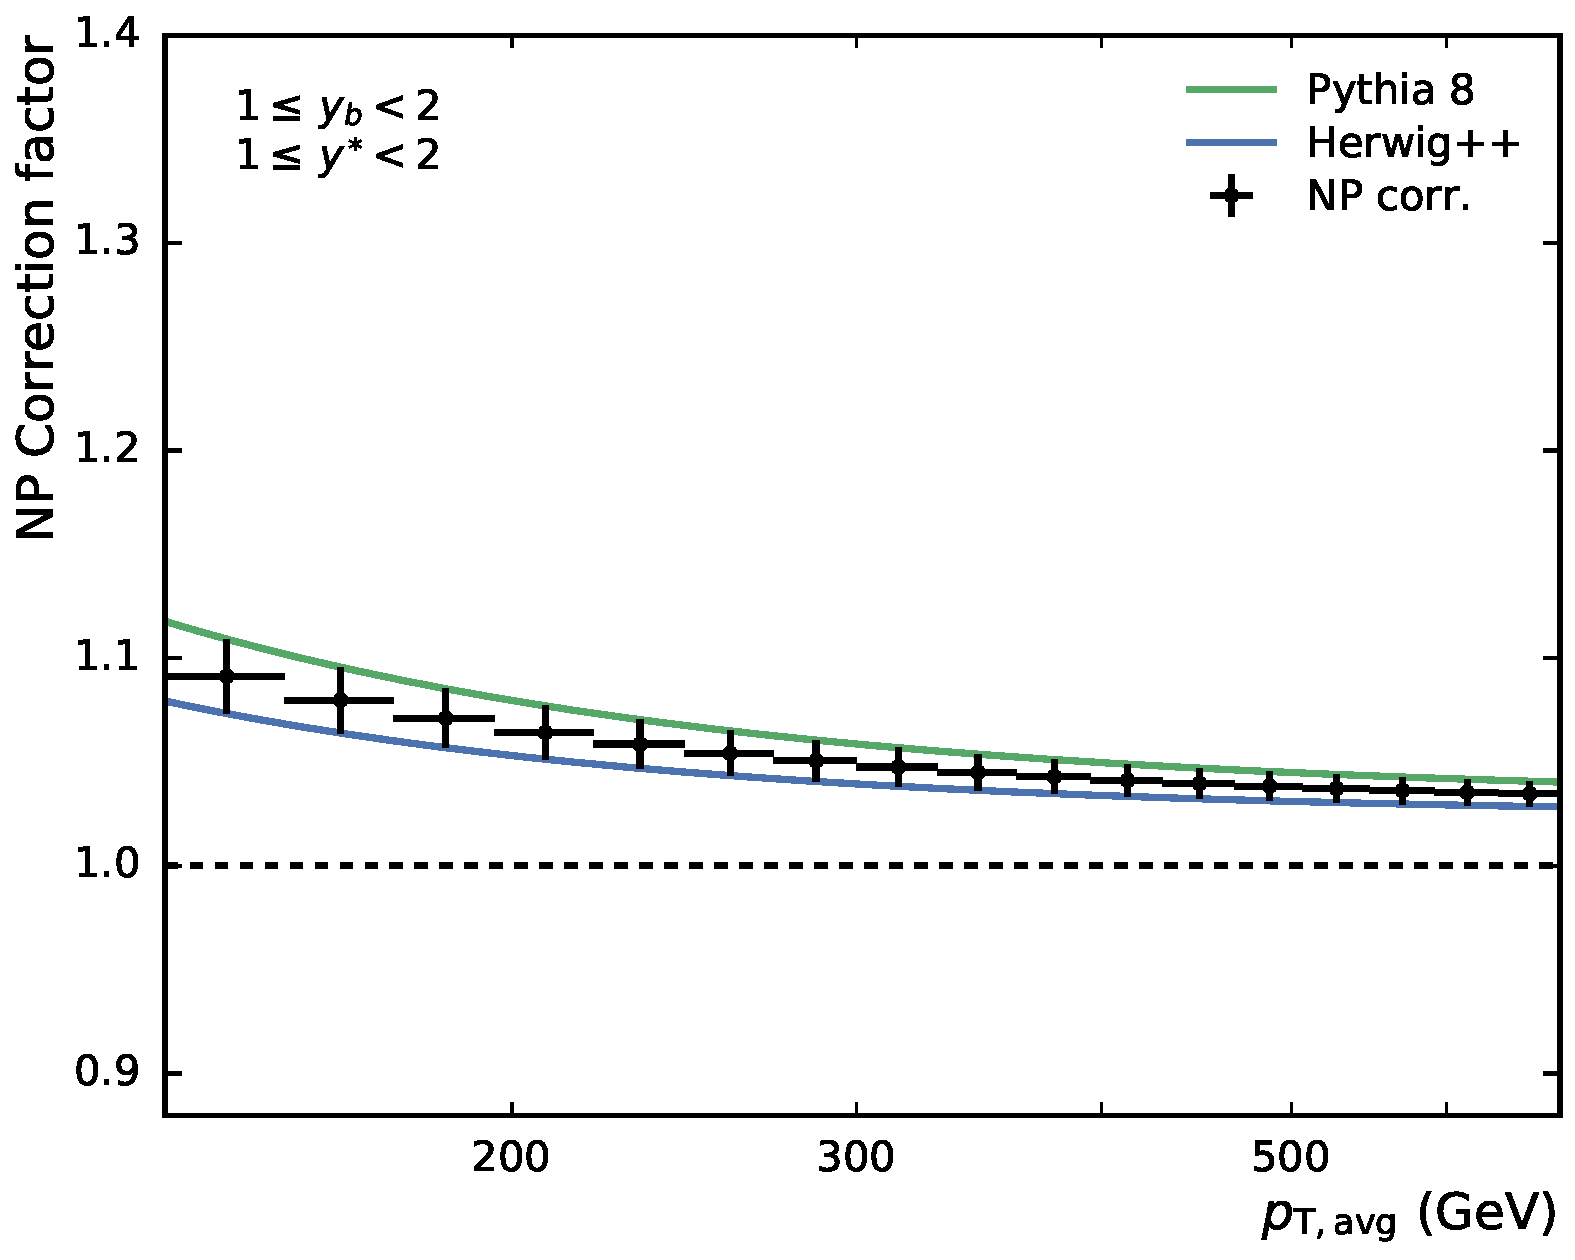
\includegraphics[width=0.45\textwidth]{figures/theory/np_factors_calc_yb1ys1.pdf}\hfill
    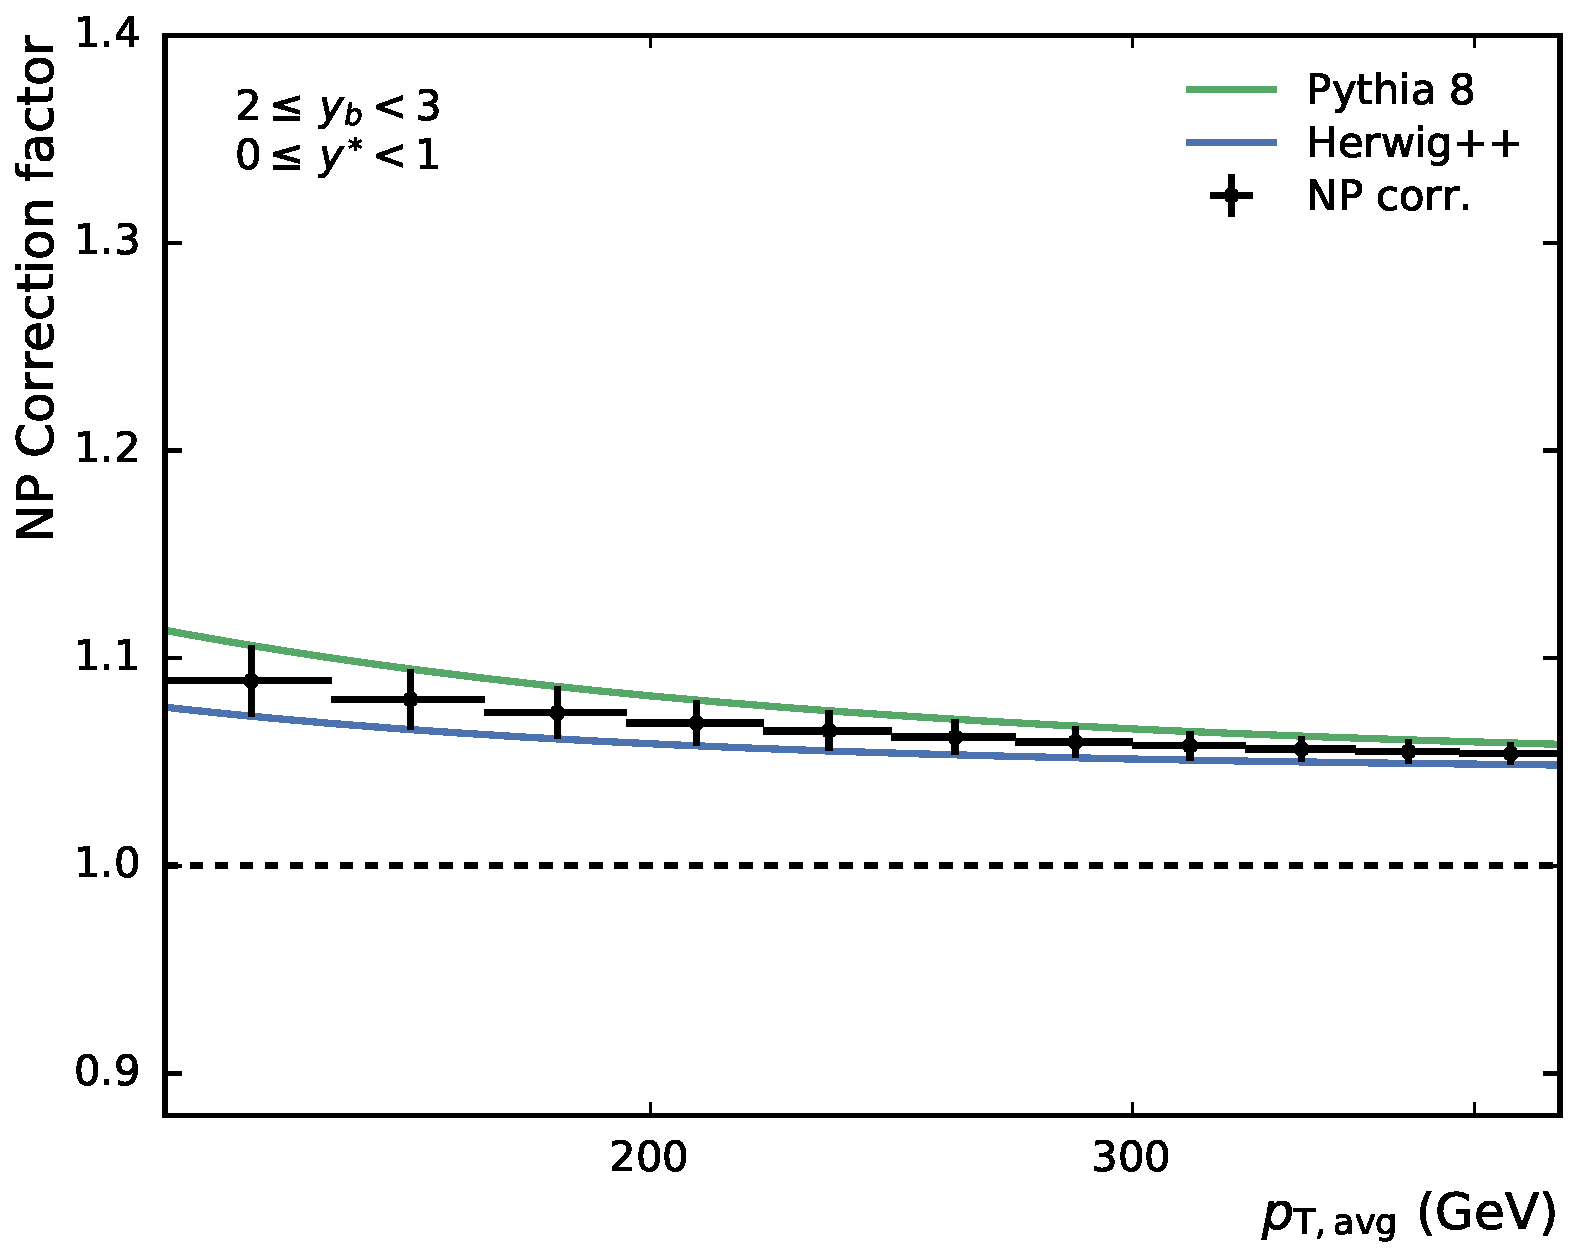
\includegraphics[width=0.45\textwidth]{figures/theory/np_factors_calc_yb2ys0.pdf}
    \caption{The non-perturbative correction is derived using a MC event
        generator by calculating the diferences by including hadronization and
        MPI in the simulation. The green line shows the correction of Pythia 8,
        the blue line the correction of Herwig++. The average of both gives the
        central correction and the envelope the uncertainty on the correction.}
    \label{fig:np_factors}
\end{figure}

\section{Theory Uncertainties}

Four sources of uncertainty limit the precision of the NLO theory preidction.
Thi section describes the derivation of the scale, PDF, \as and NP
uncertainties. Depending on the phasespace region the PDF or scale uncertainty
is the dominant source of uncertainty. The fastNLO table is
constructed from statistically independent calculations which are merged to
yield a high number of events. By estimating the uncertainty on the arithmetic
mean of all tables, the statistical uncertainty is found to be smaller than 0.5
\% in all bins, in most of the bins even smaller than 0.1 \%. Therefore the
statistical uncertainty was neglected in all further comparisons.

\subsection{Scale uncertainties}

Within the perturbative cross section calculations, one has to choose a
factorization and renormalization scale. The influence of these scales vanishes
when the calculation is performed for all orders of the perturbative series.
However since we truncate the series at NLO, a scale dependence on our result is
introduced. 

While the choice of the scale $\mu$ is per se arbitrary, it should reflect the
energy scale of the interaction. 

There is common approach in estimating the influence of the scale on the cross
section. The cross section calculation is performed using different scale
choices and the differences to the central scale choice is translated into an
uncertainty, called scale uncertainty. The variations are applied as relative
factors to the central choice in the following six combinations: $(\mur, \muf) =
(\sfrac{1}{2}, \sfrac{1}{2}), (\sfrac{1}{2}, 1), (1, \sfrac{1}{2}), (1, 2), (2,
1)$ and $(2, 2)$. The uncertainty is the envelope of the maximum deviation in
the upwards and downwards direction.  Fig.~\ref{fig:theo_uncertainties} shows
the relative size of the scale uncertainty for each of the measurement bins.

\begin{figure}[htp]
    \centering
    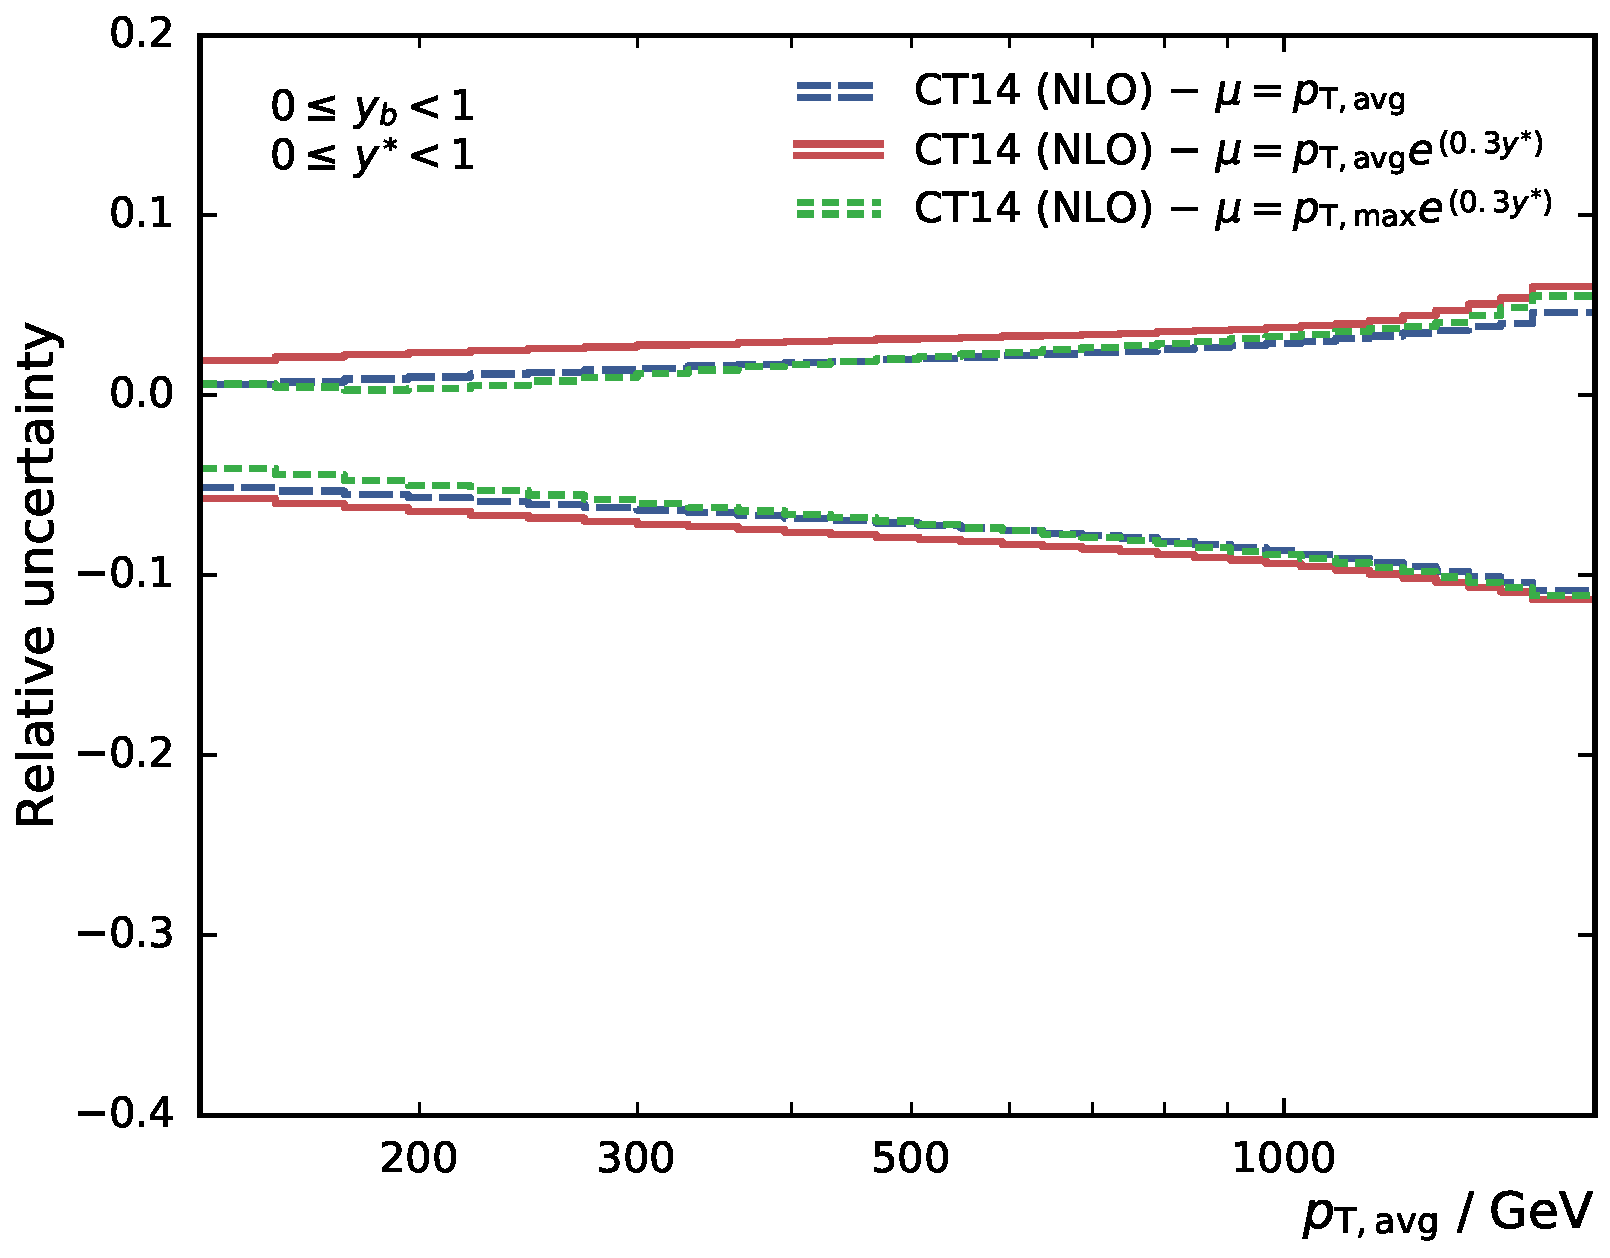
\includegraphics[width=0.45\textwidth]{figures/theory/scale_uncert_comp_yb0ys0.pdf}\hfill
    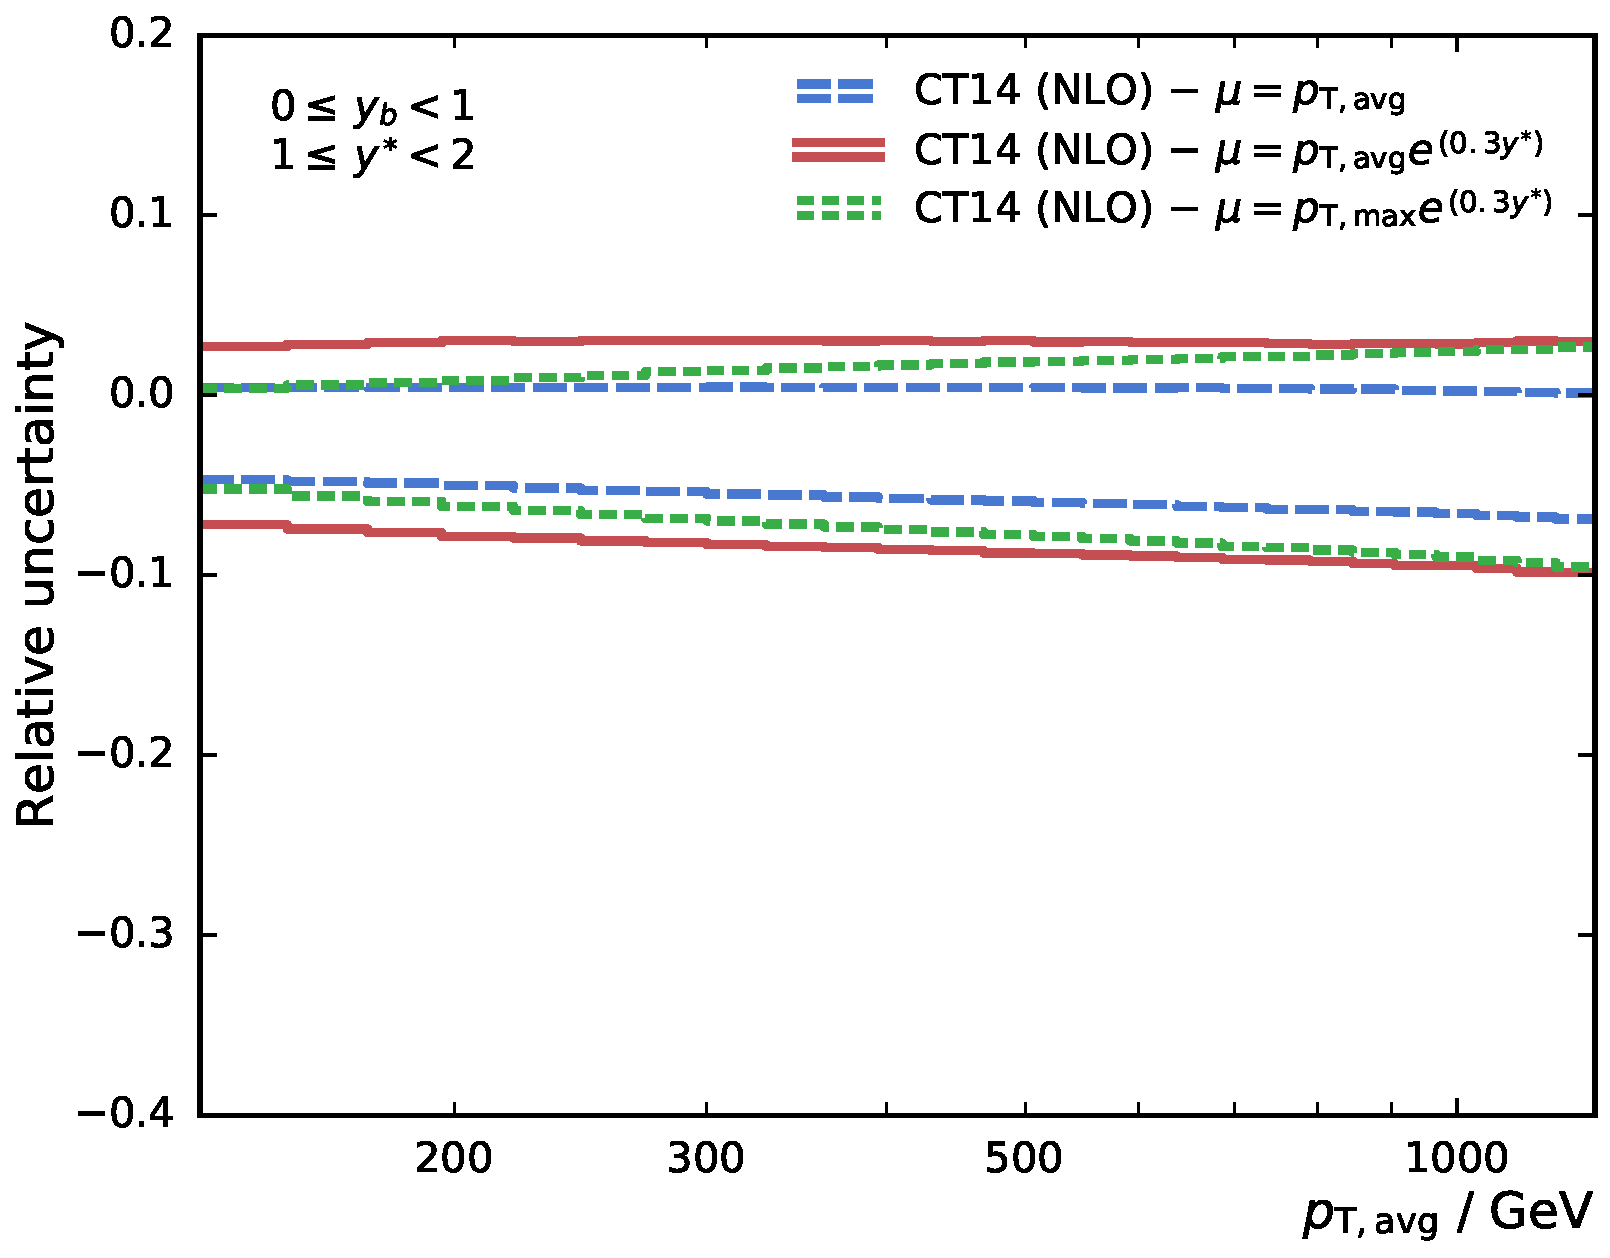
\includegraphics[width=0.45\textwidth]{figures/theory/scale_uncert_comp_yb0ys1.pdf}
    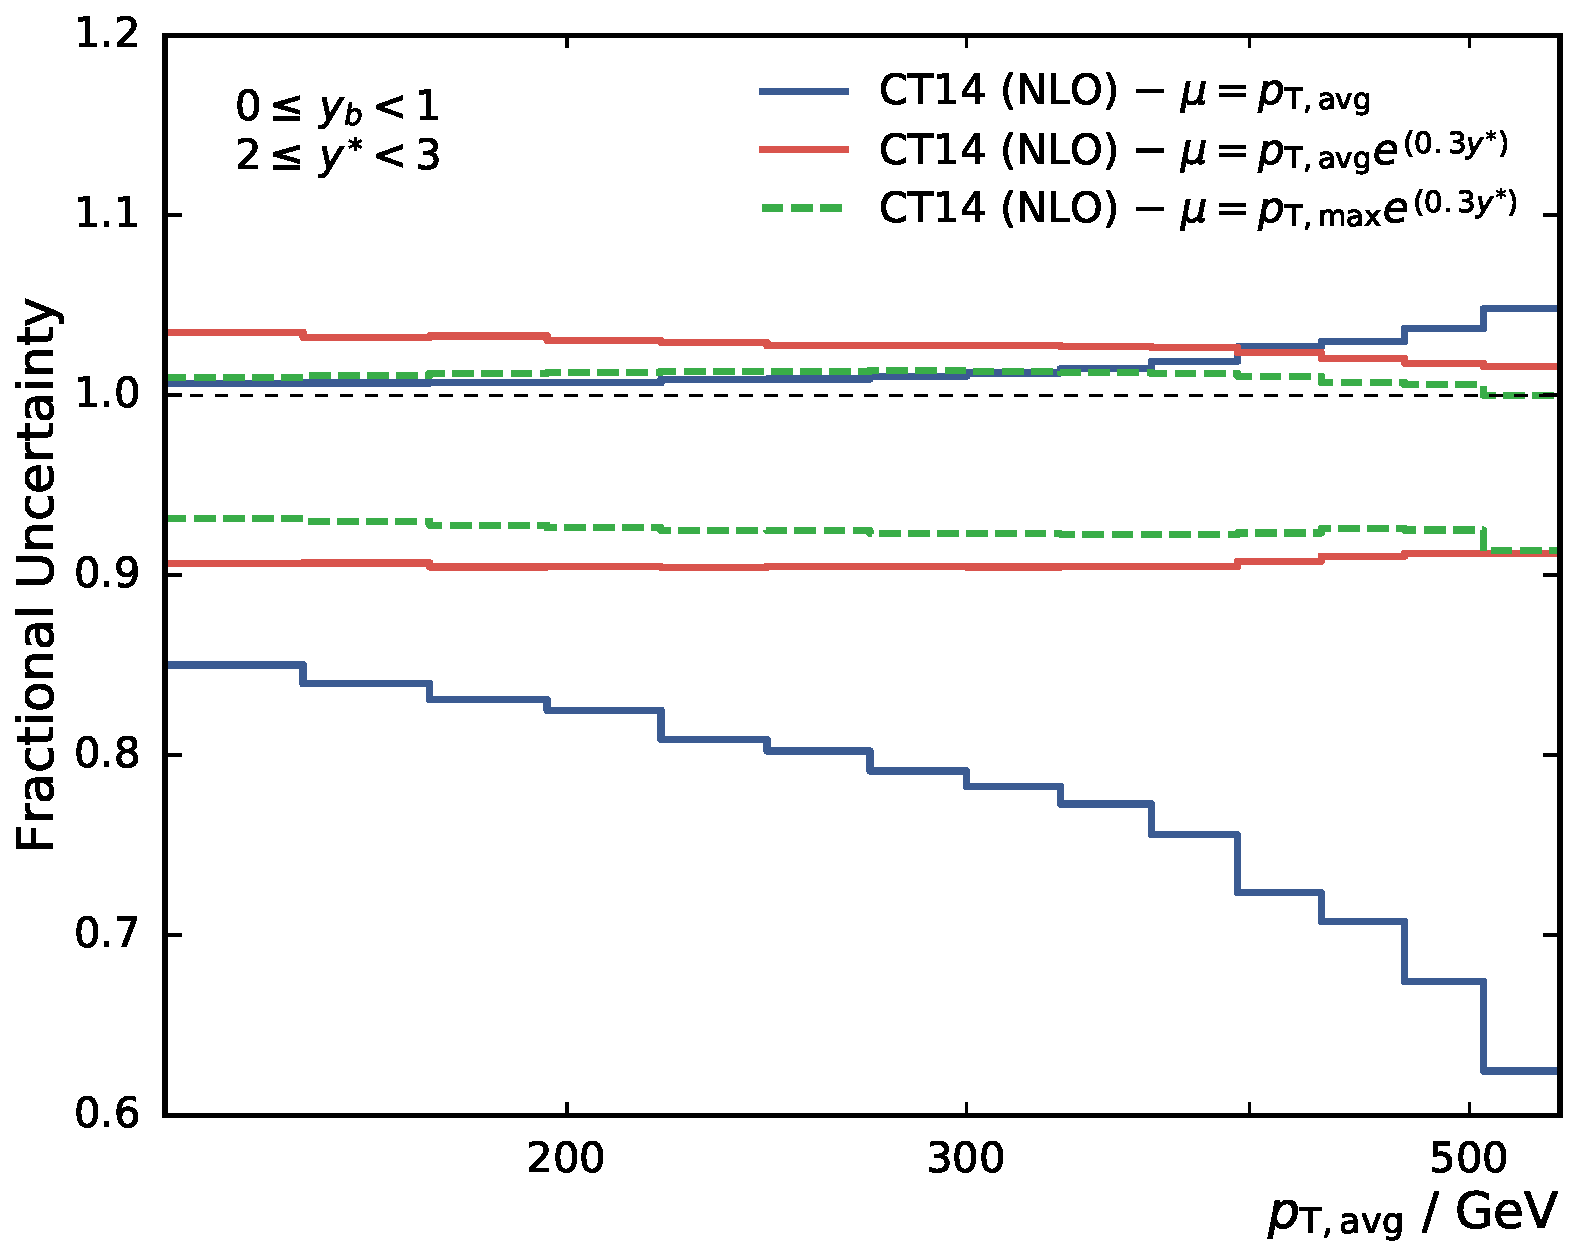
\includegraphics[width=0.45\textwidth]{figures/theory/scale_uncert_comp_yb0ys2.pdf}\hfill
    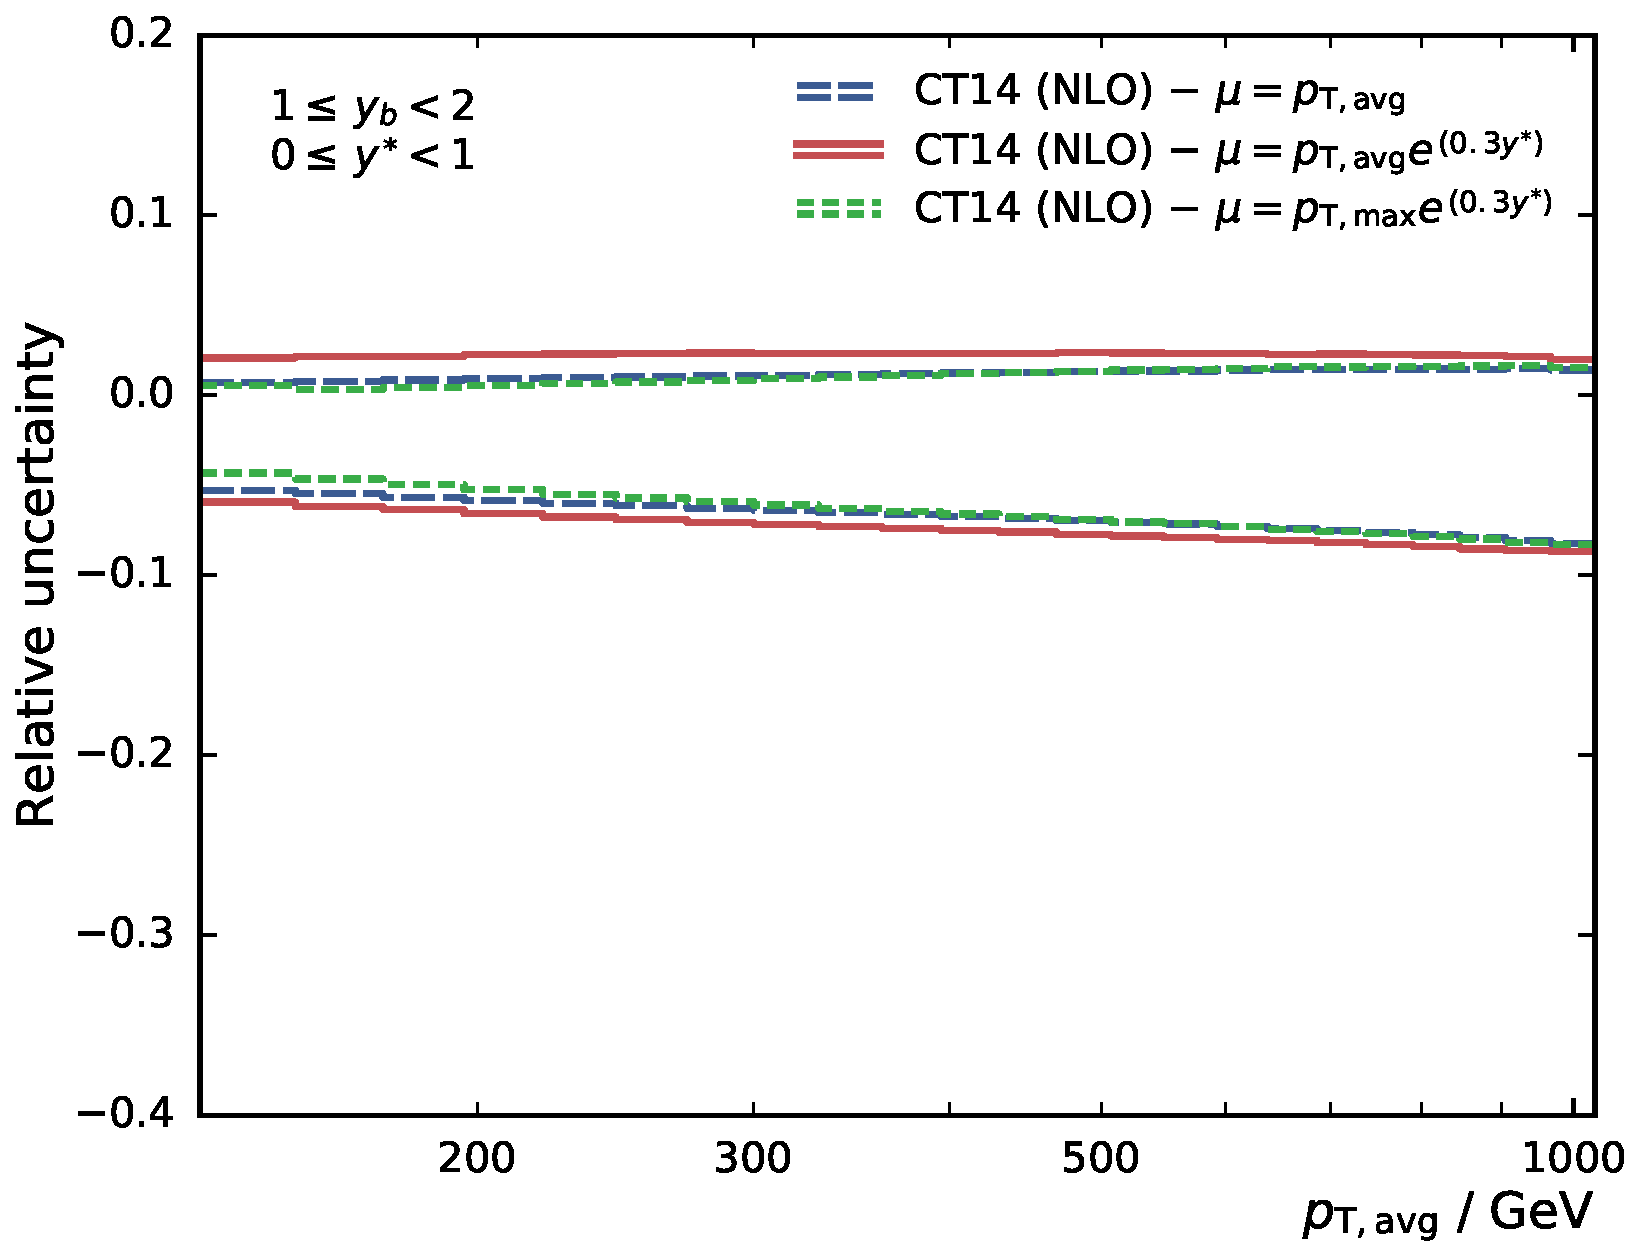
\includegraphics[width=0.45\textwidth]{figures/theory/scale_uncert_comp_yb1ys0.pdf}
    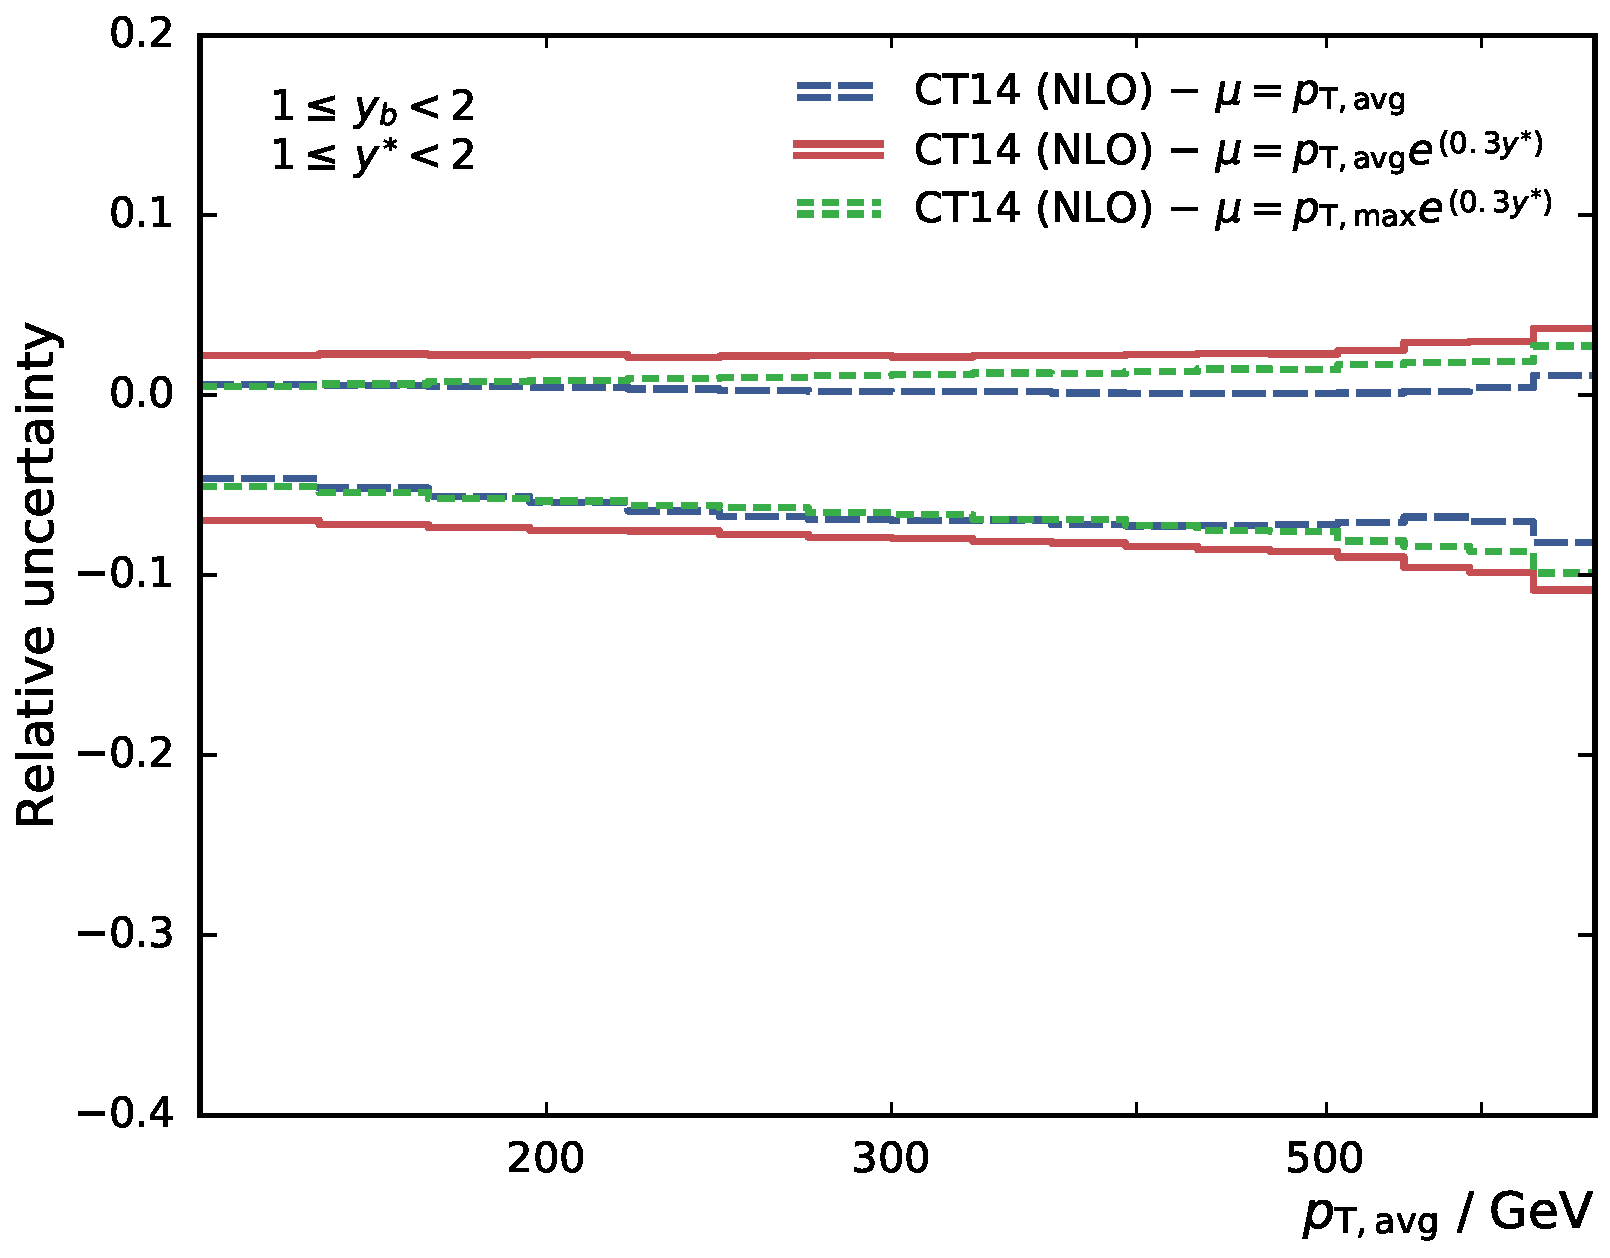
\includegraphics[width=0.45\textwidth]{figures/theory/scale_uncert_comp_yb1ys1.pdf}\hfill
    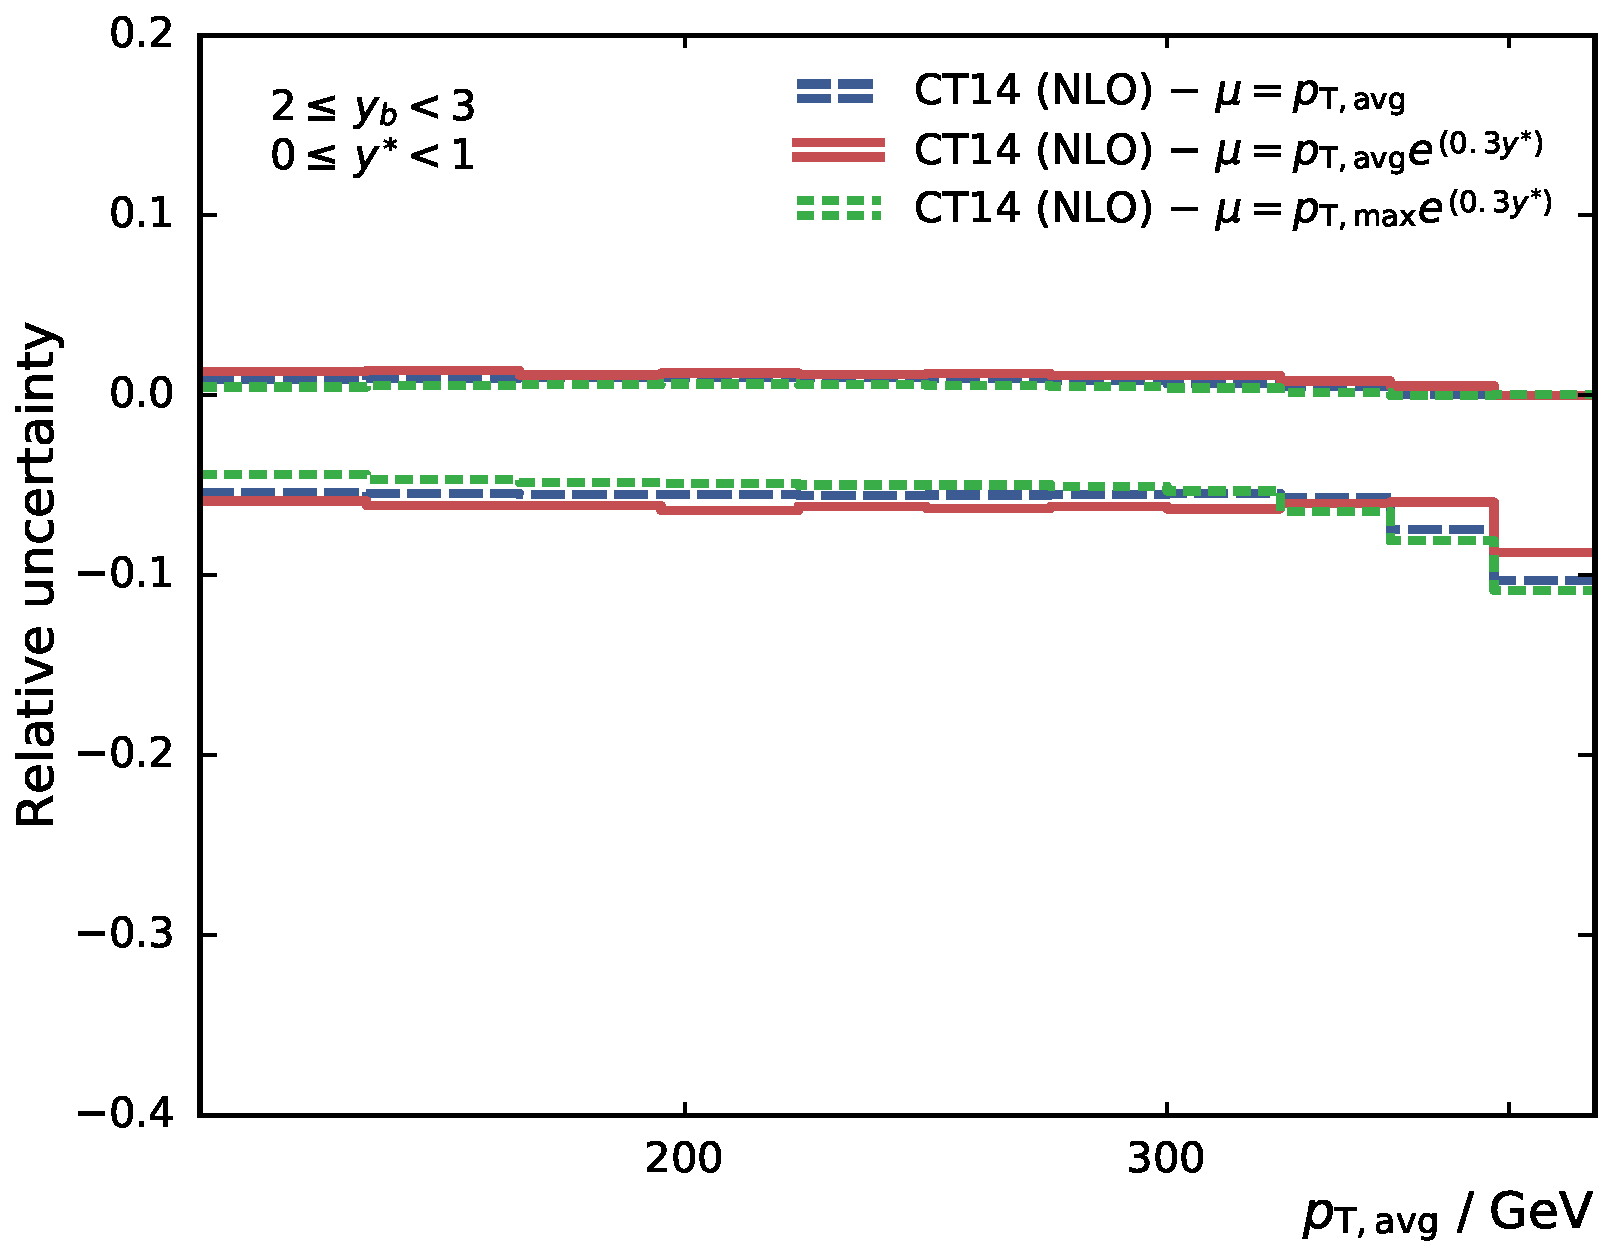
\includegraphics[width=0.45\textwidth]{figures/theory/scale_uncert_comp_yb2ys0.pdf}
    \caption{The scale uncertainty is estimated using the common approach of
        independently varying the renormalization and factorization scale
        choice in six independent combinations. The uncertainty is shown for the
        three investigated scale choices. In most cases the scale uncertainty is
        reasonable and of the size of 5\% to 10\%. In the high \ystar bin, the
        scale uncertainty of prediction with the \ptavg scale choice is
        undesirable large.}
    \label{fig:scale_uncertainties}
\end{figure}

\subsection{PDF uncertainties}

The dependence of the cross section calculation on the proton structure is
expressed in terms of parton distribution functions, which are derived from a
fit to data from different experiments. There are different sources of
uncertainty introduced when deriving the PDFs. These include the choice and the
functional form of the parametrization, the chosen theory model and input
parameters like the strong coupling or the quark masses as well as the data
uncertainties which are propagated onto the PDFs.

There derivation of PDF uncertainties follows prescriptions of each individual
PDF set. The NNPDF PDF sets use Monte-Carlo pseudoexperiments, in which the PDF
fit is performed using data smeared within their uncertainties taking into
account the correlations. These so-called replicas are then averaged to give the
central result and the spread of the replicas determines the uncertainty. The
PDF uncertainty of a quantity $X$ which can be a cross section calculation or
even the PDF itself is expressed as

\begin{equation*}
    \Delta X = \sqrt{\frac{1}{N-1} \sum_{i=1}^N \left( X_{i} - X_{\mathrm{central}} , 0 \right)^2}
\end{equation*}

The CT14 and MMHT PDF sets both employ the eigenvector method to encode the
uncertainties. A transformation from the parameter basis to the eigenvector
basis is done to yield mutually uncorrelated eigenvectors. By varying the
eigenvectors upwards and downwards, a set of eigenvector pairs is generated which can used to
determine the asymmetric uncertainty $X_+$ and $X_-$ of a quantity..

\begin{equation*}
\begin{aligned}
\Delta X^+ &= \sqrt{\sum_i^{N_{\mathrm{EV}}} \left[ \max(X_i^+ -X_0, X_i^- - X_0, 0)\right]^2}\\
\Delta X^- &= \sqrt{\sum_i^{N_{\mathrm{EV}}} \left[ \min(X_i^+ -X_0, X_i^- - X_0,0)\right]^2}
\end{aligned}
\end{equation*}

The symmetric uncertainty is given by half the difference of the upwards and
downwards variation.

\begin{equation*}
    \Delta X = \sqrt{\sum_i^{N_{\mathrm{EV}}} \left[ \frac{\left( X_i^+ -
    X_i^-\right)}{2} \right]^2}
\end{equation*}

The CT14 PDF uncertainties describe a 90\% confidence interval while the MMHT
and NNPDF PDF uncertainties represent a 68\% confidence interval. The CT14
uncertainties are scaled to 68CL using $s = \sqrt{2} \erf^{-1}(0.9) = 1.645$.
Fig.~\ref{fig:pdf_uncertainties} shows the fractional PDF uncertainty for
these three PDF sets. The PDF uncertainty in the bins with a small \ystar and a
small \yboost value is comparably small. This is due to the fact that mostly
events with two jets which are balanced in rapidity contribute. The PDF
uncertainty in the bin with high \ystar value and a low \yboost value, in which
two forward jets which are back-to-back in rapidity is similar and not sizeable.
The most interesting region is the one with a high \yboost value. There the
rapidity of both jets has the same sign and is large. To achieve this high boost, one
must access the high-$x$ region of one proton, which is not well known and is
afflicted with large PDF uncertainties. Especially the NNPDF PDF set has a large
uncertainty in this region. This is caused by the very flexible parametrization
of the NNPDF PDF set which results in large PDF uncertainty in phase space
regions not covered by data.

\begin{figure}[htp]
    \centering
    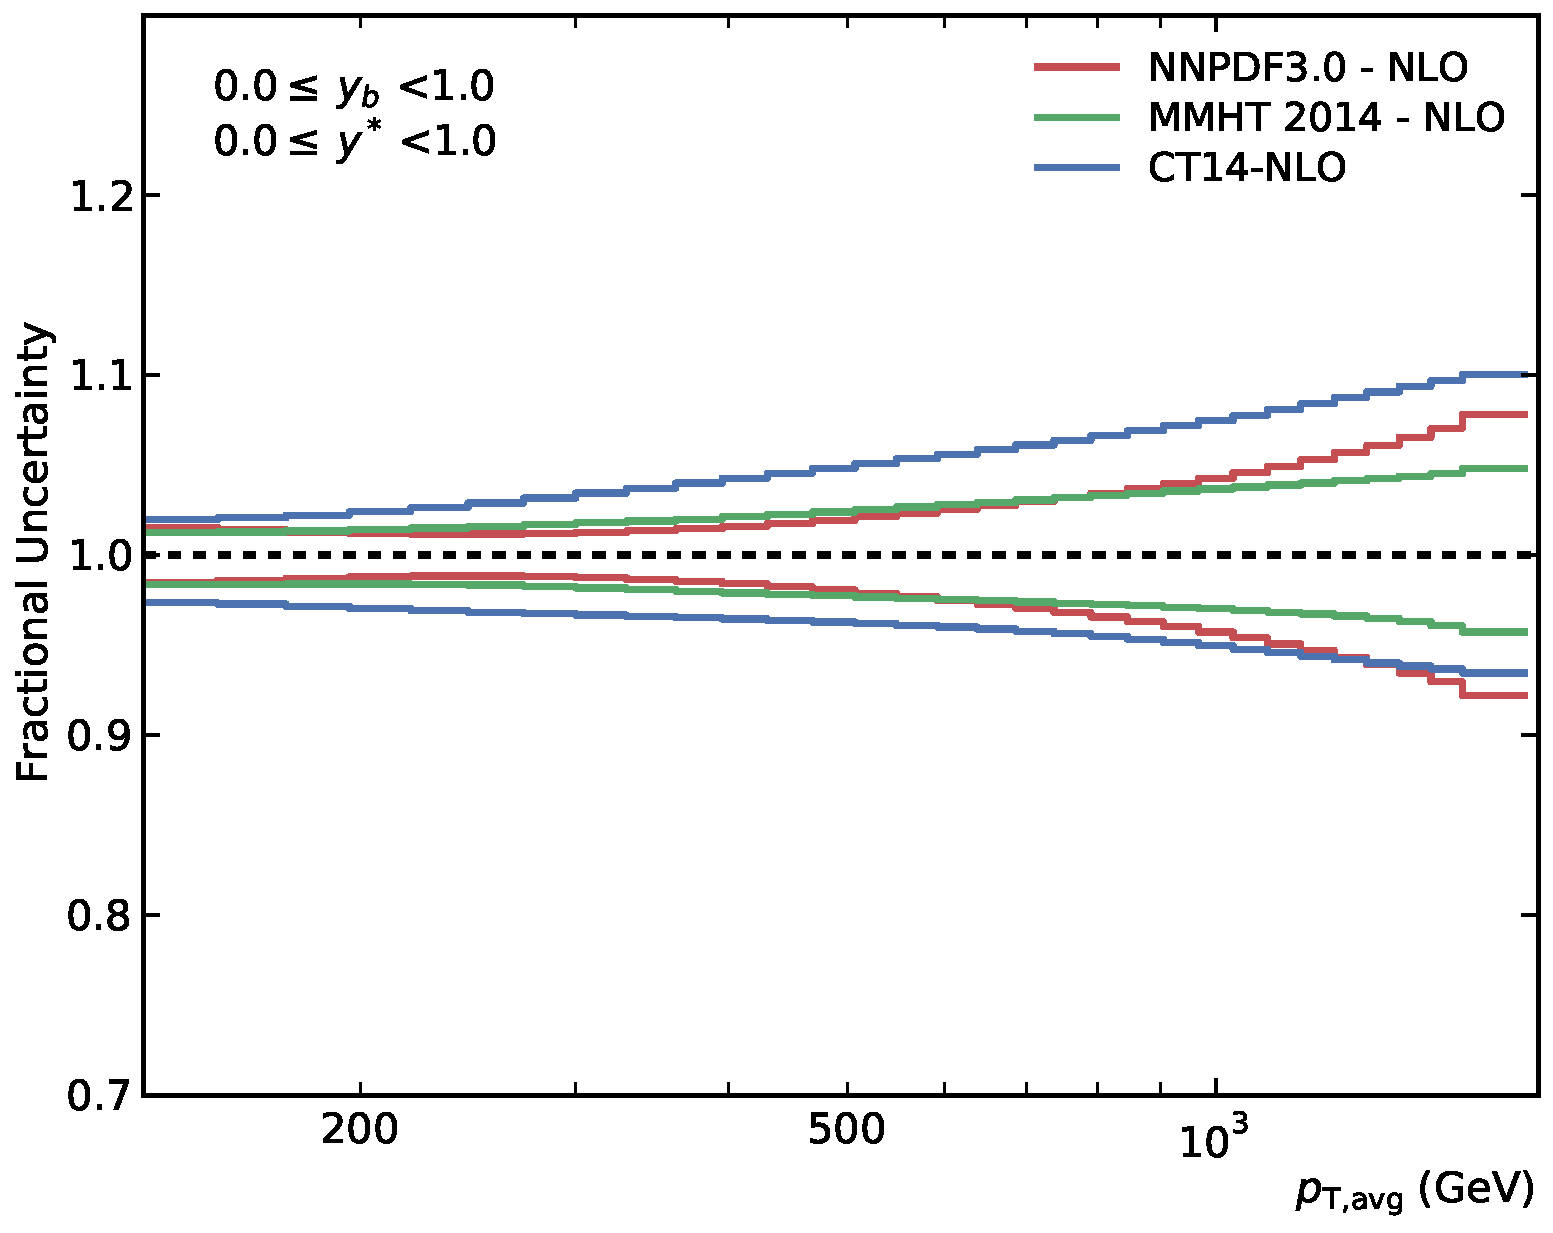
\includegraphics[width=0.45\textwidth]{figures/theory/pdf_unc_comparison_yb0ys0.pdf}\hfill
    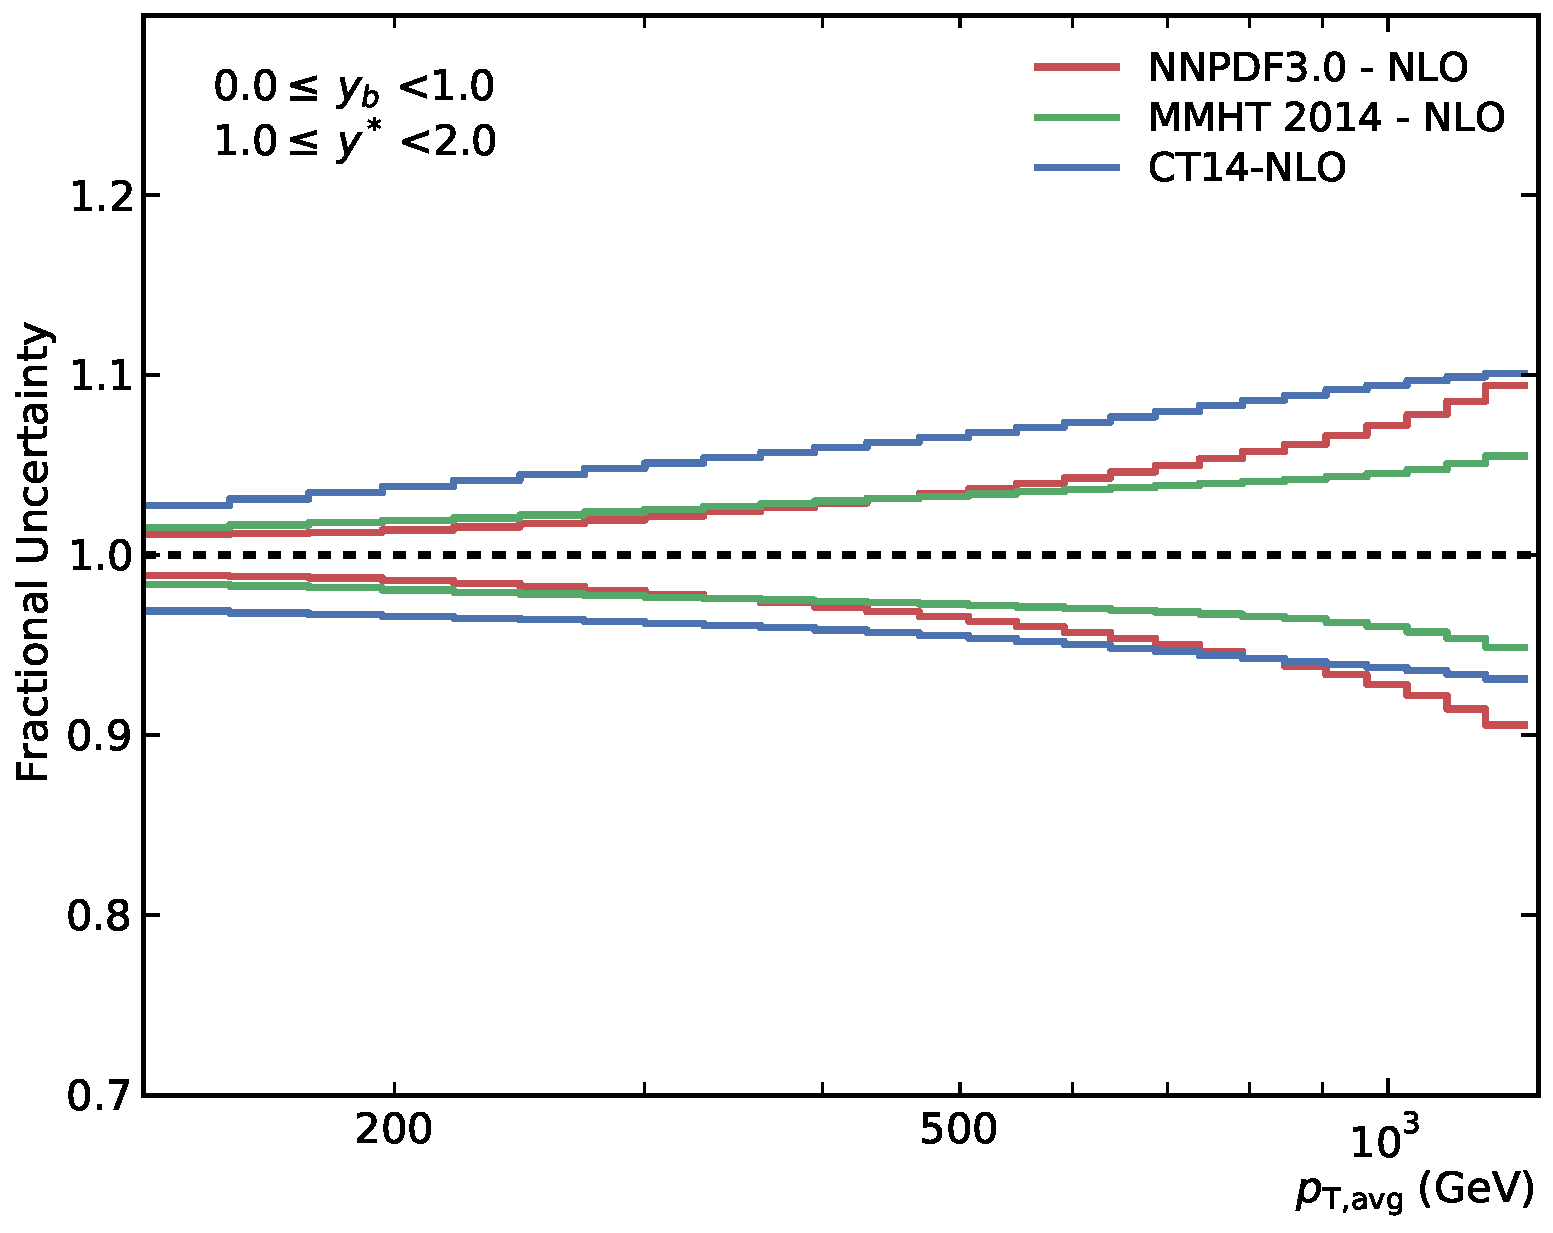
\includegraphics[width=0.45\textwidth]{figures/theory/pdf_unc_comparison_yb0ys1.pdf}
    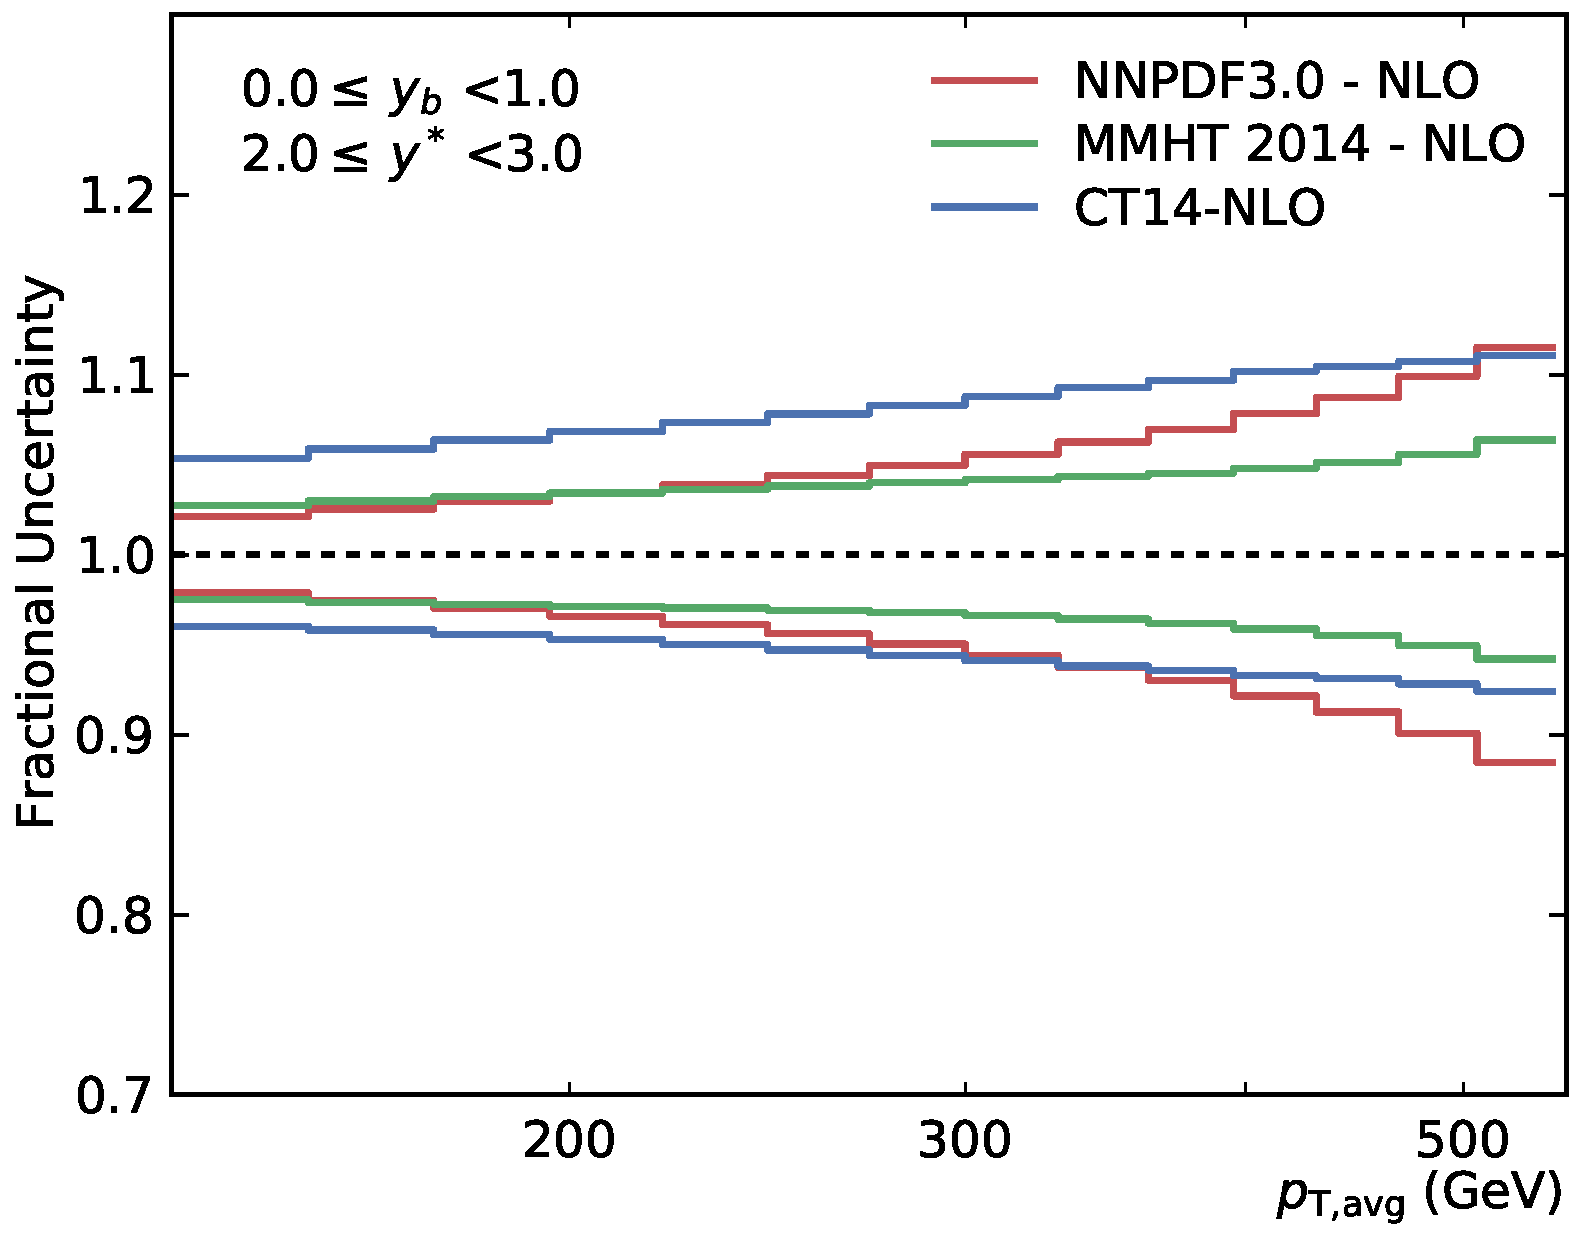
\includegraphics[width=0.45\textwidth]{figures/theory/pdf_unc_comparison_yb0ys2.pdf}\hfill
    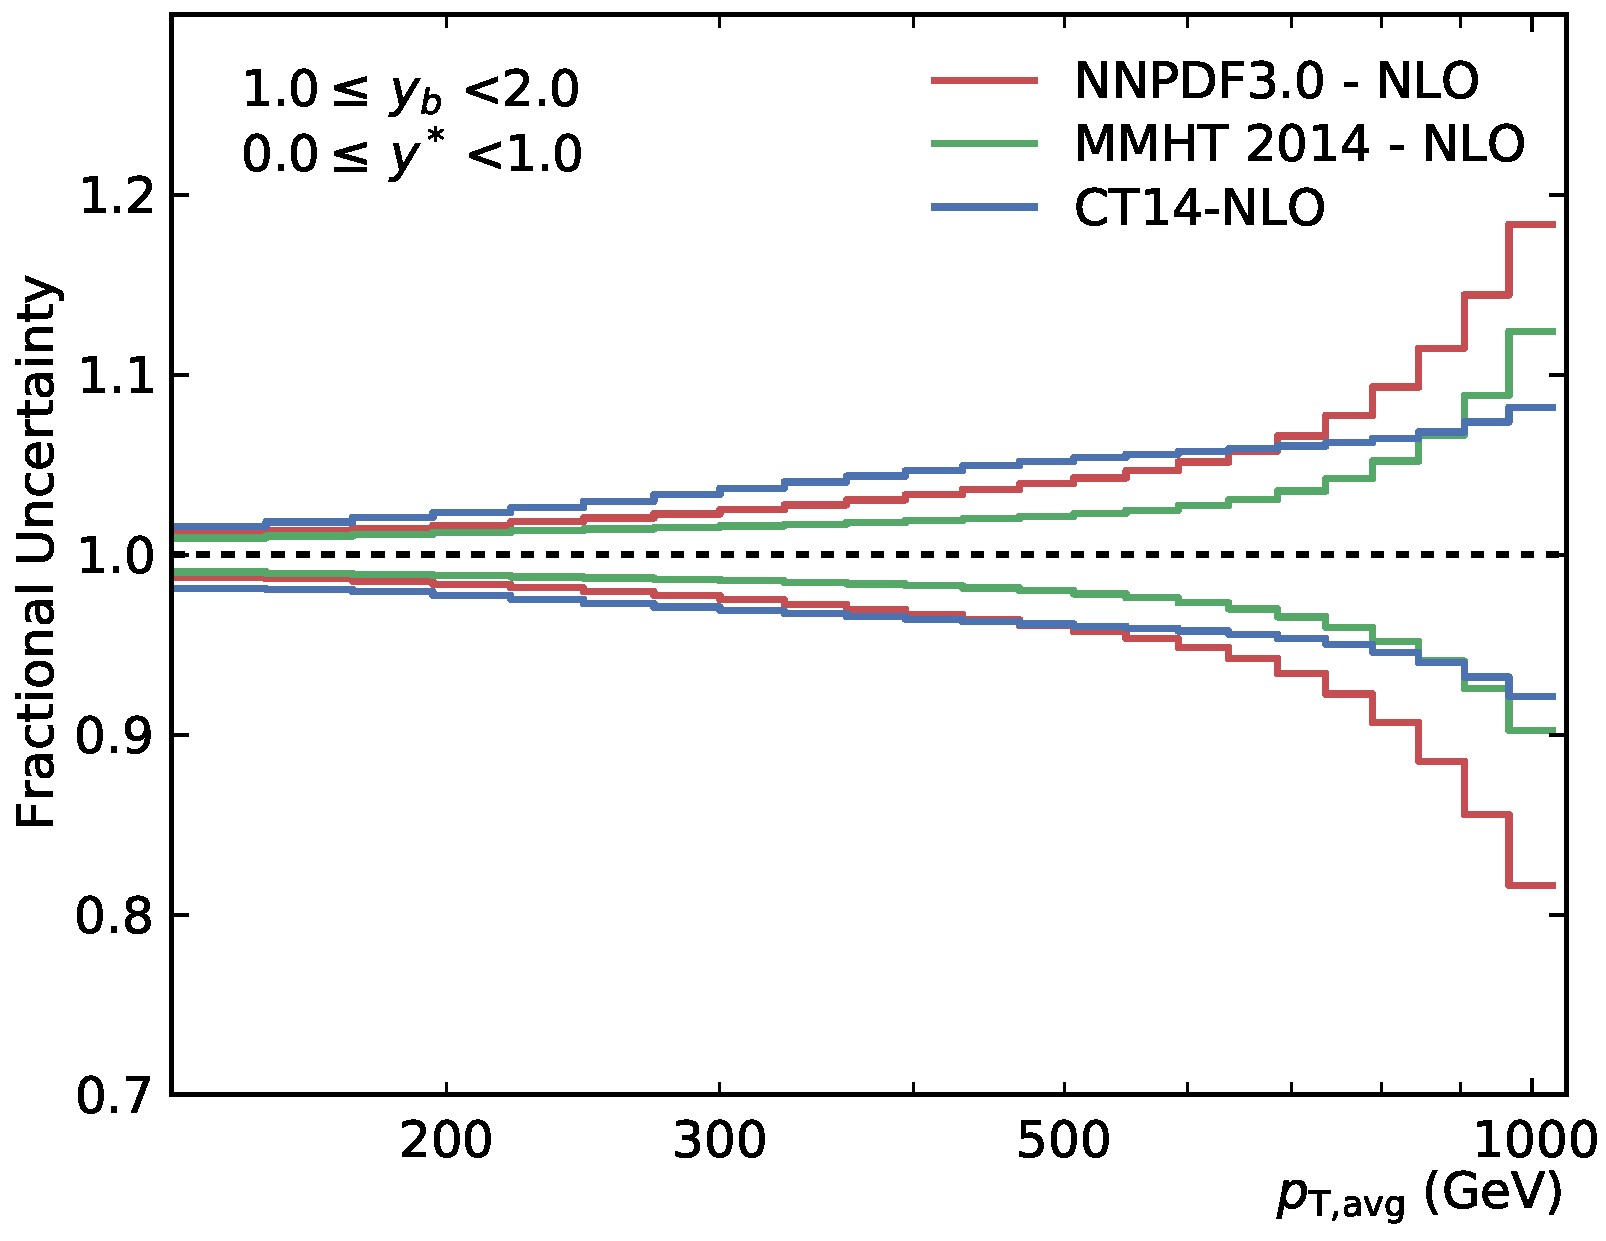
\includegraphics[width=0.45\textwidth]{figures/theory/pdf_unc_comparison_yb1ys0.pdf}
    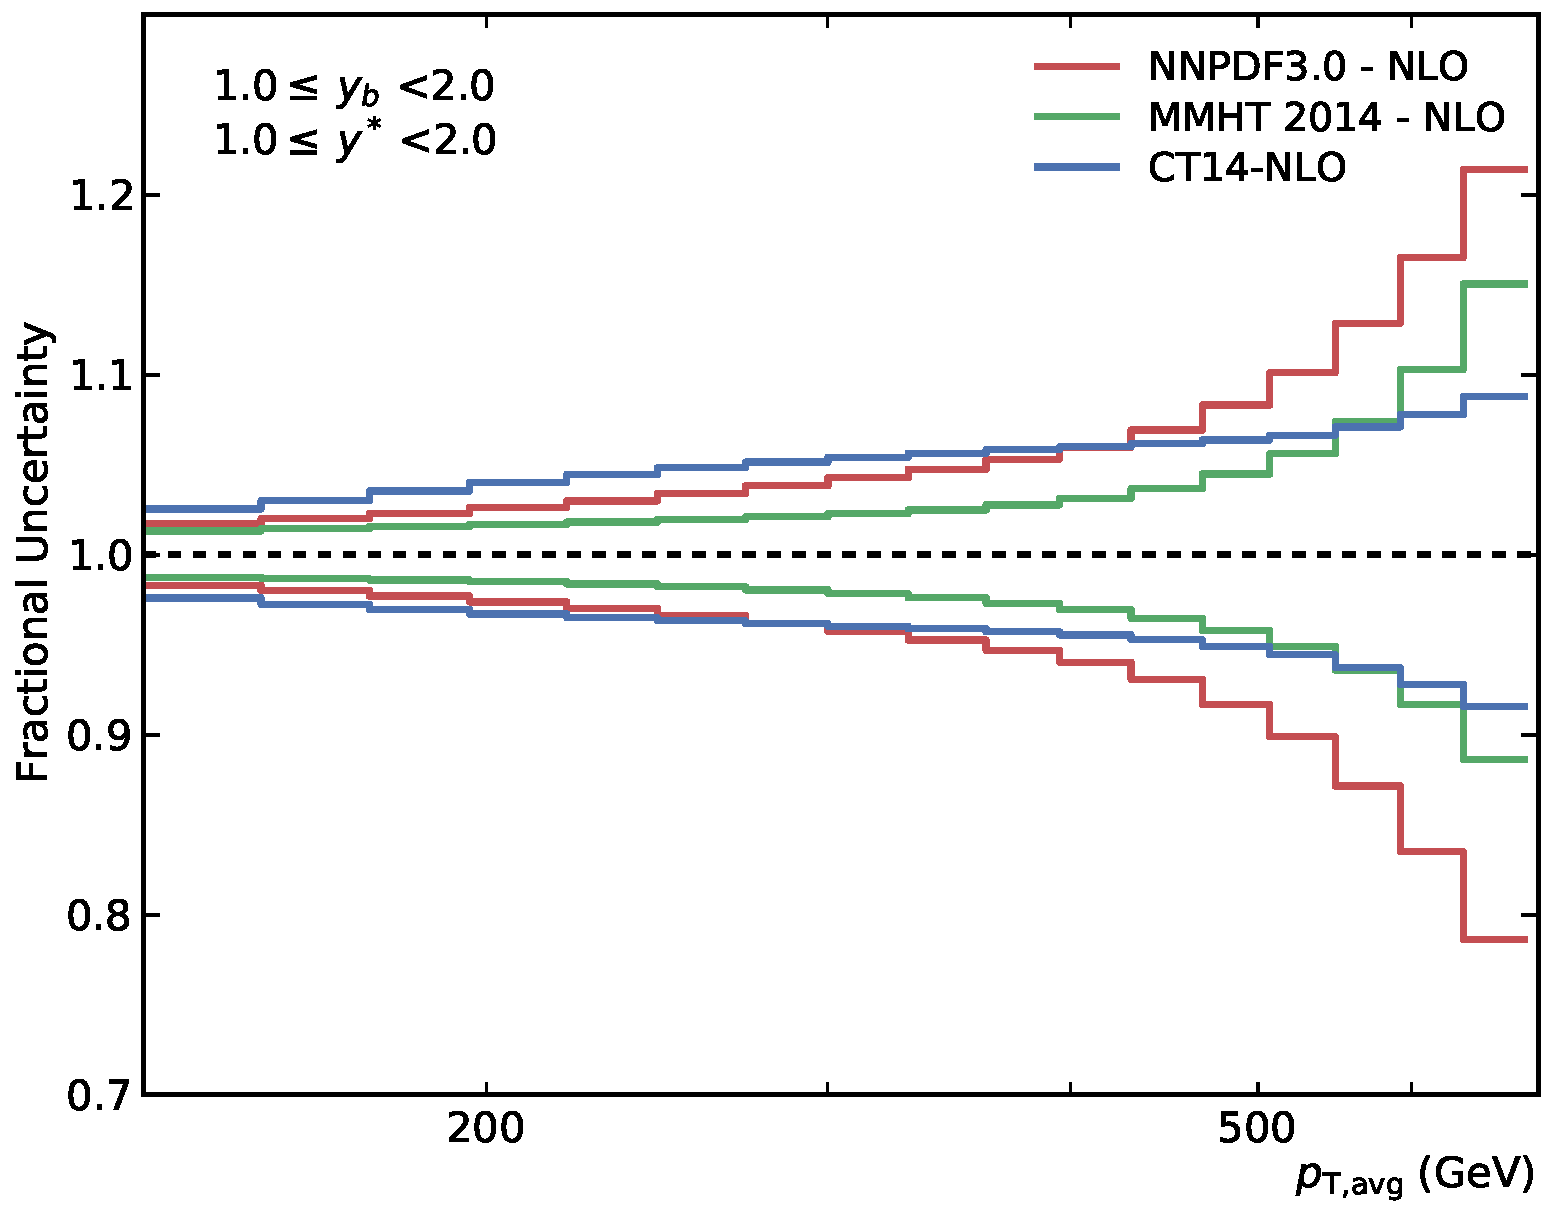
\includegraphics[width=0.45\textwidth]{figures/theory/pdf_unc_comparison_yb1ys1.pdf}\hfill
    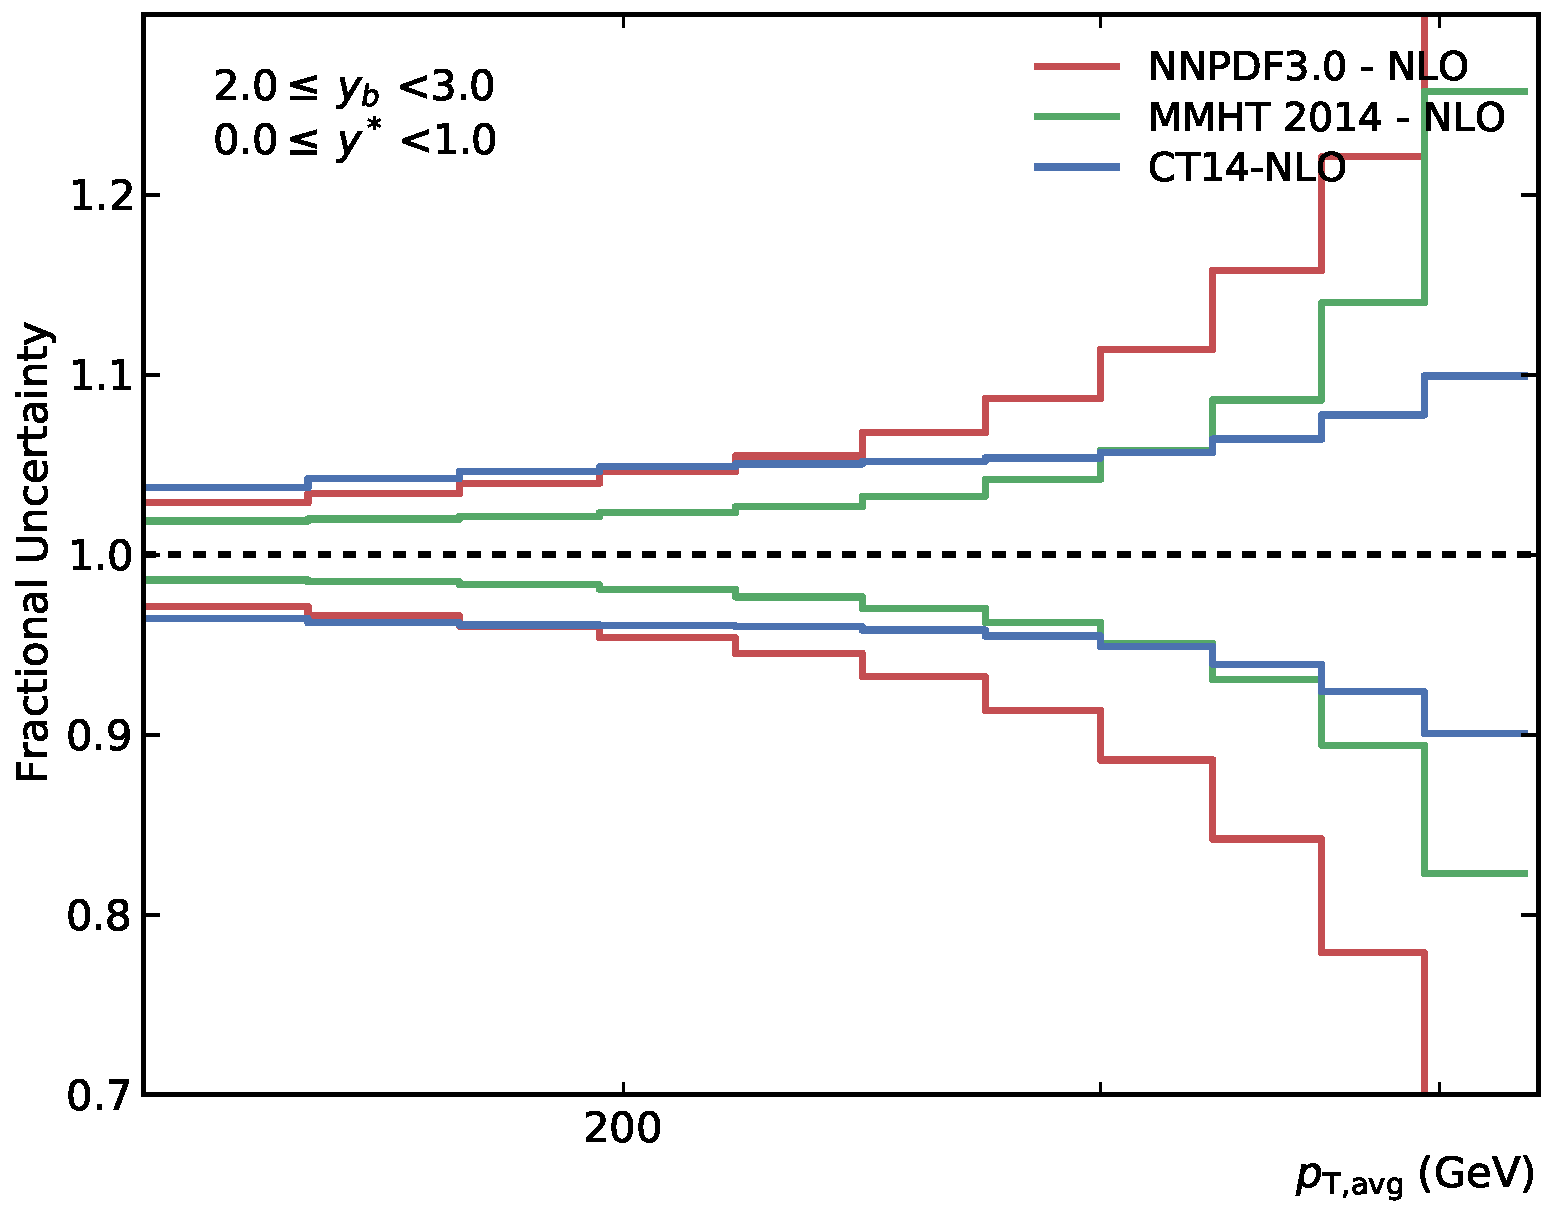
\includegraphics[width=0.45\textwidth]{figures/theory/pdf_unc_comparison_yb2ys0.pdf}
    \caption{The relative PDF uncertainty calculated using the three PDF sets
    NNDFP 3.0, CT14 and MMHT 2014. The uncertainty represents a 68\% confidence
    interval. The PDF uncertainty is sizeable especially in the forward region in
    which both jets have the same sign and high fractional proton momenta are
    accessed. }
    \label{fig:pdf_uncertainties}
\end{figure}

\begin{figure}[htp]
    \centering
    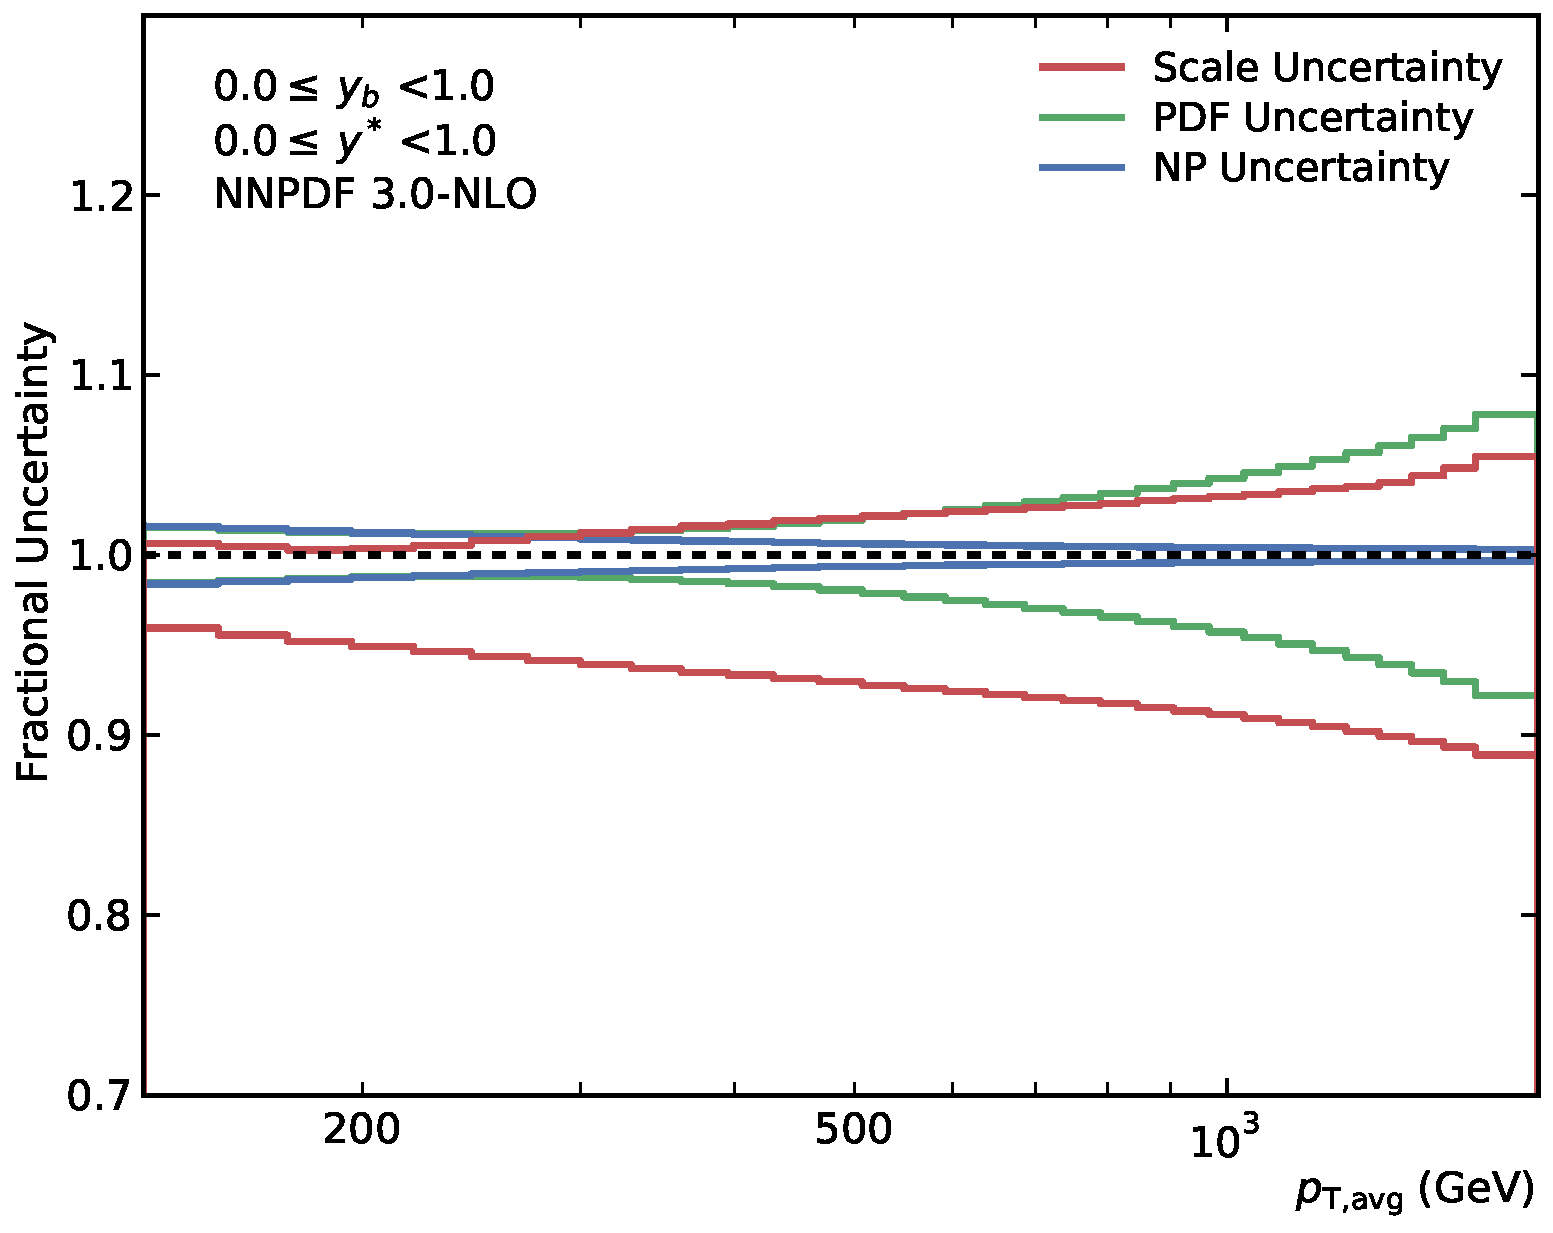
\includegraphics[width=0.45\textwidth]{figures/theory/theo_unc_yb0ys0.pdf}\hfill
    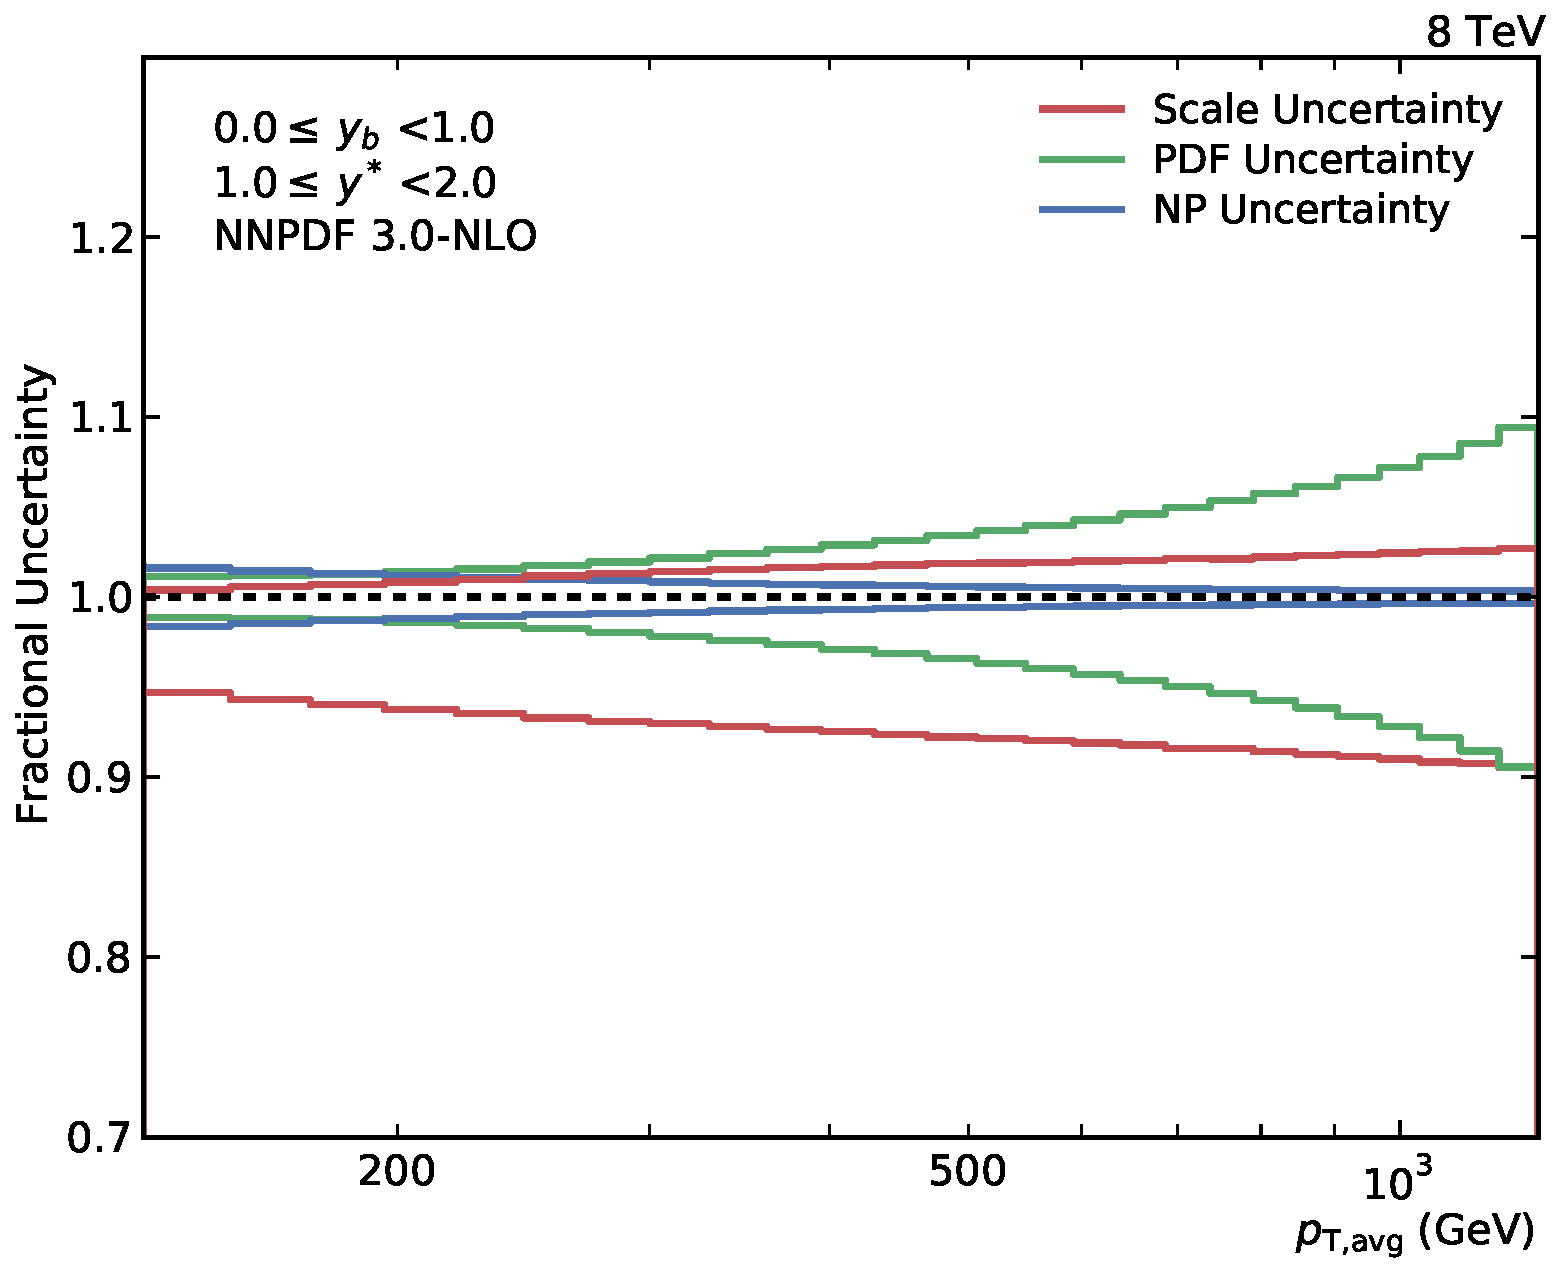
\includegraphics[width=0.45\textwidth]{figures/theory/theo_unc_yb0ys1.pdf}
    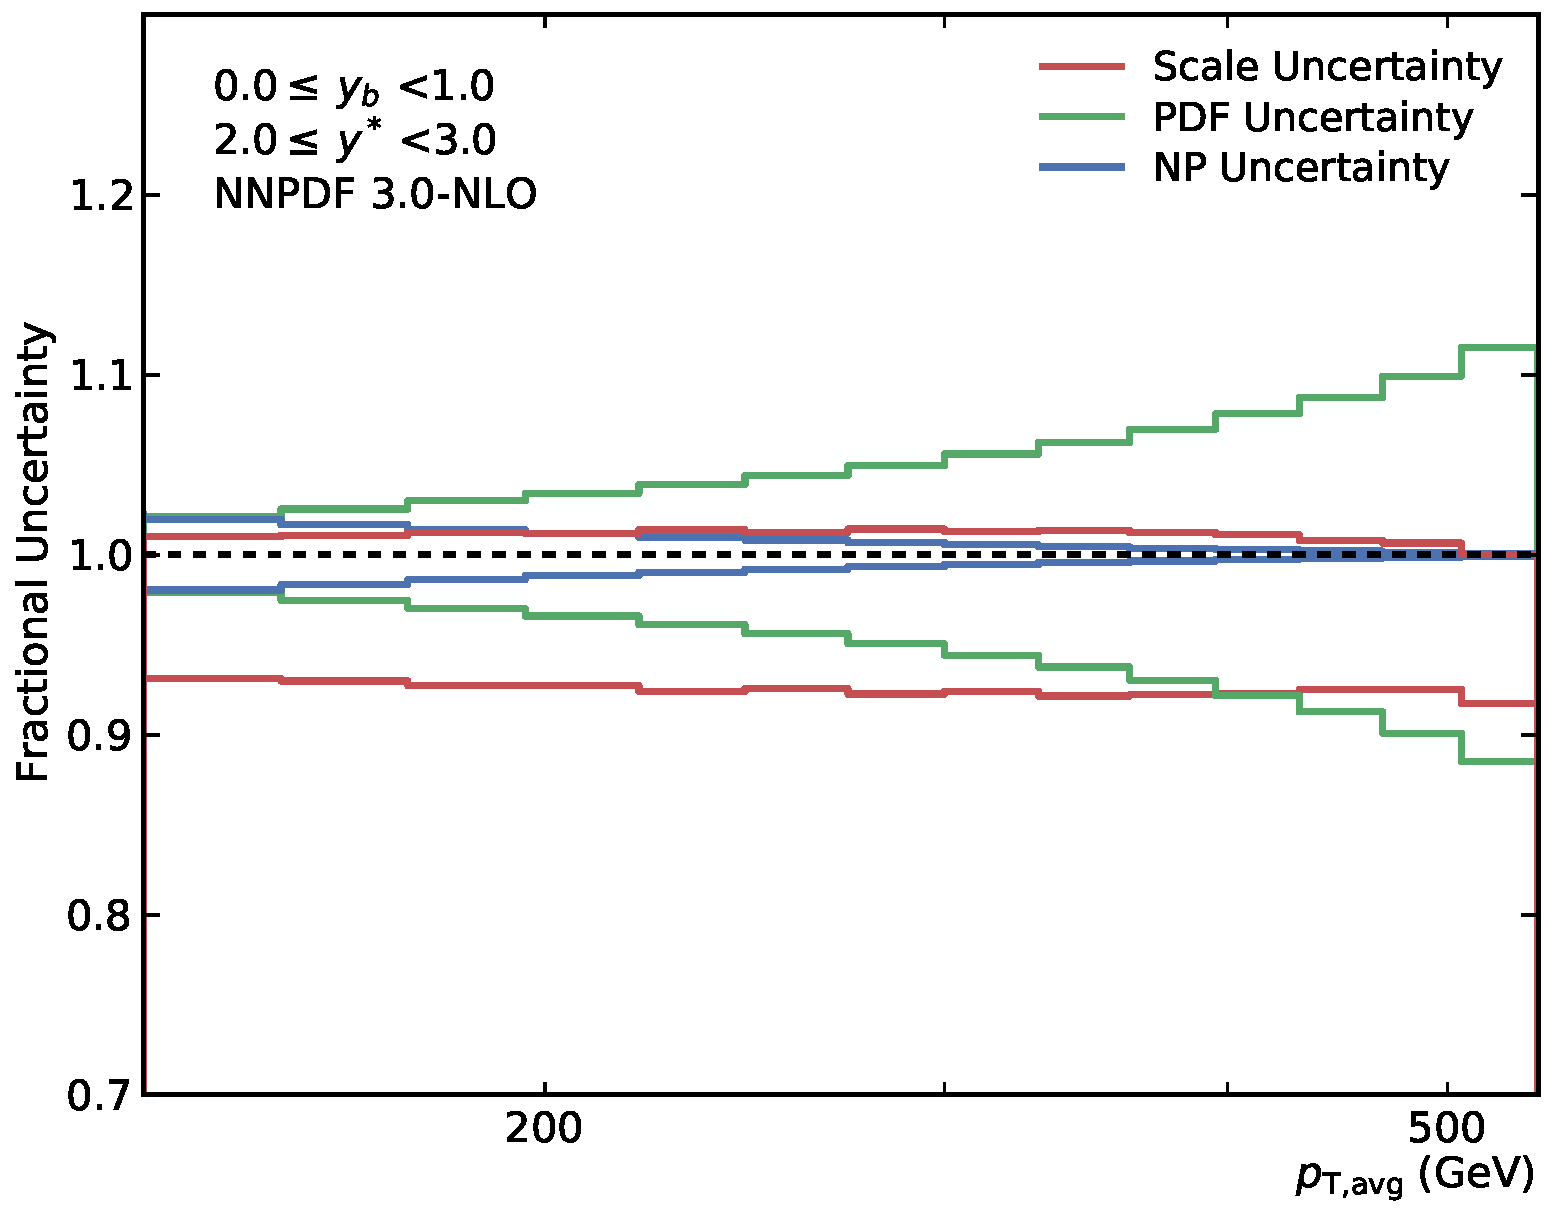
\includegraphics[width=0.45\textwidth]{figures/theory/theo_unc_yb0ys2.pdf}\hfill
    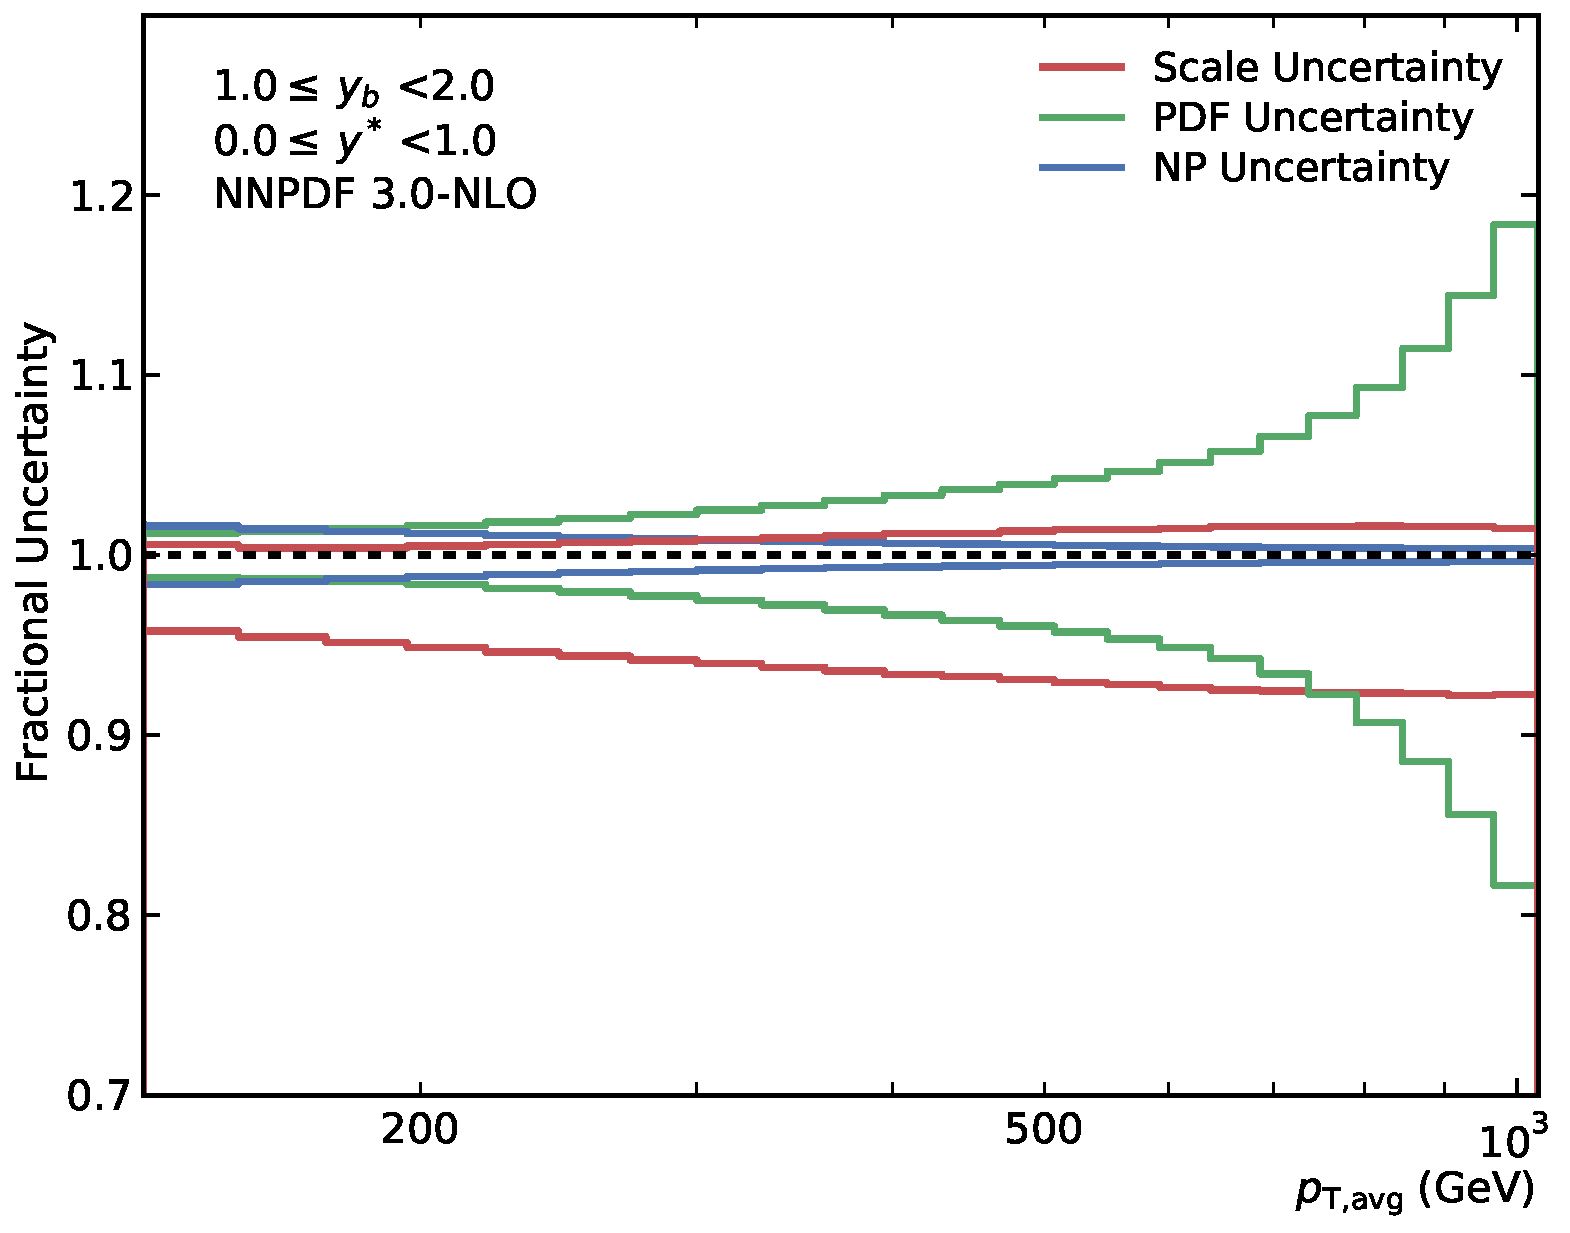
\includegraphics[width=0.45\textwidth]{figures/theory/theo_unc_yb1ys0.pdf}
    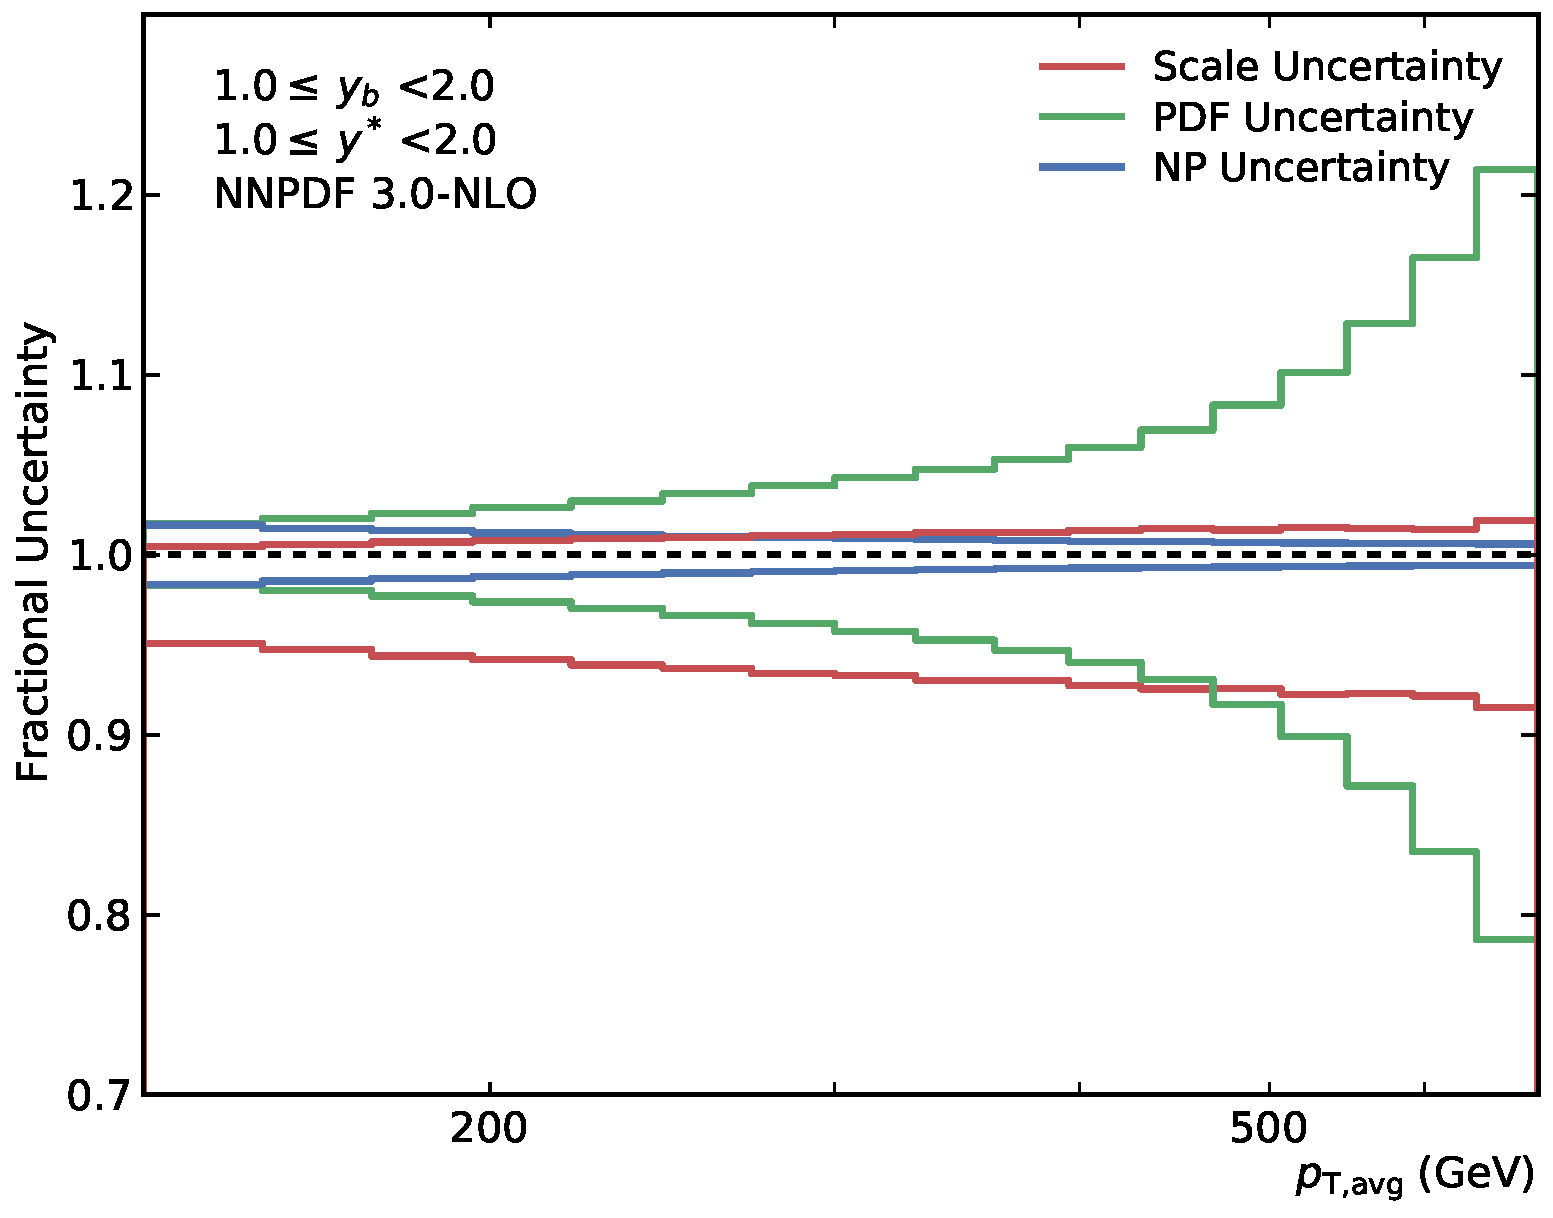
\includegraphics[width=0.45\textwidth]{figures/theory/theo_unc_yb1ys1.pdf}\hfill
    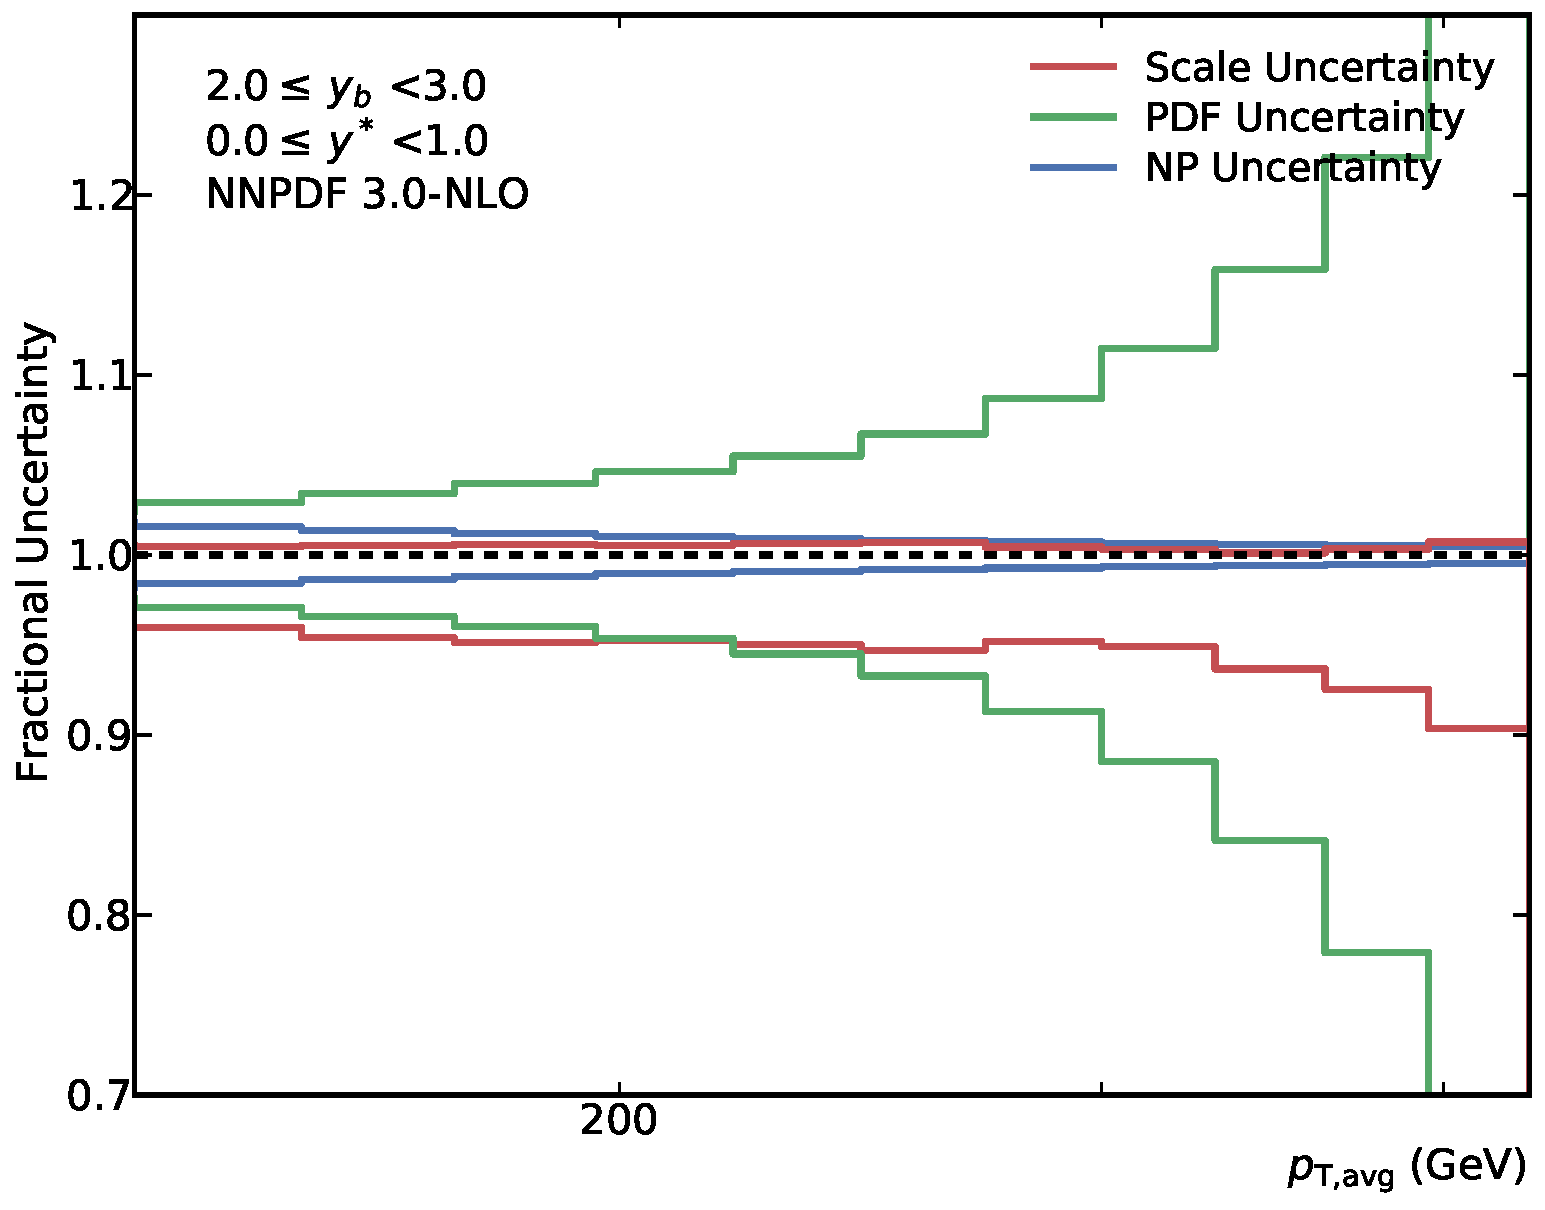
\includegraphics[width=0.45\textwidth]{figures/theory/theo_unc_yb2ys0.pdf}
    \caption{Overview of the theoretical uncertainties of the NLO prediction.
    The scale uncertainty is the dominant uncertainty in the low-\pt region. At
high-\pt and especially in the forward region, the PDF uncertainty becomes
dominant. The NP uncertainty is sizeable only in low-\pt region and becomes
negligible at higher \pt when the NP correction approaches unity.}
    \label{fig:theo_uncertainties}
\end{figure}
